% !TeX root = ../../thesis.tex
\chapter{Real-time genomic epidemiology of SARS-CoV-2 in Belgium}\label{ch:chapter1}

\begin{minipage}[b]{0.57\textwidth}
    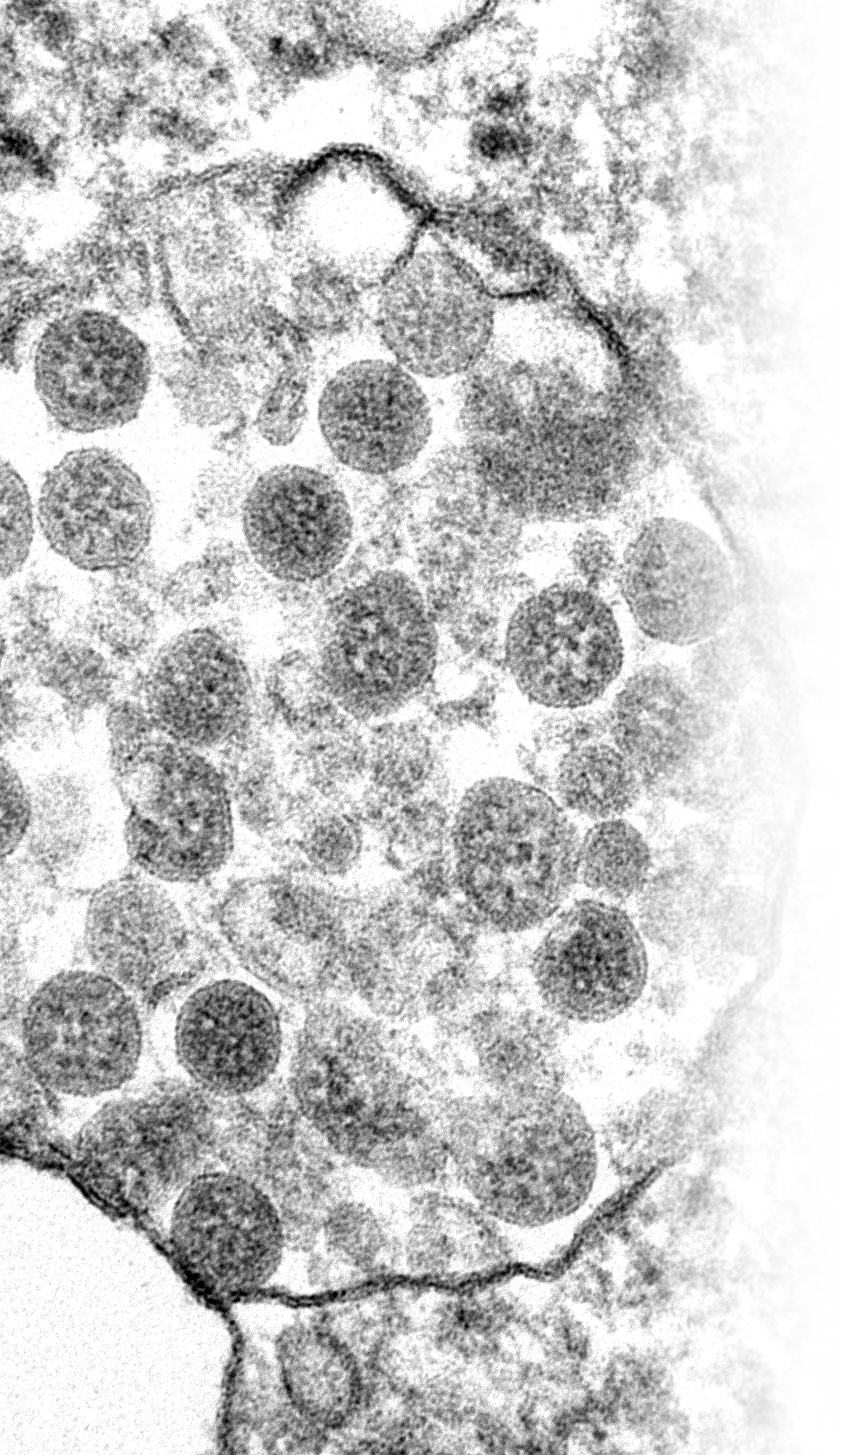
\includegraphics[width=\textwidth]{title2} % Note: image needs to be cropped and faded
    % https://phil.cdc.gov/Details.aspx?pid=23591
  \end{minipage}
  \hfill
  \begin{minipage}[b]{0.35\textwidth}
    \footnotesize
    \begin{flushright}
      \textit{``But in the end it's only\\a passing thing, this shadow;\\even darkness must pass.''} \\
      --- J.R.R.
Tolkien, The Lord of the Rings
    \end{flushright}
    \vspace{2cm}
\end{minipage}
  
\clearpage

\onehalfspacing

\section{Necessities of an ongoing pandemic}
The onset of the COVID-19 pandemic in early 2020 resulted in unprecedented disruption to global public health, economic activity, and daily life worldwide---Belgium was no exception (Fig.~\ref{fig:beCaseCountsRegion}).
The Belgian response to \gls{sarscov2} required rapid development and mobilization of public health infrastructure, including the establishment of nationwide genomic surveillance network.
This surveillance system would ultimately process tens of thousands of viral genomes, generating an unprecedented volume of sequence data that needed to be analyzed and interpreted in near real-time to inform public health decision-making.

% Belgian Case Counts
\begin{figure}[ht]
  \centering
  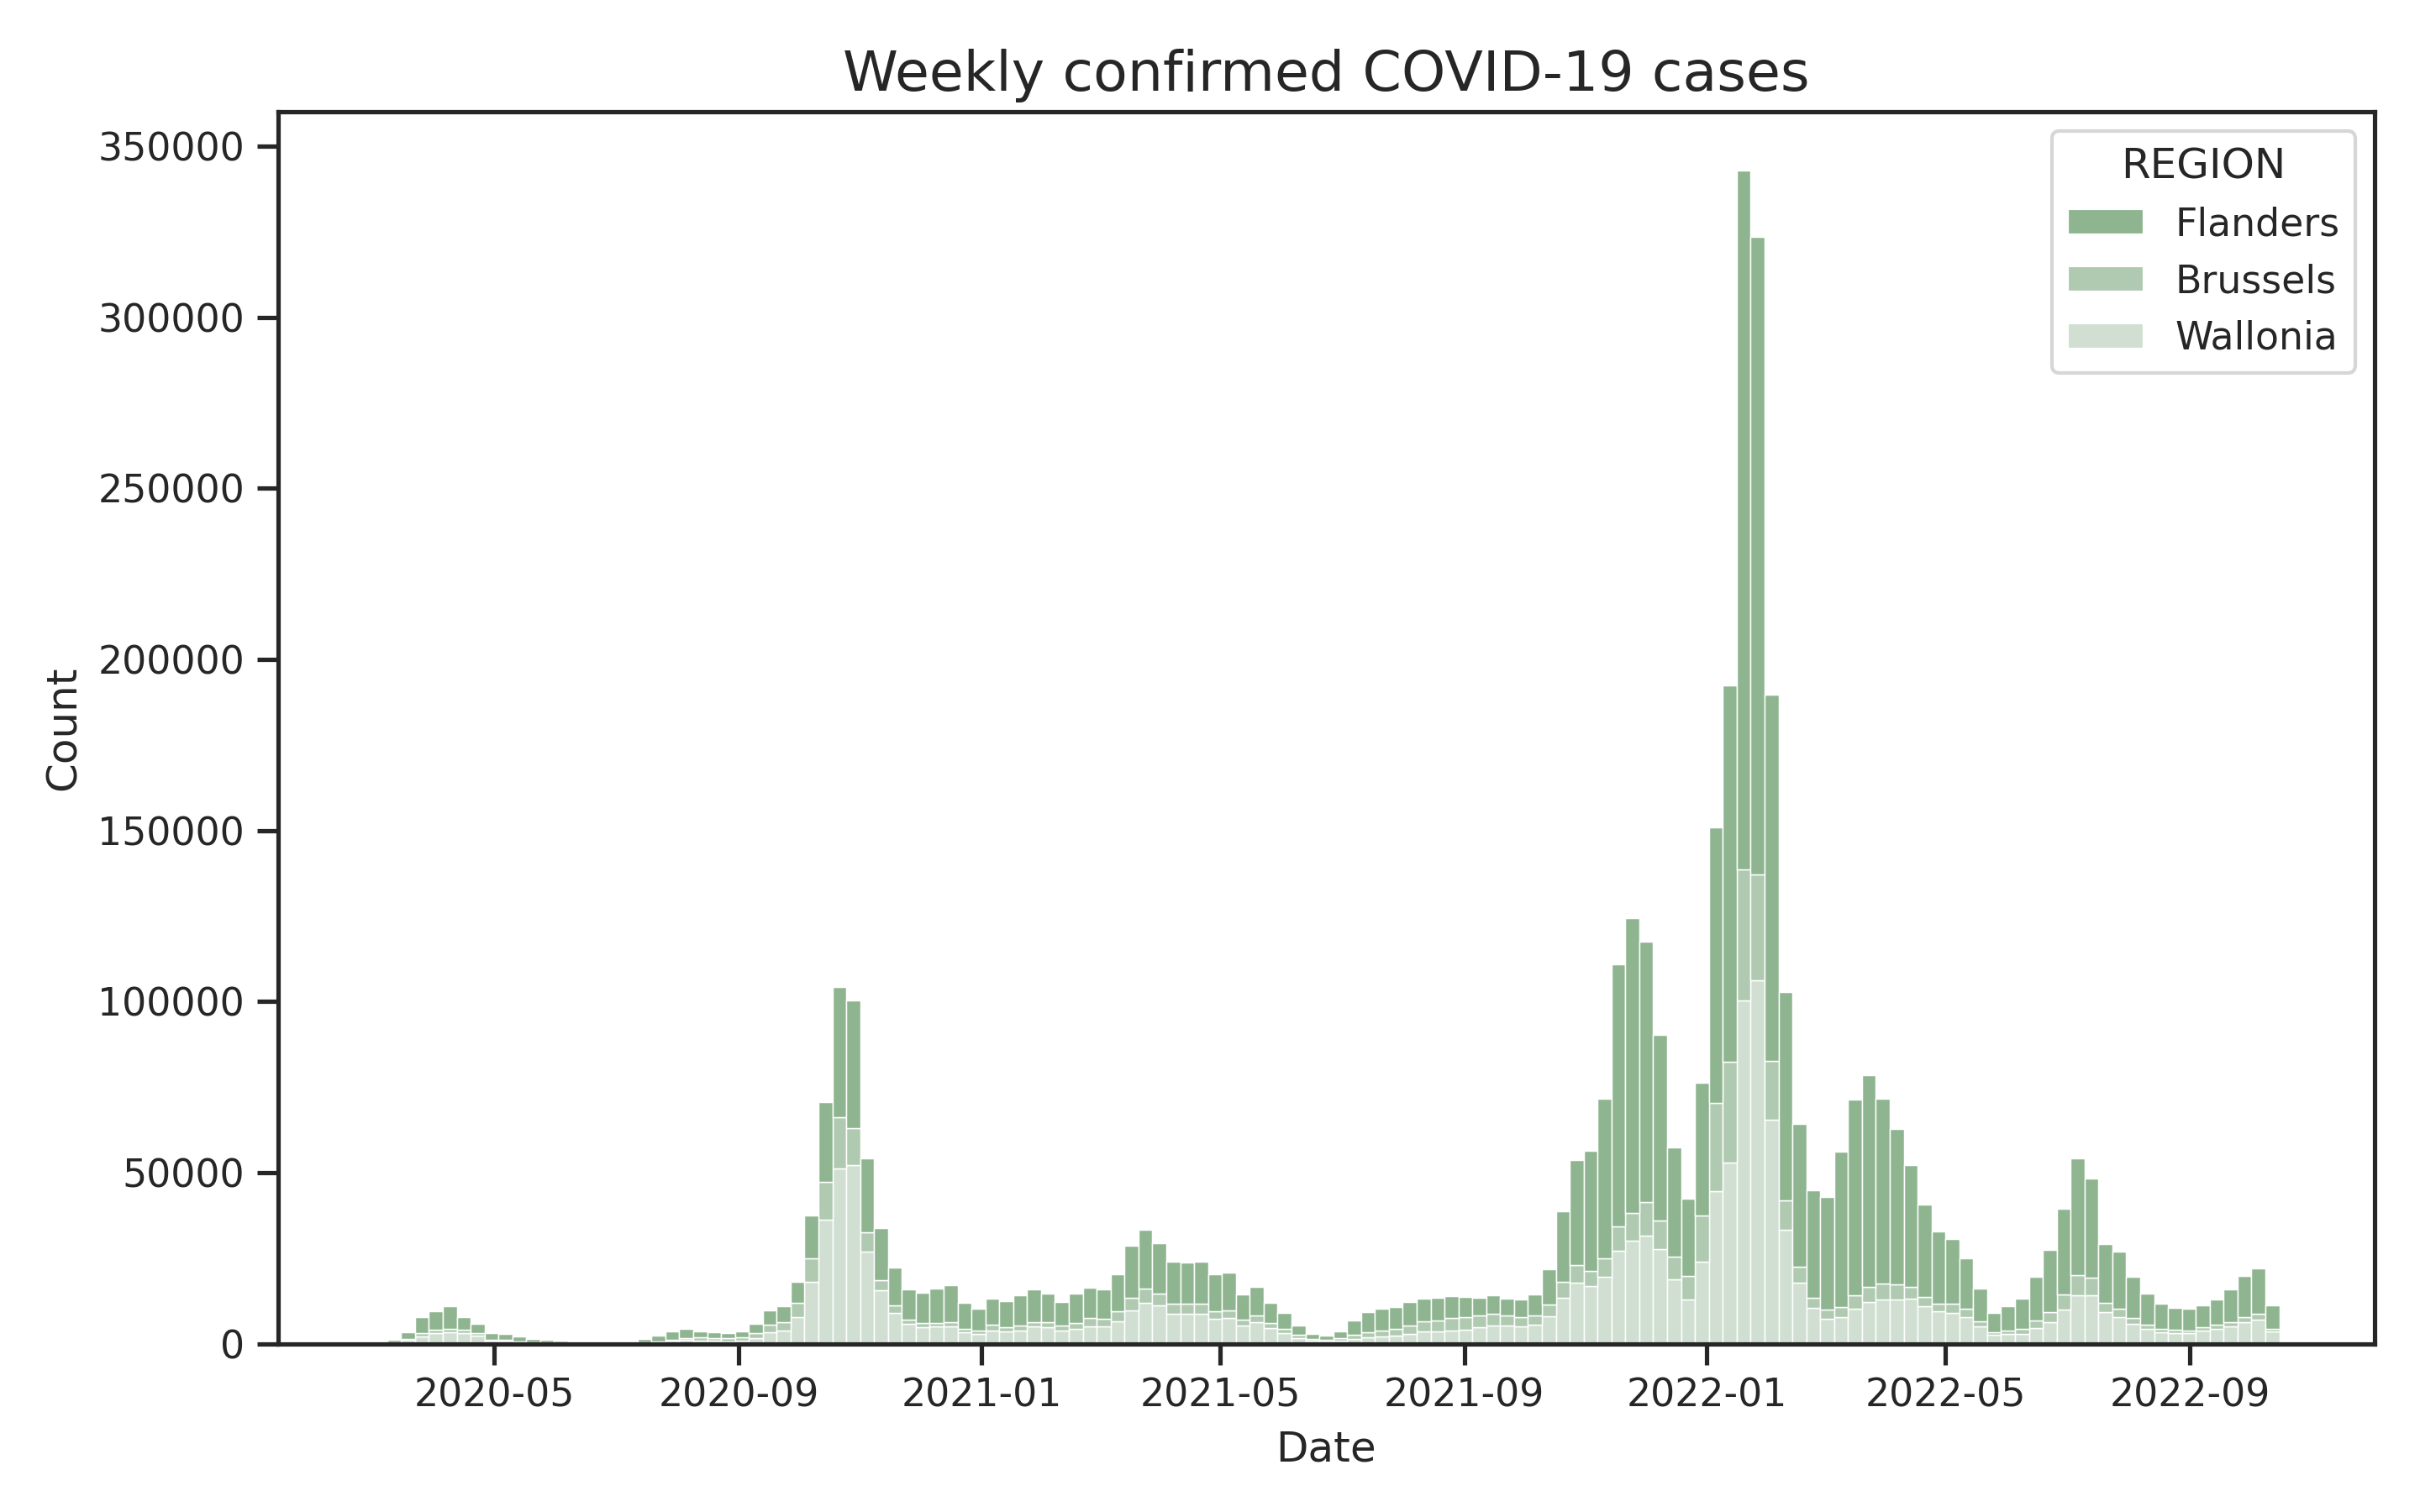
\includegraphics[width=.9\textwidth]{be_cases_region}
  \caption[COVID-19 cases in Belgium by province]{Number of weekly confirmed \gls{sarscov2} cases in Belgium between the beginning of the pandemic and October 2022. Bars are colored by province. \textit{(Data: Sciensano)}}
  \label{fig:beCaseCountsRegion}
\end{figure}

Perhaps the most significant challenge was in maintaining the quality of analyses while operating under intense time pressure.
The rapid evolution of \gls{sarscov2}, emergence of new \gls{voc} lineages (Fig.~\ref{fig:beVoc}), and changing public-health intervention landscape meant that analytical methods needed to be both robust and adaptable.
This required constant refinement of bioinformatic pipelines, regular updates to reference datasets, and ongoing communication with international partners to ensure that Belgian surveillance efforts remained aligned with global standards.
The system needed to be sufficiently flexible to incorporate new types of data and analysis methods as our encoding viral metadata shifted, and needed to be adapted frequently as the number of available genomes rapidly outscaled any previously established analysis methodologies.

\begin{figure}[ht]
  \centering
  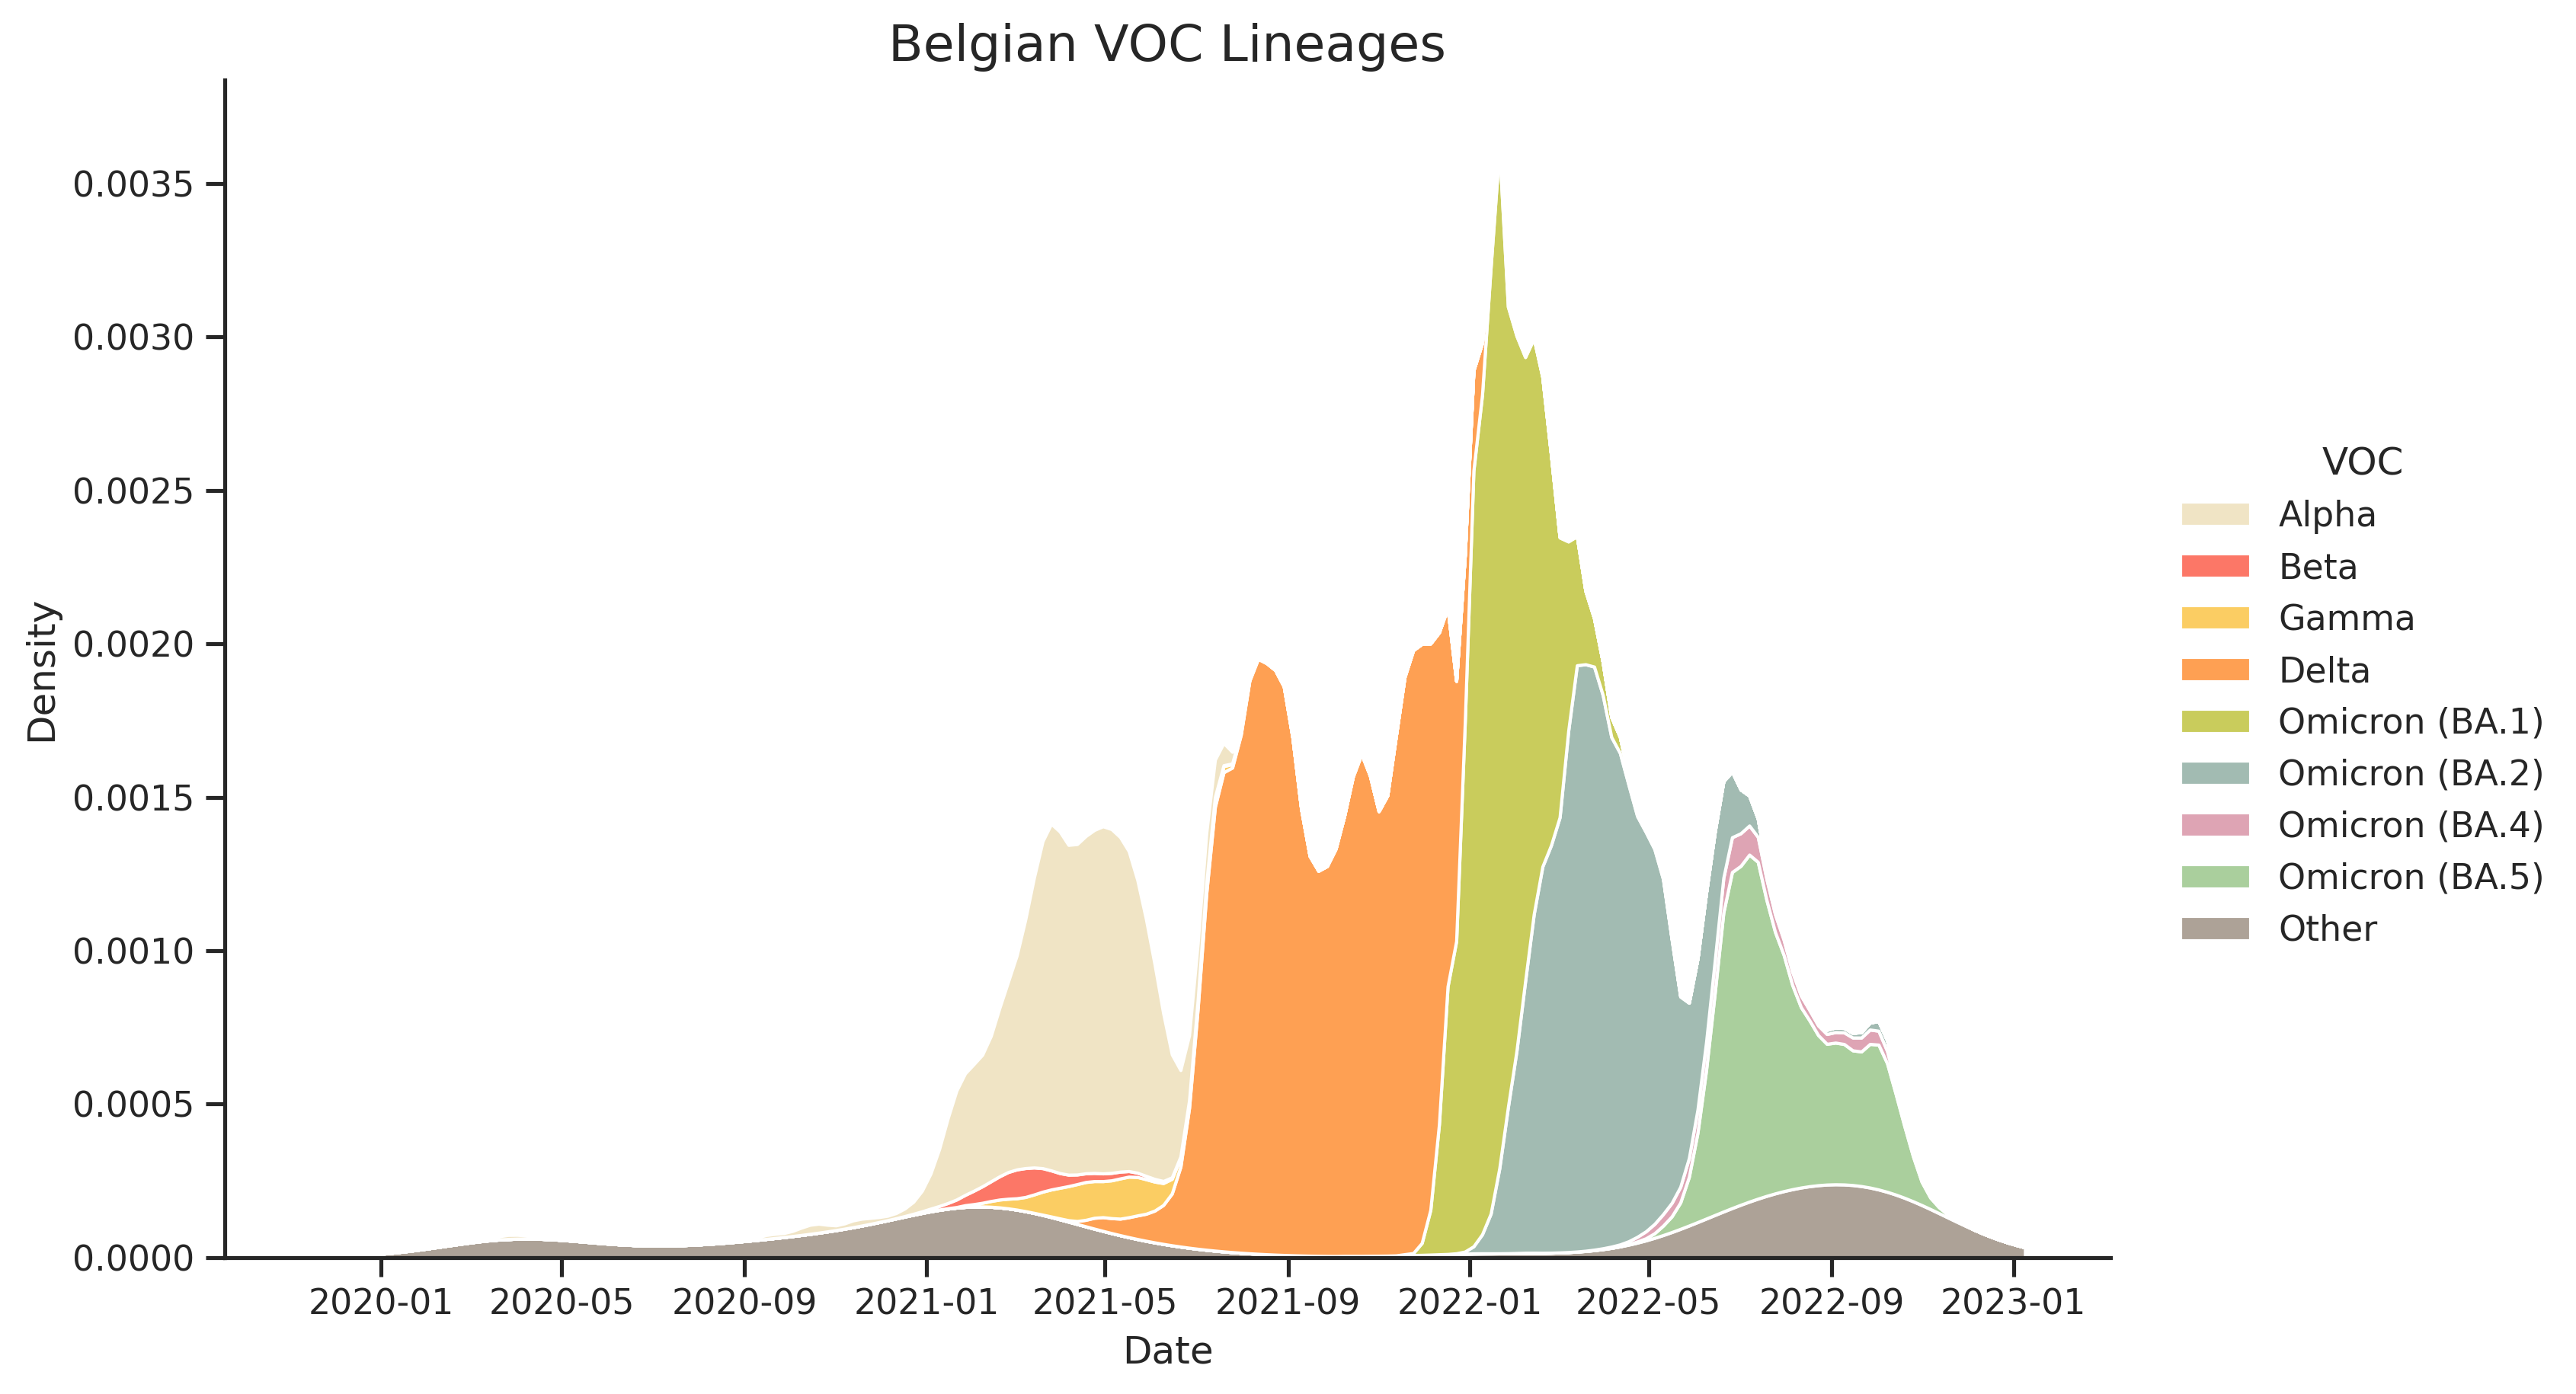
\includegraphics[width=.9\textwidth]{belgium_voc_sequences}
  \caption[VOC sequences in Belgium]{Distribution of genomes on GISAID from Belgium during the pandemic belonging to different \gls{voc} lineages.}
  \label{fig:beVoc}
\end{figure}

We developed a rapid-analysis pipeline that allowed timely phylodynamic analysis of the \gls{sarscov2} epidemic in Belgium.
This pipeline was updated several times weekly as new Belgian genomes became available, and as new lineages of the virus emerged globally.
Our pipeline allowed us to rapidly communicate the most up-to-date situation with all stakeholders: other researchers within Belgium, members of the Belgian Consultative Committee (shown in more detail in Section~\ref{sec:sitRep}), and to the public at large via social media.
Additionally, the dataset construction and maximum likelihood phylogenetic tools included in pipeline were used as a first step in several peer-reviewed research papers both within Belgium (reviewed in Section~\ref{sec:twoYears}) and with international collaborators \citep{dudas2021emergence,holtz2024emergence} as the pandemic progressed.

\section{Real-time genomic epidemiology in Belgium}\label{sec:nextstrainBE}
In order to handle the rapidly-evolving landscape of the \gls{sarscov2} epidemic in Belgium, we chose the adapt the Nextstrain \citep{hadfield2018nextstrain} platform for our specific needs.
Nextstrain represented the most cutting-edge front-to-back maximum likelihood phylodynamics platform available at the time, with tools available for data management, phylogenetic inference, ancestral state reconstruction \citep{huddleston2021augur}, and visualization.
Importantly, Nextstrain was also an open-source platform with a preexisting \gls{sarscov2} analysis pipeline (\url{https://github.com/nextstrain/ncov}) which could be forked and adapted to the Belgium-specific requirements.
Additionally, Nextstrain integrates a web-hosting service that allows anyone who deposits their results on GitHub to share interactive phylogenetic trees and associated metadata with anyone via a URL.
Finally, because it was continually maintained and updated as the pandemic progressed, it was simple to incorporate necessary updates to the Belgian analysis as they became available.
Such updates included lineage definitions, updates to handle rapidly growing datasets, and ``canonical builds'' for a number of different \gls{sarscov2} lineages-by-location combinations wherein the Nextstrain team and their collaborators would release pre-analyzed datasets for many target datasets.

\subsection{Dataset construction}
During the pandemic, the gold-standard repository for \gls{sarscov2} genomic sequence data was the Global Initiative on Sharing All Influenza Data (GISAID) database \citep{shu2017gisaid}, which allowed researchers from around the globe to deposit full-genome sequences and their associated metadata into a single repository.
This database allowed us to filter and download genomes based on a number of relevant features: date, lineage, location, ID, etc.
In 2021, GISAID also added a feature to download all \gls{sarscov2} genomes and their metadata pre-formatted to be processed by Nextstrain's standard toolkit.
All genomes that were analyzed as part of the real-time phylodynamic analysis in Belgium were mediated through GISAID.

Typically, datasets were constructed in a two-step process: assembling a background dataset, and adding target sequences.
Background dataset construction would usually happen once per lineage of interest (\gls{voc} or \gls{voi})---a preexisting canonical Nextstrain build would be identified for a novel lineage of interest, and its sequence identifiers would be downloaded.
We operated under the assumption that canonical builds would contain a representative sampling across space and time of high-quality sequences with which other genomes could be placed.
On occasion, a canonical dataset would be supplemented with sequences the more thoroughly covered a geographic region or span of time---this was particularly important when the specific sources of importations to Belgium were of public-health concern.
Background datasets were fixed for each variant and real-time updates were made only to the target sequences, as described below.

Once background datasets were assembled, specific sets of target sequences were added, depending on the most pressing concerns.
Such updates typically started with the inclusion of all Belgian sequences of the emergent lineage of interest, however Belgium's sequencing capacity quickly outgrew the analytical capacity of our pipeline (Fig.~\ref{fig:gisaidSeq})---and the quantity of sequences was often beyond what was necessary for public-health recommendation---so we developed a process by which we could create a subsampled set of target sequences.
To do so, we would first compile all available sequences that matched the properties (time, lineage, location) that we were interested in analyzing.
Then, sequences would be randomly drawn from different space-by-time bins that were defined in a bespoke manner to achieve the desired number of sequences in each bin.
For a given lineage, $\ell$, we would sample across $i$ different time windows, each with a desired number of sequences ${s_1,s_2,\cdots,s_i}$, defined by our specific goals.
We would select all Belgian sequences from the lineage, $\mathbf{X}_{\ell}$, and partition that set into $i$ mutually exclusive sets, based on their time ($\mathbf{X}_{\ell} = x_1 \oplus x_2 \oplus \cdots \oplus x_i$).
We could then split each of these partitions into $j$ location-based partitions in the same way, leaving us with $i \times j$ total partitions, each with a target number of sequences ($s_{i,j}$).
From each partition, we would sample $s_{i,j}$ sequences uniformly, without replacement, leaving us with a final sample of $\sum_i \sum_j s_{i,j}$ total sequences.

\begin{figure}[ht]
  \centering
  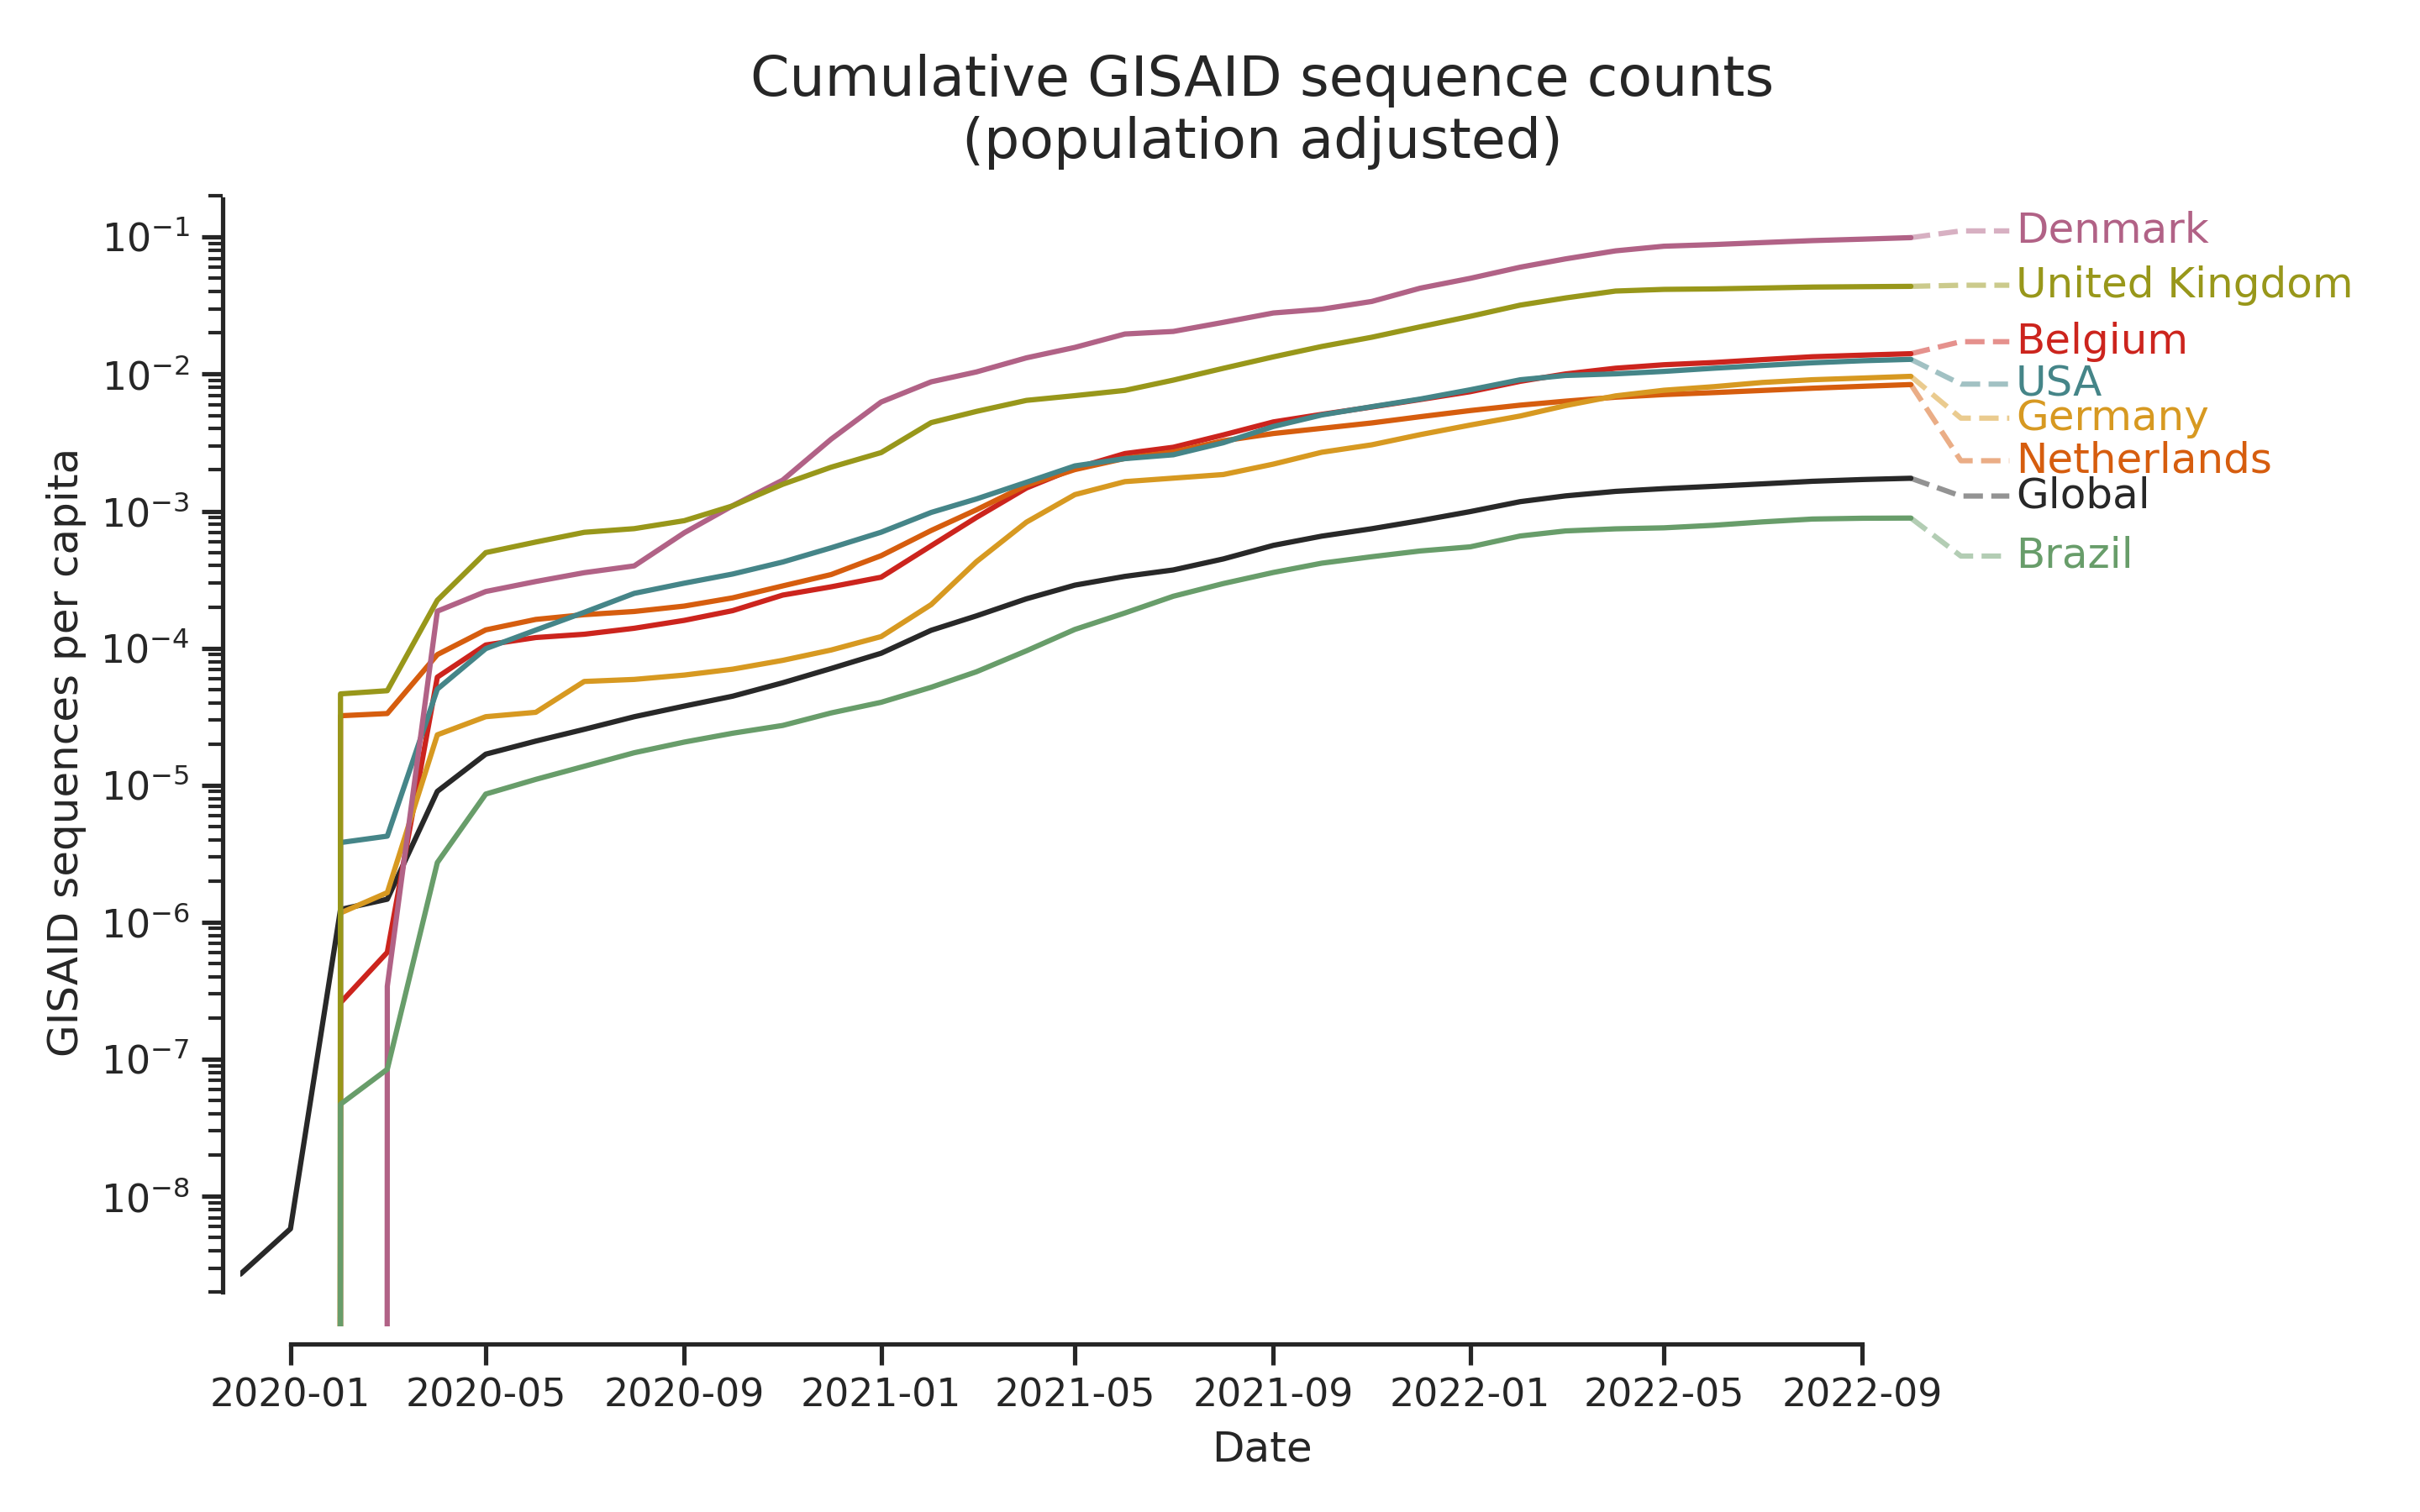
\includegraphics[width=.9\textwidth]{monthly_gisaid_counts_adj}
  \caption[Population-adjusted GISAID sequences]{Cumulative population adjusted count of sequences available on GISAID each month through the first two years of the pandemic.}
  \label{fig:gisaidSeq}
\end{figure}

\subsection{Metadata canonicalization}
It was crucial for each sequence to have accurate geographic metadata to both perform accurate subsampling, as well as to perform ancestral trait reconstruction to quantify the number of importations into Belgium.
To this end, Belgium provided a unique challenge when it came to compiling geographic metadata for sequences on account of its three national languages (Dutch, French, and German).
Early in the pandemic, sequences were not posted to GISAID with any geographic metadata due to concerns with the European General Data Protection Regulation (GDPR), which regulates information privacy.
As a result, we frequently received geographic metadata directly from sequence providers.
These metadata would be encoded in a number of ways (postal code, city name, municipality name), and name-based encoding could be done in any of Belgium's national languages, or English.
For example, sequences coming from Belgium's capital could be labeled as any of \textit{Brussel}, \textit{Bruxelles}, \textit{Br\"{u}ssel}, or \textit{Brussels}, depending on the preferred language of whoever recorded the locations.
Furthermore, such locations were subject to routine spelling errors and different file encodings for the data.
To handle this problem, we developed a pre-processing pipeline that integrated string matching, translations of municipality names, geocoding (for postal codes), and multiple file parsers.
This pre-processing would be run on all metadata that we received in order to both canonicalize the data for analysis, and to ensure that all sequences had a properly encoded hierarchy of locations (municipality, province, region, and country).
This pipeline needed to be updated nearly constantly as new sequences were continually generated until mid-2021, when standards for location-based metadata were standardized for submitters to GISAID.

\subsection{Custom fork of Nextstrain}
In addition to the pre-processing pipeline for metadata, we made several modifications to the original fork of the Nextstrain \verb|ncov| pipeline (Fig.~\ref{fig:beNxt}).
These modifications allowed us to overwrite the default multiple sequence alignment tools, which for many months represented the single biggest computational hurdle that slowed down analyses.
One of the major modifications that streamlined analysis took place when the multiple-sequence alignment tool \verb|nextalign| \citep{aksamentov2021nextclade} was released in 2021.
By adding this alignment tool---which was purpose-designed during the pandemic---instead of the previously used MAFFT \citep{katoh2013mafft}---and a simultaneous change to multiple sequence \textit{after} subsampling we were able to reduce total analysis time to less than a day, typically allowing us to have a total processing time of roughly two days between the time new sequences were deposited in GISAID, and the time that a new build was available to the public (for example Fig.~\ref{fig:firstBeBuild}).

\begin{figure}[ht]
  \centering
  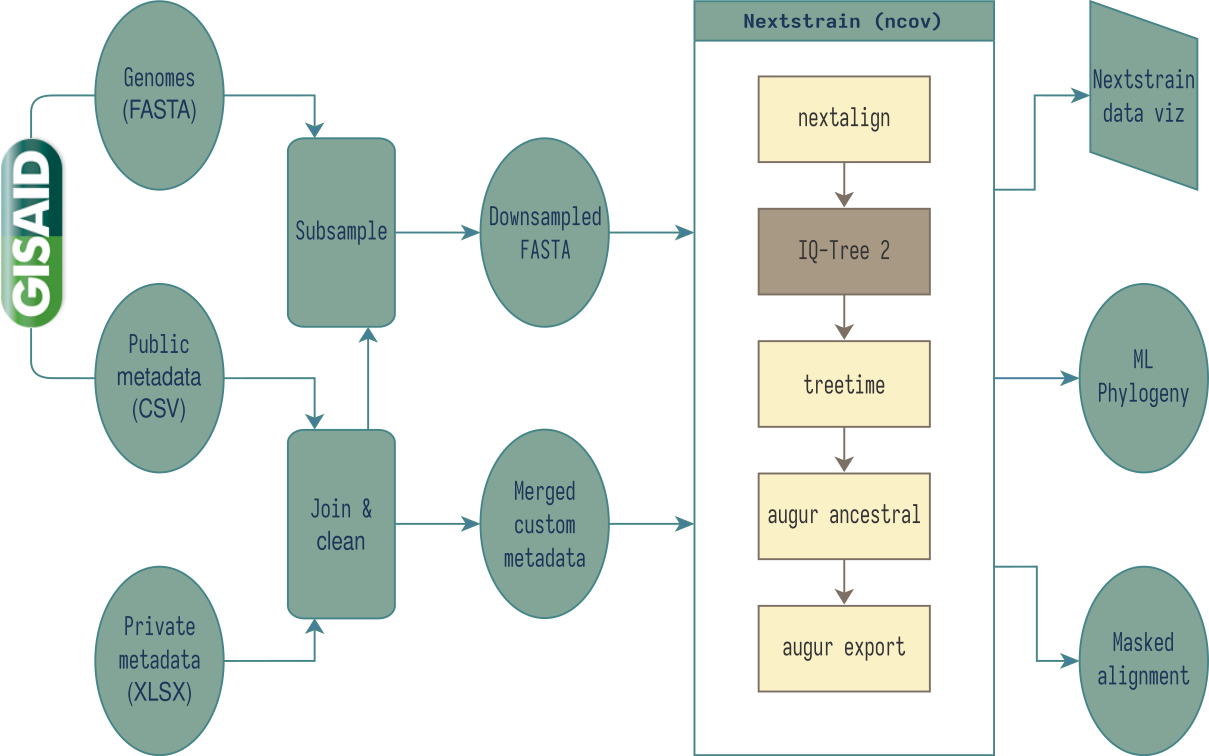
\includegraphics[width=.75\textwidth]{nextstrain_process}
  \caption[Modified Nextstrain pipeline]{Schematic of our modified fork of the Nextstrain pipeline used for real-time genomic epidemiology in Belgium. Steps included in the default Nextstrain \verb|ncov| pipeline (including the tree-building step that we overwrote) are boxed.}
  \label{fig:beNxt}
\end{figure}

In addition to multiple sequence alignment modifications, we would frequently change the parameters of maximum likelihood tree-building, choosing to replace the default \verb|augur tree| option provided by Nextstrain with a custom call to IQ-Tree2 \citep{minh2020iq}, a ML phylogenetic inference program with a version developed for viral sequence data during the pandemic.
While most analyses included fixed arguments to this tree-building step, on occasion we would modify the parameters (typically the type of nucleotide substitution model) in response to analysis-specific requirements.
The entirety of the modified fork, as well a version history containing all historical builds, are available at \url{https://github.com/GuyBaele/sars-cov-2-belgium}.
The most-recent versions of public builds can be accessed at \url{https://nextstrain.org/community/GuyBaele/sars-cov-2-belgium?c=clade_membership&f_country=Belgium}, however due to the extremely rapid turnover of builds many of the builds were treated as ephemeral and can only be found in the version history of the repository.

\begin{figure}[ht]
  \centering
  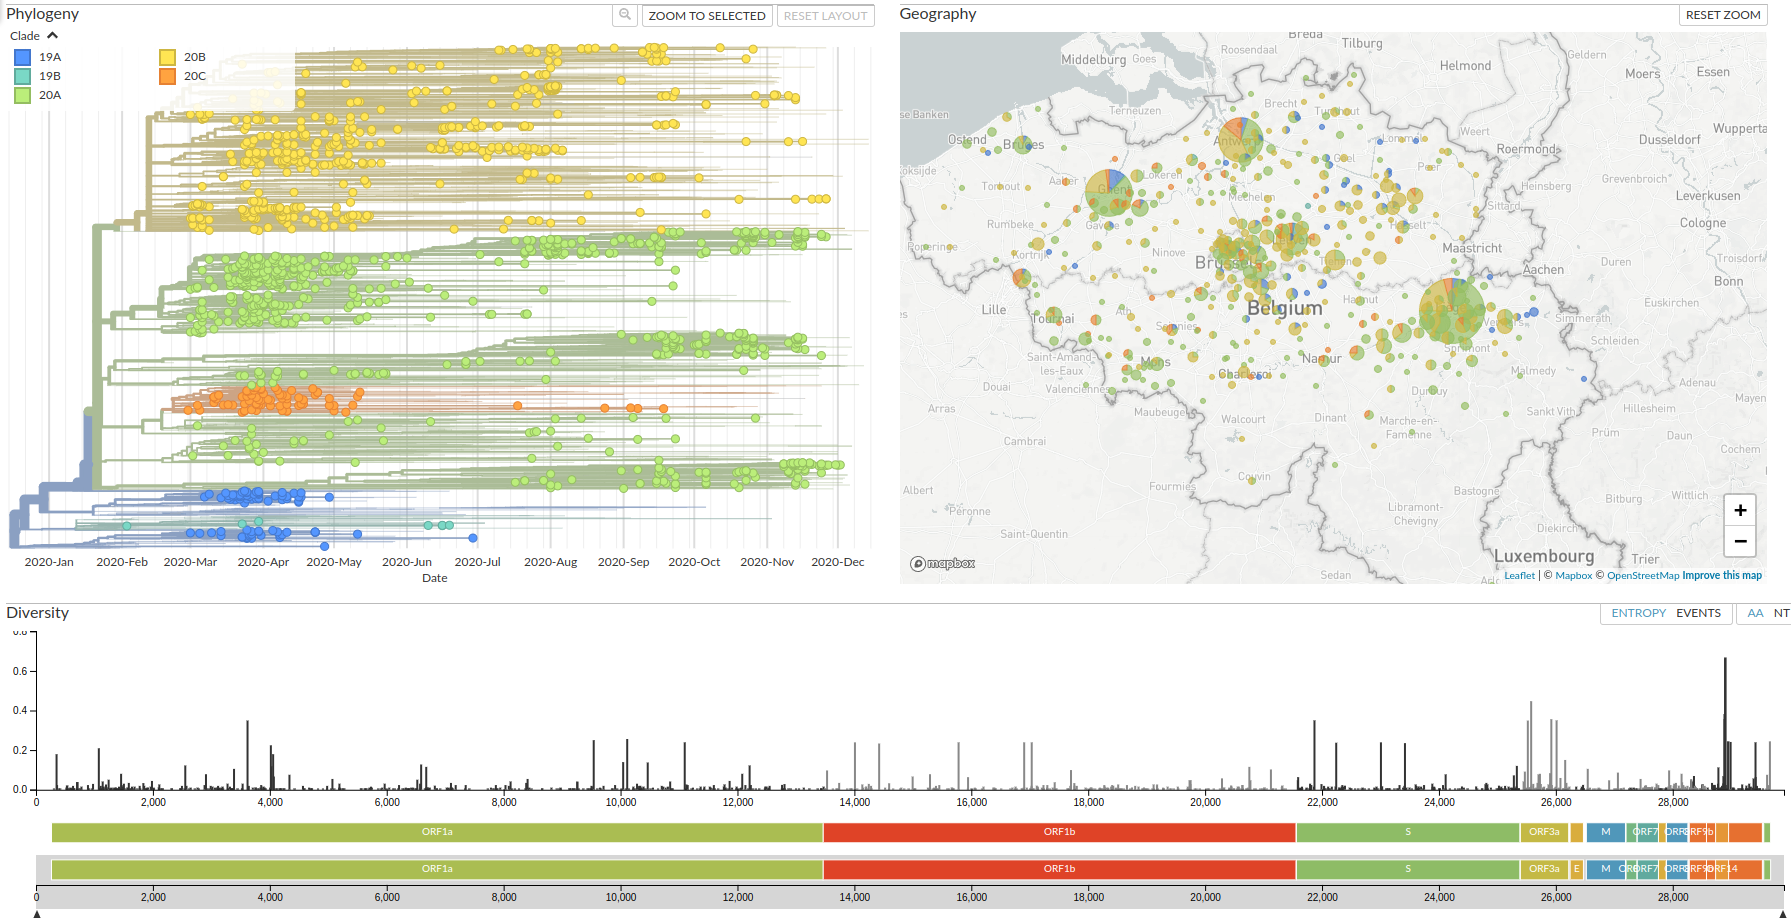
\includegraphics[width=.95\textwidth]{initial_belgian_build}
  \caption[First Belgian Nextstrain instance]{Screenshot of the first public Nextstrain Belgium build. Each build displays three key windows: \textit{(top left)} an interactive phylogenetic tree which can be colored by a number of traits (e.g. clade, location, mutation), \textit{(top right)} a map of Belgium with pie charts representing total number and distribution of the colored trait on the phylogeny, and \textit{(bottom)} a schematic of the \gls{sarscov2} genome representing the relative diversity of each position in the genome.}
  \label{fig:firstBeBuild}
\end{figure}

\section{Situation reports}\label{sec:sitRep}
\singlespacing
\hrule
\vspace*{12pt}
The following section includes excerpts from three of the 102 Belgian genomic surveillance reports written between 17 January 2021 and 8 November 2022.
The more than one situation report per week were coauthored by many members of the COVID-19 Genomics Belgium consortium, and came in the form of rapid communiqu\'{e}s intended for the Belgian Consultative Committee---the panel of experts who directly advised policymakers on the status of the pandemic and appropriate intervention strategies.

I have chosen to include excerpts from three such reports, each of which represents a core feature of the reports.
In all cases, I have chosen to include the excerpts and figures that best represent my own personal contribution to the authorship of these reports---typically in the form of Nextstrain trees or phylogenetic insights---and included the results of others only where they are appropriate to contextualize my own work.

The first report we ever released is included, as it coincided with the emergence of the three \gls{voc} lineages that would go on to be known as Alpha, Beta, and Gamma.
The second report presented in this thesis came from a time when all three of the original \gls{voc}s were circulating, representing one of the periods where we reported ``baseline'' genomic surveillance to the Consultative Committee.
Finally, a report highlighting an emergent \gls{voc} (Delta) in the middle of its rise to fixation from the summer of 2021 is presented.
These three reports represent a small sampling of how real-time phylodynamic inferences were generated and reported to public health officials in Belgium during the first year of the pandemic.
\vspace*{12pt}
\hrule
\onehalfspacing

\subsection{First genomic surveillance report: 17 January 2021}
\subsubsection{Executive summary}
Genomic surveillance has scaled-up as decided on \nth{29} of December 2020, with over 1.100 recent viral genomes sequenced. Approximately 1/3 of these genomes could be analysed, highlighting that Belgium has recently experienced multiple introductions of variants of concern (\gls{voc}s). The consolidated epidemiological data are consistent with documented events of local transmission, including at least one large community outbreak.
The trend in ``S dropouts'' among \gls{pcr} results obtained in the Federal Platform laboratories are consistent with a recent phenomenon steadily increasing over the recent days.

\subsubsection{International context}
Since the end of the year, 3 variants of concern (\gls{voc}s) have arisen independently of one another in the United Kingdom (501Y.V1), South Africa (501Y.V2) and Brazil (501Y.V3).
These variants harbour a number of mutations and deletions associated with higher infectiousness and immune escape.
All 3 variants are spreading internationally, with 501Y.V1 and 501Y.V2 having been detected in Belgium.

\begin{figure}[ht]
  \centering
  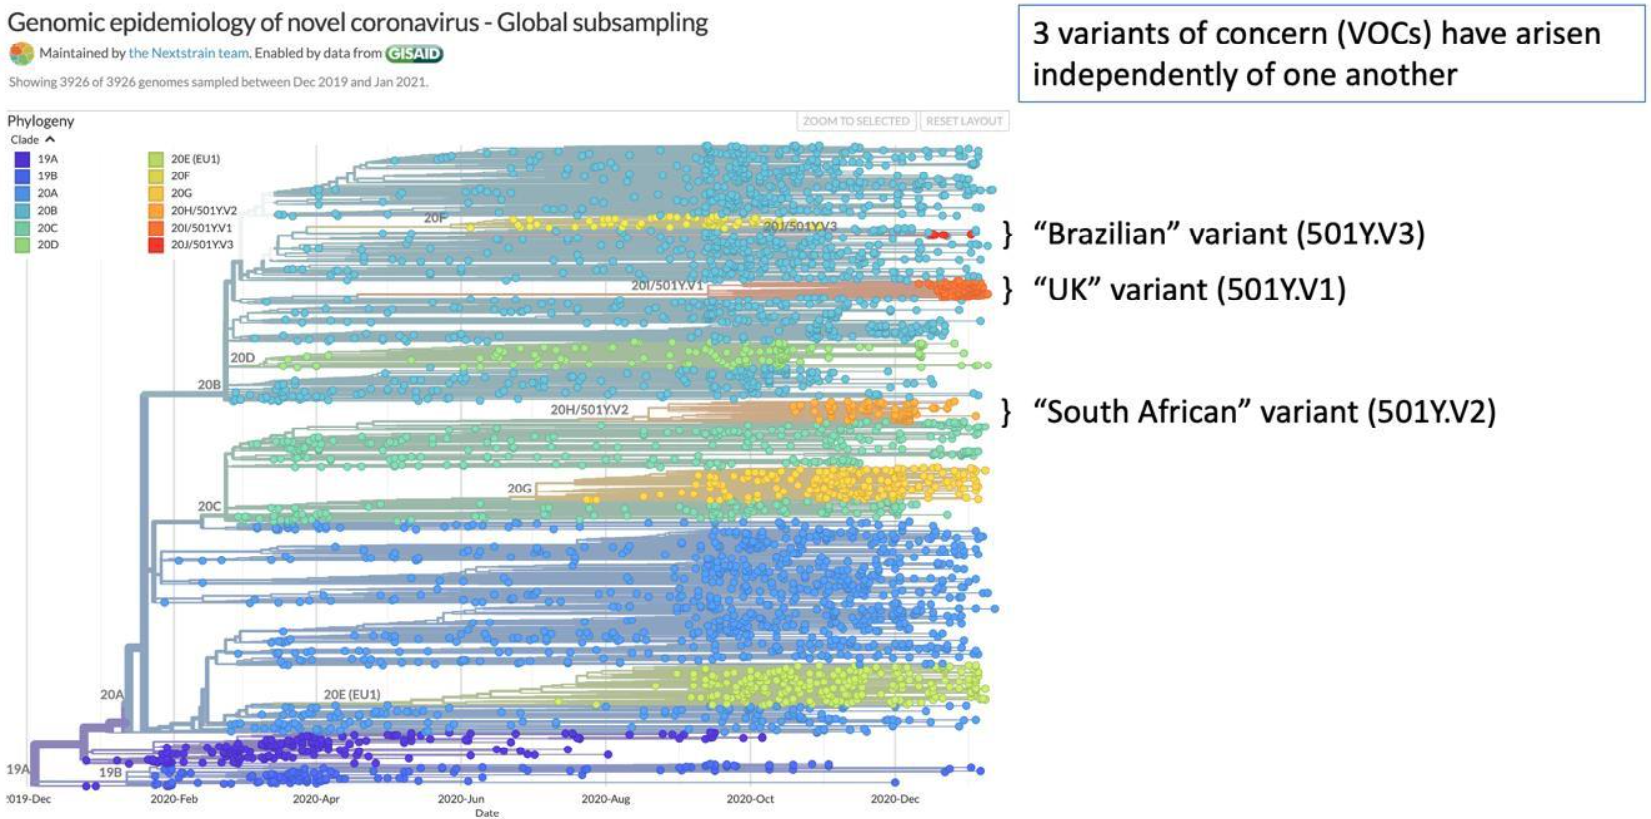
\includegraphics[width=.8\textwidth]{sitRepFirstVOC}
  \caption[Global view on the 3 variants: 501Y.V1, 501Y.V2 and 501Y.V3]{Global view on the 3 variants: 501Y.V1, 501Y.V2 and 501Y.V3.}
  \label{fig:sitRepFirstVOC}
\end{figure}

\begin{figure}[ht]
  \centering
  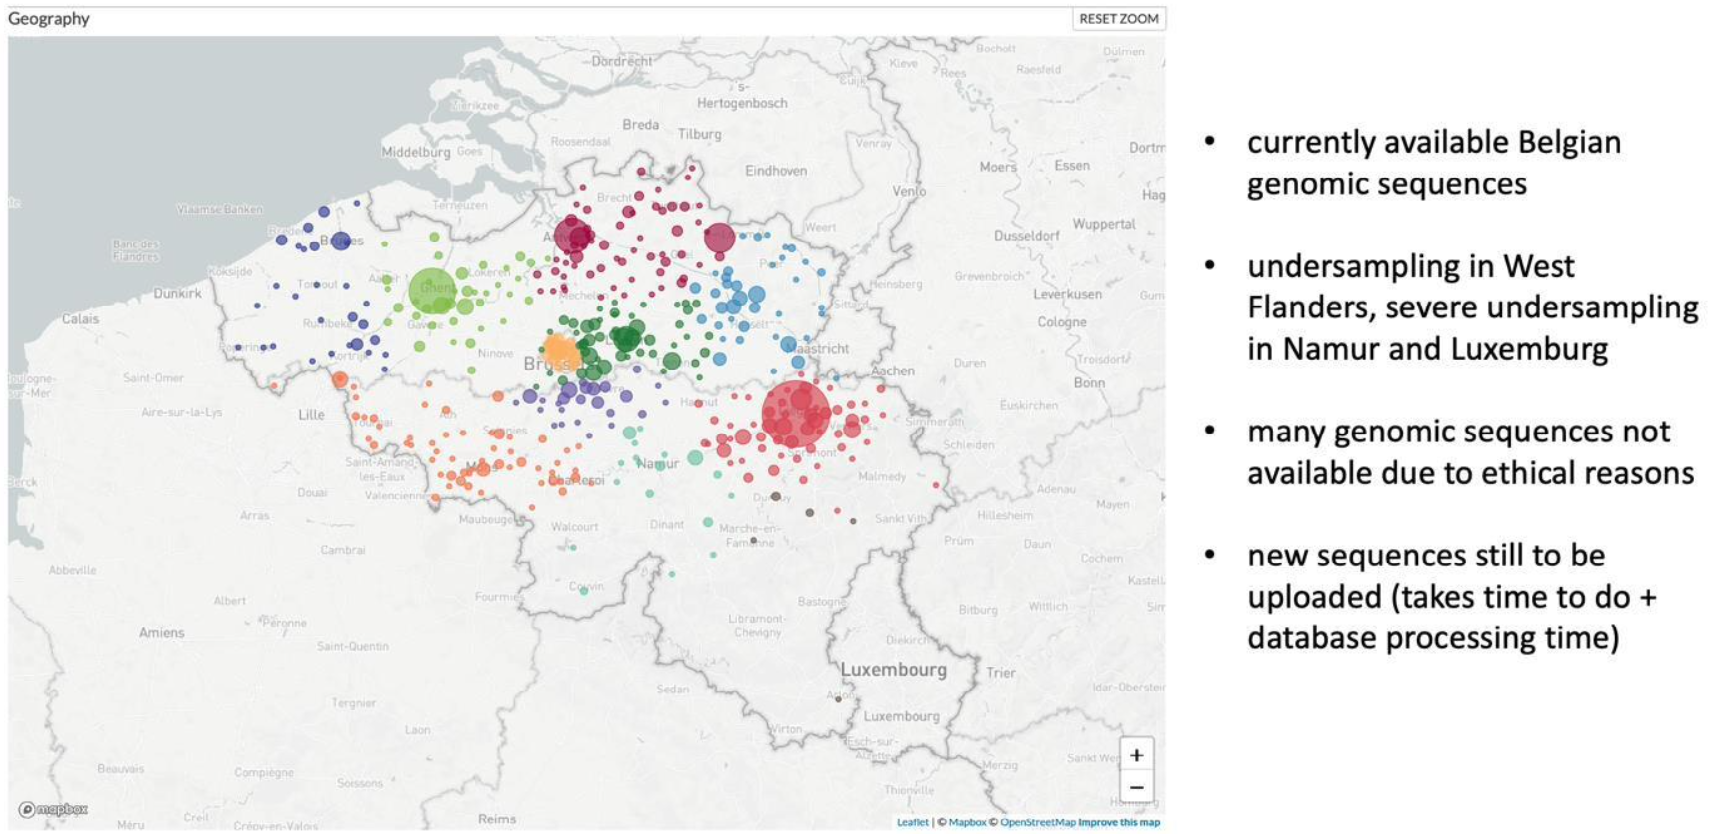
\includegraphics[width=.8\textwidth]{sitRepCoverage}
  \caption[Coverage by province of available sequences]{Coverage by province of available sequences.}
  \label{fig:sitRepCoverage}
\end{figure}

\subsubsection{Recent introduction of \gls{voc}s in Belgium}
Of the 91 501Y.V1 and 7 501Y.V2 identified by the sequencing platforms, only 7 501Y.V1 sequences were available on GISAID on the 16th of January.
The phylogenetic analysis of these sequences show that these originated from 4 individual introduction events, with a first case of local transmission in Belgium.
Although most of the \gls{voc} genomes are not yet included in the analysis hereunder, we know from the context of the latest \gls{voc}s detected that both 501Y.V1 and 501Y.V2 have generated secondary infections in Belgium and that 501Y.V1 has been involved in at least one large community outbreak.

\begin{figure}[ht]
  \centering
  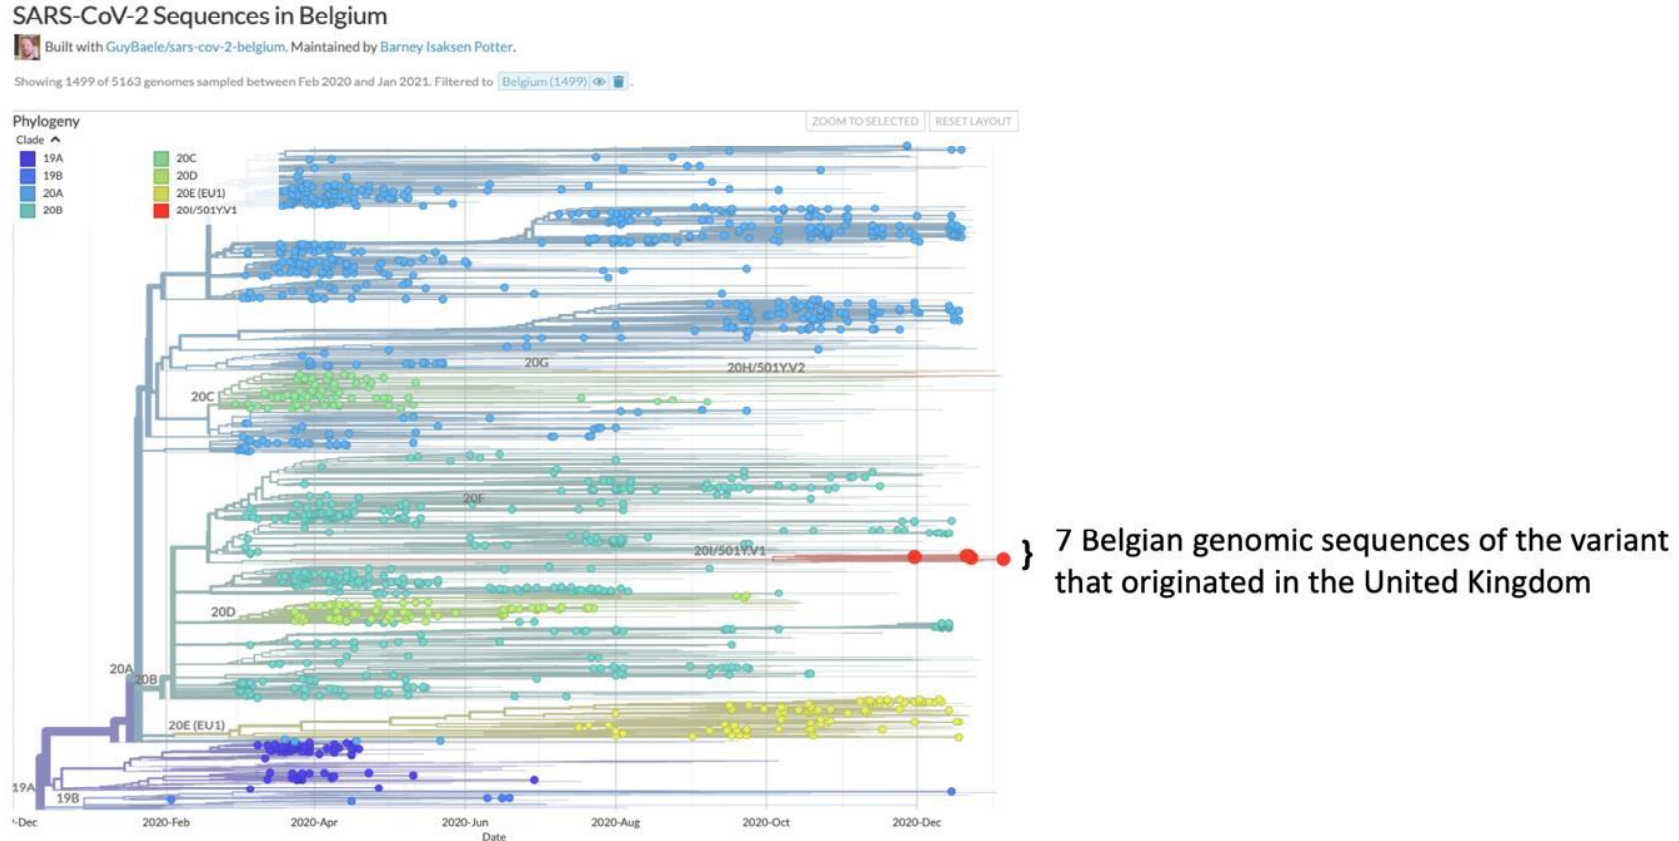
\includegraphics[width=.8\textwidth]{sitRep501YV1}
  \caption[UK variant 501Y.V1 sequenced in Belgium]{UK variant 501Y.V1 sequenced in Belgium.}
  \label{fig:sitRep501YV1}
\end{figure}

\begin{figure}[ht]
  \centering
  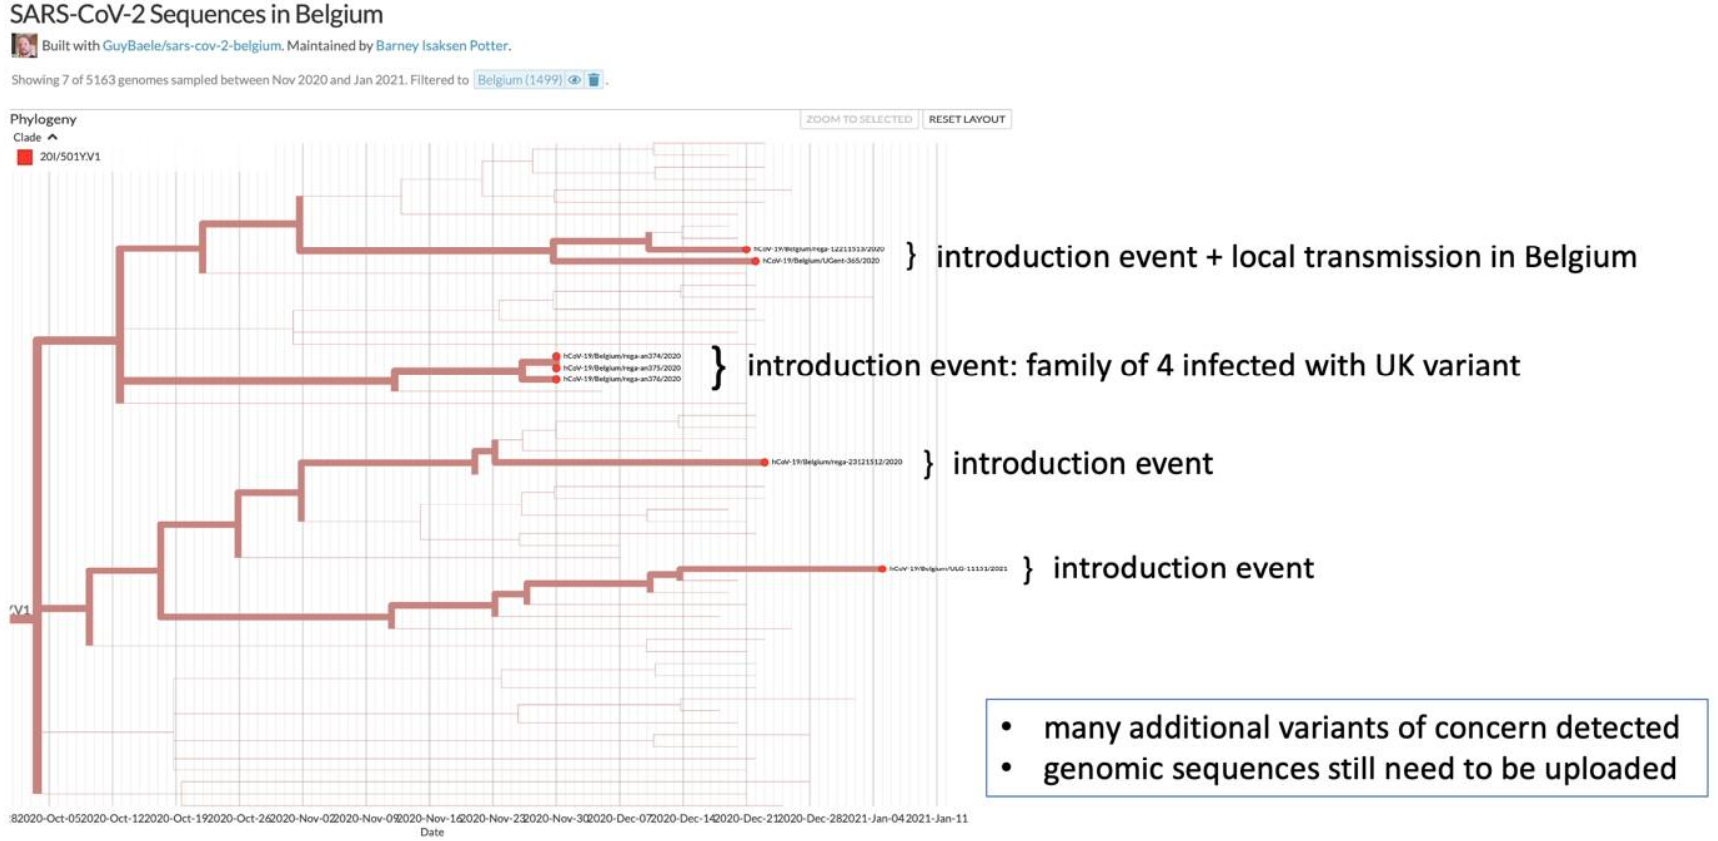
\includegraphics[width=.8\textwidth]{sitRepLocalTransmission}
  \caption[Local transmission in Belgium of UK variant 501Y.V1]{Local transmission in Belgium of UK variant 501Y.V1.}
  \label{fig:sitRepLocalTransmission}
\end{figure}

\subsubsection{Active surveillance through ``S dropouts''}
As shown below, the H69- deletion in the S gene, which generates the ``S dropout'' profile in the \gls{pcr} used by the Belgian Federal Platform Bis laboratories, is not only present in the 501Y.V1, but also in non-\gls{voc} strains circulating in Belgium since several months.
This is the reason why this signal cannot be considered as specific for \gls{voc}s, nor highly sensitive, considering that 501Y.V2 and 501Y.V3 do not present this deletion.

Another element that needs to be considered is that among Platform Bis laboratories, a variable proportion of ``S dropouts'' also show a weak Orf signal (\textit{table not shown}), what has not been typically described with the 501Y.V1.

\vdots

Nevertheless, considering the high number of travels between UK (and Ireland) and Belgium and that this \gls{voc} is already circulating since a number of months in the UK, using the evolution of the proportion of S dropouts among the positive \gls{pcr} results is informative of the current situation in our country.

\begin{figure}[ht]
  \centering
  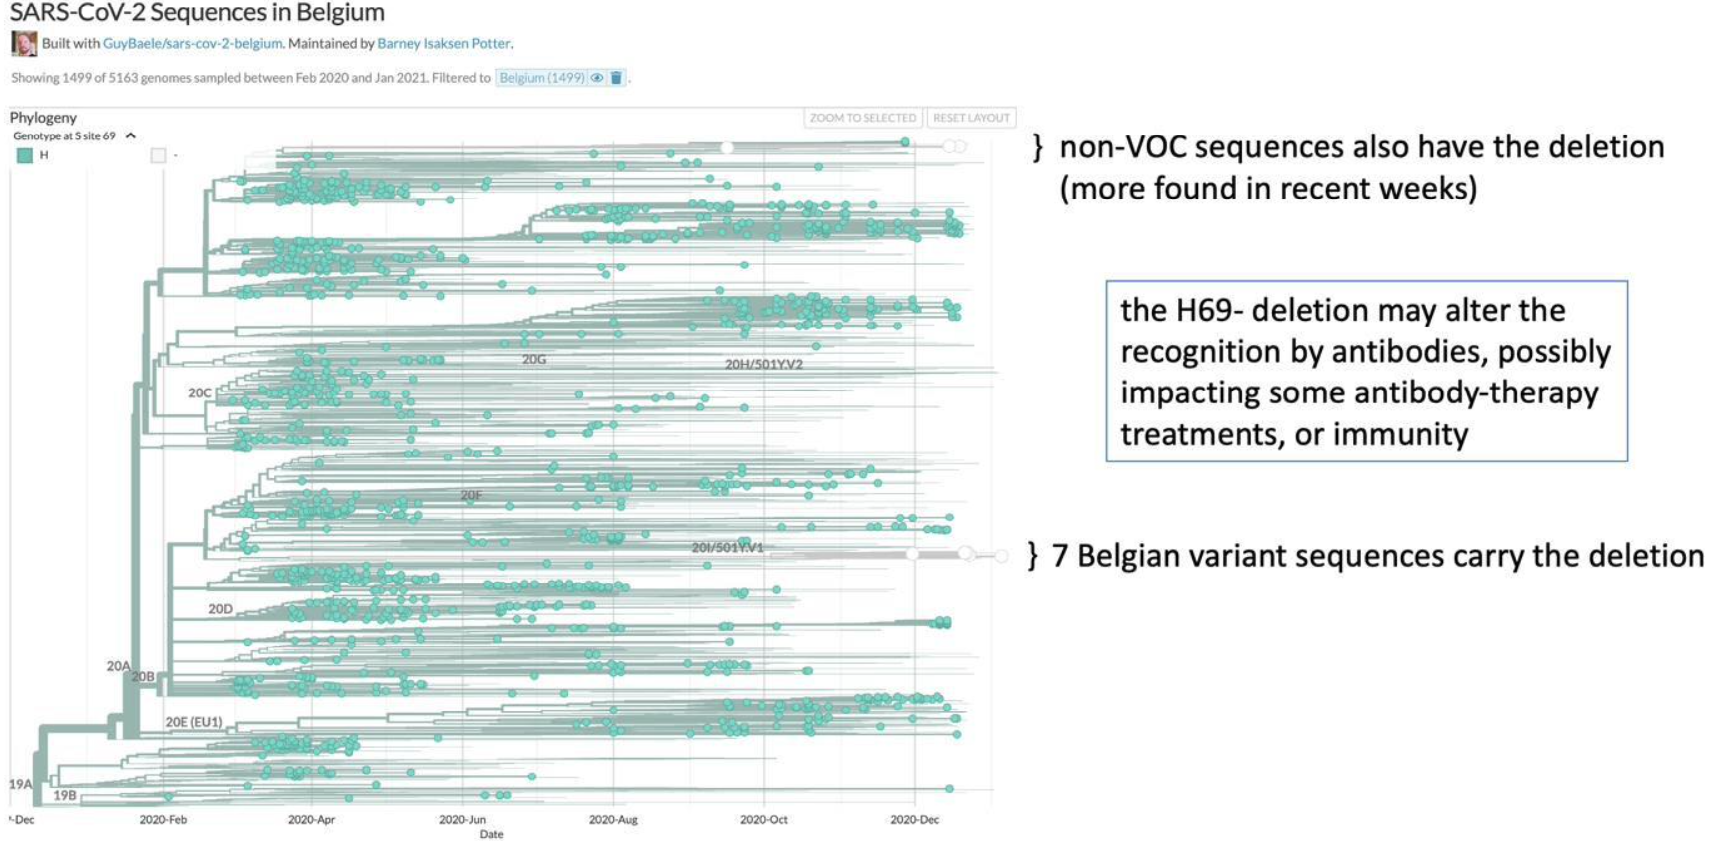
\includegraphics[width=.8\textwidth]{sitRepH69del}
  \caption[Few Belgian sequences with H69- deletion]{Few Belgian sequences with H69- deletion.}
  \label{fig:sitRepH69del}
\end{figure}

\subsection{Baseline surveillance and variants of interest: 18 February 2021}
\subsubsection{Executive summary}
Genomic surveillance in Belgium is organised around 3 different arms aiming to monitor the emergence and the further spread of specific viral populations (variants of concern, \gls{voc}s) which may impact disease control and/or vaccination strategies.

Through ``baseline surveillance'', an unbiased selection of positive samples from 24 sentinel labs (selected based on geographical dispersion and diversity of clinical patterns) are analysed in designated sequencing platforms.
Currently, 5.526 Belgian sequences are available on GISAID. During weeks 5,6 and 7, 728 samples have been sequenced as part of the baseline surveillance, among which 249 were 20I/501Y.V1 (34\%), 30 were 20H/501Y.V2 (4\%) and 3 were 20J/501Y.V3 (0,4\%).
Considering baseline and active surveillance together since Week 1, laboratories positively confirmed the presence of 1.339 \gls{voc}s in Belgium (1.183 20I/501Y.V1, 148 20H/501Y.V2 and 8 20J/501Y.V3).

In this report, we describe a new viral variant consistently detected in Belgium and probably originating from central African countries.
This variant shows a combination of several mutations and deletions which may lead to competitive advantages and would explain why this strain seems to successfully spread in Belgium under the current---and extensive---disease control arsenal.

\subsubsection{International context}
Since the end of the year, 4 variants of concern (\gls{voc}s) have arisen independently of one another in the United Kingdom (20I/501Y.V1), South Africa (20H/501Y.V2) and Brazil (20J/501Y.V3 and P.2).
These variants harbour several mutations and deletions associated with higher infectiousness and immune escape.
All variants are spreading internationally, with 3 \gls{voc}s having been detected to date in Belgium (1.183 for 20I/501Y.V1, 148 for 20H/501Y.V2 and 8 for 20J/501Y.V3).

\subsubsection{Baseline surveillance}
Since support was offered by the federal government end of December 2020, both the temporal coverage (number of sequences performed per week) and geographical coverage (number of collection sites) have improved.
Currently, 5.526 Belgian sequences are available on GISAID.

\vdots

During weeks 5,6 and 7, 728 samples have been sequenced as part of the baseline surveillance, among which 249 were 20I/501Y.V1 (34\%), 30 were 20H/501Y.V2 (4\%) and 3 were 20J/501Y.V3 (0,4\%).

\begin{figure}[ht]
  \centering
  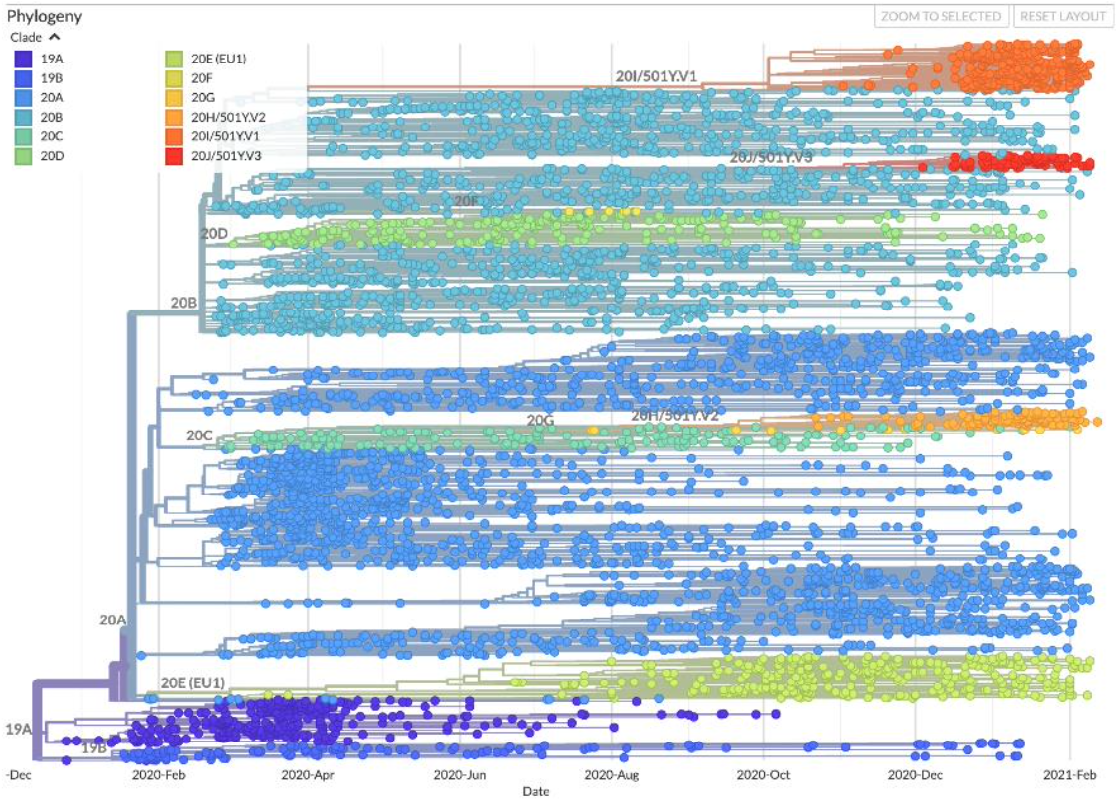
\includegraphics[width=.8\textwidth]{sitRepBaseline}
  \caption[Baseline surveillance VOC phylogeny]{Nextstrain build of currently available sequences from Belgium. \gls{voc}s are highlighted in dark orange (20I/501Y.V1), light orange (20H/501Y.V2) and red (20J/501Y.V3). Warning: this phylogeny tree is not representative is biased due to including all sequenced \gls{voc}s.}
  \label{fig:sitRepBaseline}
\end{figure}

Considering baseline and active surveillance together since Week 1, laboratories positively confirmed the presence of 1.339 \gls{voc}s in Belgium (1.183 20I/501Y.V1, 148 20H/501Y.V2 and 8 20J/501Y.V3).
Currently, all 20J/501Y.V3 strains detected in Belgium seem to be clustered when comparing with other strains detected internationally, in particular in Europe.
Nevertheless, the information collected by health inspectors to date do not allow to find a clear link between all these patients.
This suggests that the cluster is actually much wider than the one described hereunder and that backward contact tracing must be pursued and intensified in order to contain this emerging chain of transmission.

\begin{figure}[ht]
  \centering
  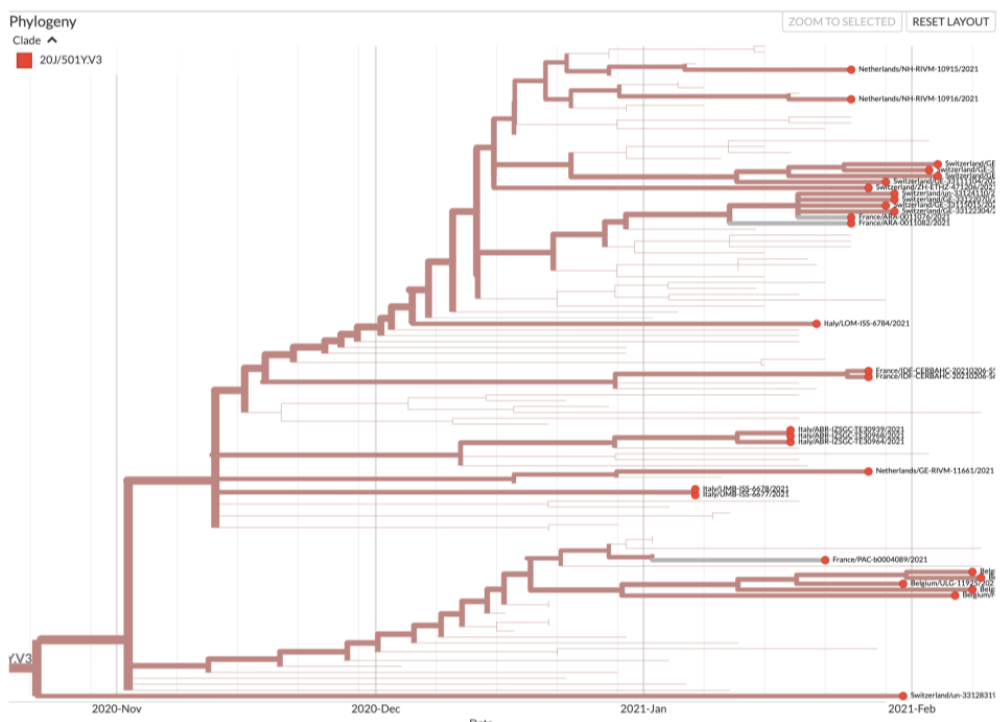
\includegraphics[width=.8\textwidth]{sitRepGamma}
  \caption[20J/501Y.V3 monitoring]{Currently, it the 8 20J/501Y.V3 strains detected in Belgium seem to be clustered when comparing with other strains detected internationally, in particular in Europe. Nevertheless, the information collected by health inspectors to date do not allow to find a clear link between all these patients. This suggests that the cluster is actually much wider than the one described hereunder and that backward contact tracing must be pursued and intensified in order to contain this emerging chain of transmission.}
  \label{fig:sitRepGamma}
\end{figure}

\subsubsection{Variant of interest B1.525}
This variant of interest was first described mid-December in England (England/CAMC-C769B3/2020) and has since then been described in 11 countries: England (28), Nigeria (7), USA (7), France (5), Canada (4), Ghana (4), Japan (4), Jordan (2), \textbf{Belgium (1)}, Italy (1) and Spain (1).

This variant is characterised by mutations: S:E484K, S:Q677H, S:F888L, S:69-70 deletion, and S:144 deletion, and a 9 nucleotide mutation in nsp6 (as seen in B.1.1.7, B.1.351, P.1). (\url{https://github.com/cov-lineages/pango-designation/issues/4}).

\subsubsection{Variant of interest with Spike Insertion (VOI-SI)}
A key feature of the recently identified \gls{voc}s is a suite of single base pair mutations that generate amino acid changes at key points within the spike protein.
In addition to these single base pair changes, a number of sometimes overlapping short deletions have been observed in the different \gls{voc}s \citep{garry2021spike}, both within spike and other viral genes \citep{pango4}.

The lineage B.1.1.7 (20I/501Y.V1), which arose in the United Kingdom in late 2020 \citep{rambaut2020preliminary} and the recently described B.1.525 lineage \citep{pango4}, carry deletions in spike affecting amino acid positions 69-70 & 144, while the B.1.351 lineage (20H/501Y.V2), originally identified in South Africa \citep{Tegally2020} carries a deletion of three amino acids (positions 242 to 244) in spike.
In contrast, the P.1 lineage (20J/501Y.V3) \citep{faria2021genomic} does not carry any deletions in the spike protein, however, all four carry a three amino acid deletion in the nsp6 protein.

In contrast to spike deletions, the frequency of insertions in the SARS-CoV-2 spike gene appears rare. \citet{garry2021spike} examined ~350,000 SARS-CoV-2 sequences from the GISAID database, identifying only two examples with insertions at amino acid R214.
In the same report they also point out that passage of SARS-CoV-2 in cell culture (Vero cells) can generate amino acid insertions in the same spike region \citep{garry2021spike}, indicating that in some contexts such insertions are advantageous.

\begin{figure}[ht]
  \centering
  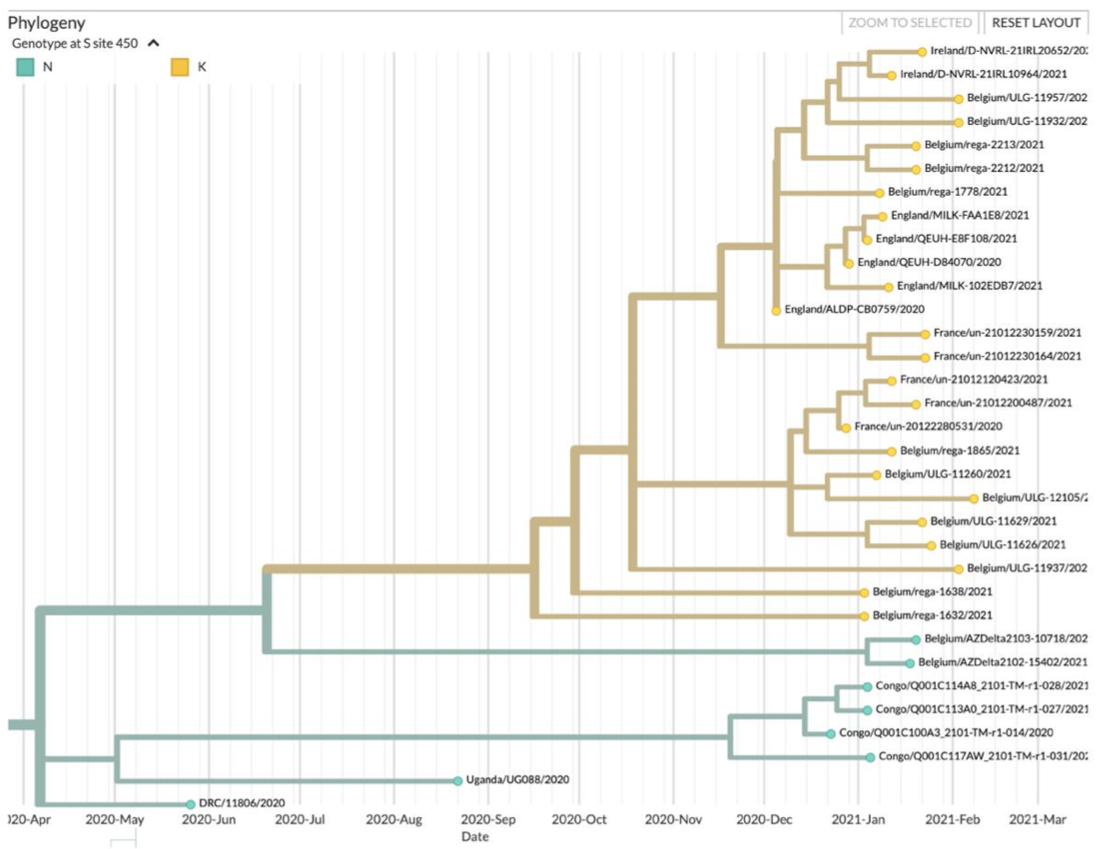
\includegraphics[width=.8\textwidth]{voiSI}
  \caption[VOI-SI monitoring]{\gls{voi}-SI which also harbour the N450K amino acid change (shown in yellow) cluster together, the Belgian samples fall across the cluster indicating multiple independent introductions.}
  \label{fig:voiSI}
\end{figure}

Baseline surveillance of SARS-CoV-2 genomes carried out at the University of Li\`{e}ge highlighted a Belgian genome carrying a spike insertion, which we will refer to as Variant of Interest with Spike Insertion (\gls{voi}-SI).
The sample was collected on the \nth{7} January, in an individual hospitalised for COVID-19, who recently returned from travel in the Congo.
In the subsequent weeks additional similar genomes have been identified by both ULi\`{e}ge and UZ Leuven/KU Leuven, while genomes from the same lineage have been deposited in the GISAID database with origins in the UK, Ireland and France.

The earliest example of a \gls{voi}-SI was isolated in the UK on the \nth{5} of December and was one of the spike insertions identified by \citet{garry2021spike}.
To date that number has grown to 43, with the majority (30) isolated in Belgium.
The Pangolin COVID-19 Lineage Assigner (\url{https://pangolin.cog-uk.io/}) assigns the majority of the \gls{voi}-SI to lineage B.1.214 which is most commonly found in the Democratic Republic of the Congo.
A Nextrain [\textit{sic}] build using the available \gls{voi}-SI shows them to cluster together and indicates that the lineage has been introduced to Belgium multiple times (Fig.~\ref{fig:voiSI}).

In addition to the insertion in spike the lineage also carries a number of other amino acid changes in spike (Q414K, N450K, D614G, T716I) as well as a 30bp deletion in ORF3a (I20-, K21-, D22-, A23-, T24-, P25-, S26-, D27-, F28-, V29-).
This lineage does not have the N501Y or E484K, changes found in the majority of \gls{voc}s, although the T716I amino acid change is also found in the B.1.1.7 lineage.
One of the main reasons for concern regarding the B.1.351, P.1 and B.1.525 lineages is the presence of E484K which has been shown to impact antibody binding \citep{Greaney2021}.
The same work highlighted that mutation in the 443--450 loop region can have a large impact on antibody binding \citep{Greaney2021}, which makes the N450K change observed in the \gls{voi}-SI concerning.

\begin{figure}[ht]
  \centering
  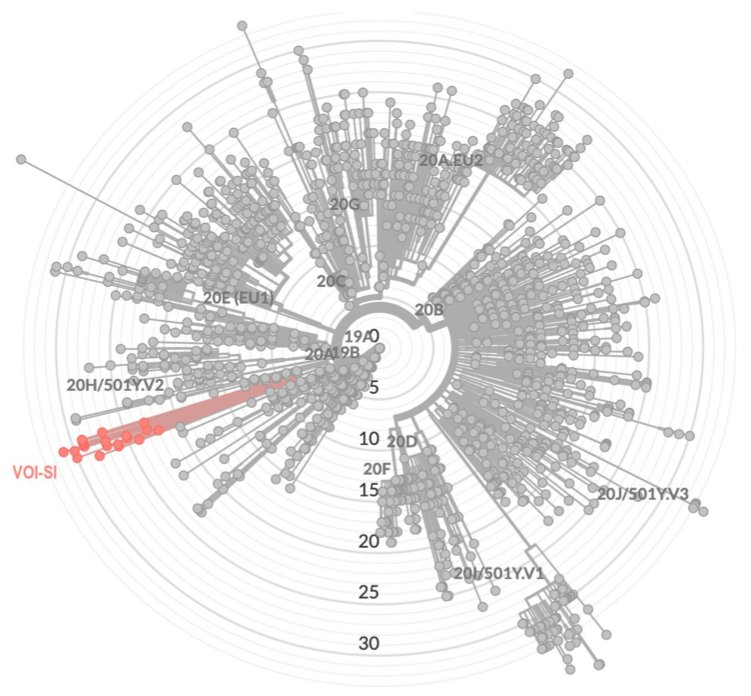
\includegraphics[width=.8\textwidth]{voiSI2}
  \caption[VOI-SI clade]{\gls{voi}-SI forms a separate clade among international SARS-CoV-2 sequences.}
  \label{fig:voiSI2}
\end{figure}

Finally, nearly half of the \gls{voi}-SI genomes submitted to date carry a three amino acid deletion in nsp6.
The same deletion is observed in the \gls{voc} lineages B.1.1.7, B.1.351, B.1.525 and P.1, suggesting epistatic interactions between this deletion and changes in spike.

\subsection{Delta ascendant: 29 June 2021}
\subsubsection{Executive summary}

28.058 Belgian sequences of SARS-CoV-2 are now publicly available on GISAID.
Among these, 486 sequences of positive SARS-CoV-2 samples collected between 14 June and 27 June were reported,
\begin{itemize}
  \item B.1.1.7 (Alpha) represented 65,2\% (compared to 71,3\% in the last report)
  \item B.1.617.2 (Delta) represented 23\% (compared to 15,7\% in the last report)
  \item P.1 (Gamma) represented 8,6\% (compared to 9,7\% in the last report)
  \item B.1.351 (Beta) represented 0,8\% (compared to 1,2\% in the last report)
\end{itemize}

Other points of attention:
\begin{itemize}
  \item The NRC performed 63 \gls{voc} \gls{pcr}s on unselected positive samples analyzed during the last 9 days.
B.1.1.7 and B.1.617.1/.2 represented respectively 33,3\% and 60,3\% of the results.
  \item The decreasing epidemiological trend observed in Belgium is a very positive element as it will help
mitigate the impact of the rapid viral population replacement currently taking place.
\end{itemize}

Currently, the absolute number of B.1.617.2 cases reported is not rising.
This fragile equilibrium could be disrupted and lead to a deterioration of the epidemiological situation by a combination of (1) relaxation of measures, (2) an increasing number of travellers that will return from zones where the number of infections is rapidly increasing and (3) the foreseen limited coverage of testing offered to travellers coming back from red zones, resulting in a higher risk of secondary infections after importation of cases.

\subsubsection{Monitoring of \gls{voc}s}
\paragraph*{International evolution.}
The Delta variant (B.1.617.2) has continued to spread globally.
It has become the dominant lineage in several European countries, and other EU countries are expected to follow this evolution during the summer period.

\vdots

\paragraph*{Situation in Belgium.}
While it was first identified on 6 April 2021 in Belgium, the B.1.617.2 Variant of Concern (Delta) is on its path to become the dominant lineage in the country.
Between 14/6/2021 and 27/6/2021 (486 genomes available to date):
\begin{itemize}
  \item B.1.1.7 (Alpha) represented 65,2\%
  \item B.1.617.2 (Delta) represented 23\%
  \item P.1 (Gamma) represented 8,6\%
  \item B.1.351 (Beta) represented 0,8\%
\end{itemize}

\begin{figure}[ht]
  \centering
  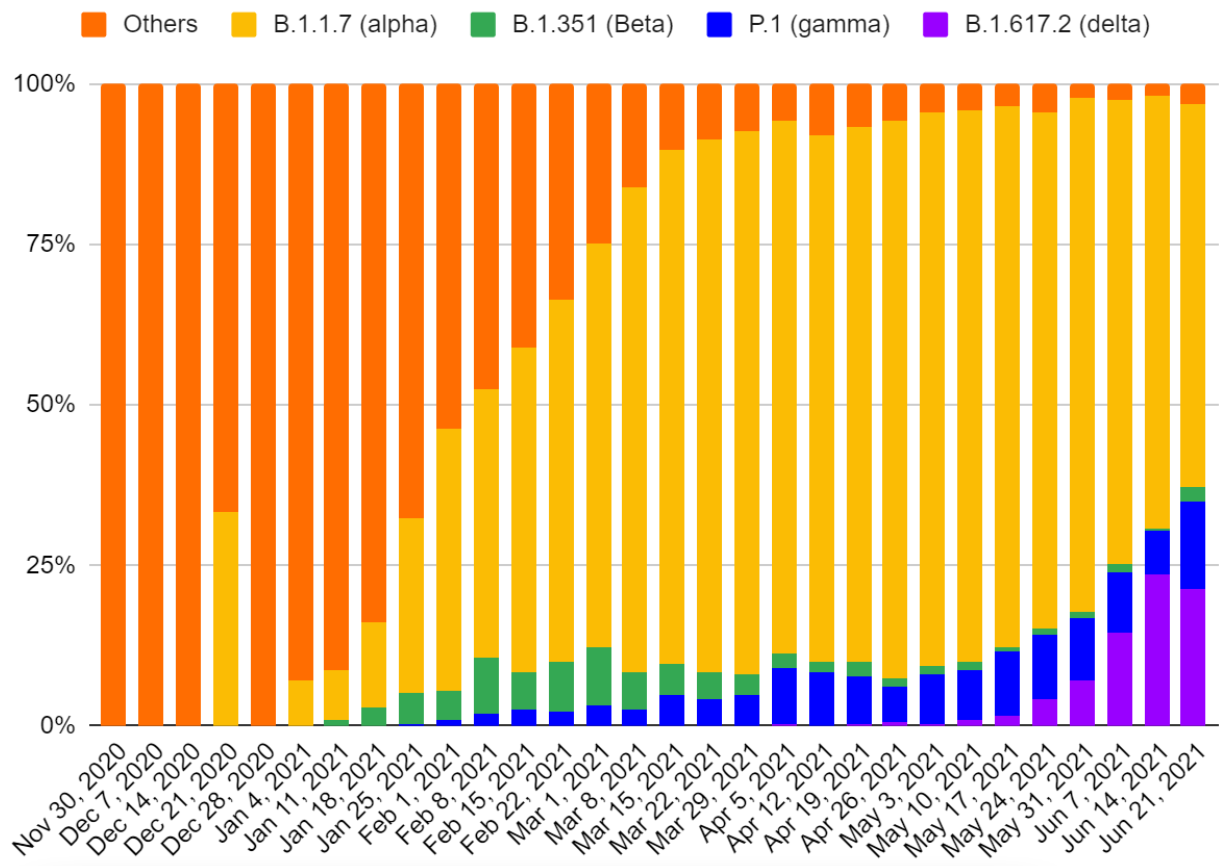
\includegraphics[width=.8\textwidth]{deltaFreq}
  \caption[Weekly VOCs as of 2021-06-21]{Weekly evolution of the frequency of variants of concern reported by the baseline surveillance network using a whole genome sequencing (WGS) approach.}
  \label{fig:deltaFreq}
\end{figure}

\vdots

\begin{figure}[ht]
  \centering
  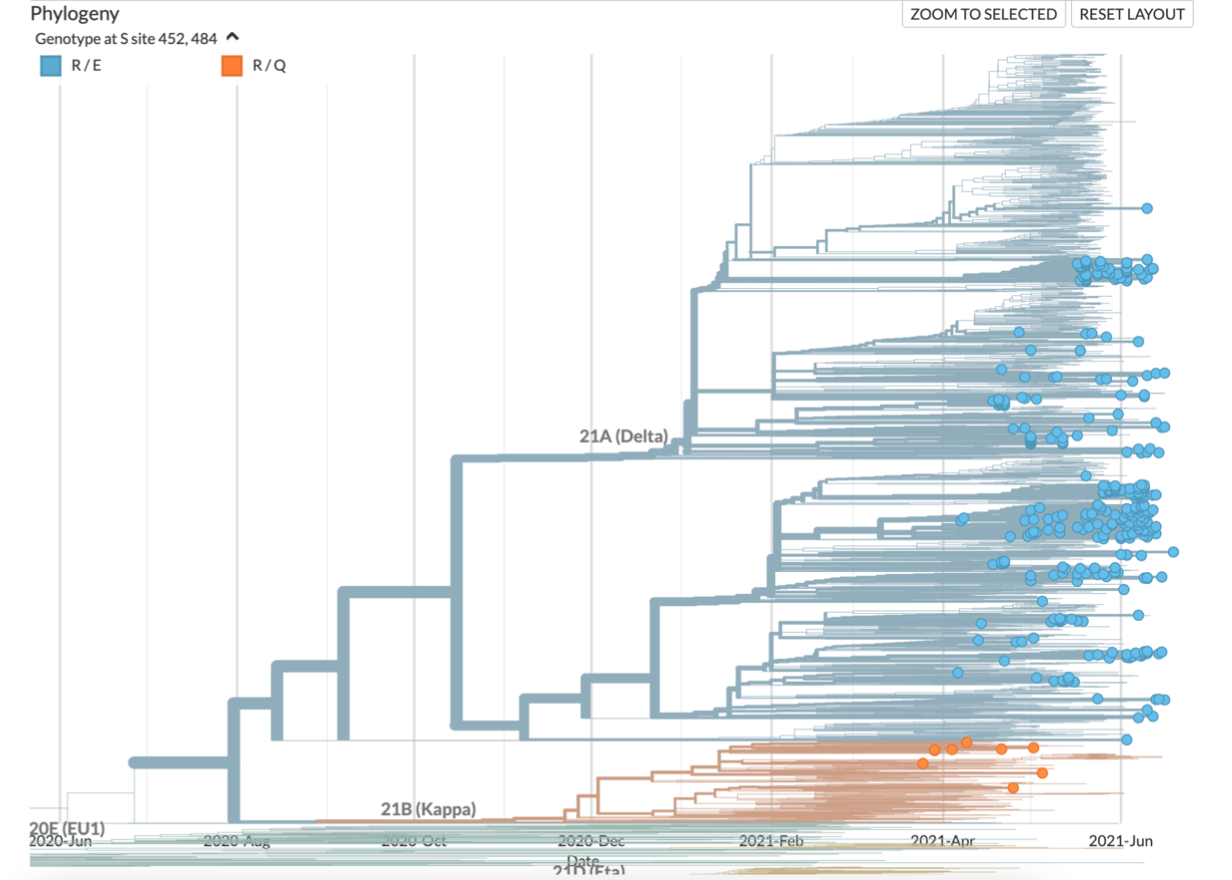
\includegraphics[width=.8\textwidth]{deltaIntro}
  \caption[Introductions and local transmission of B.1.617.2]{381 Belgian genomes in the latest available Nextstrain build show both small and large local transmission clusters within Belgium for B.1.617.2.}
  \label{fig:deltaIntro}
\end{figure}

\begin{figure}[ht]
  \centering
  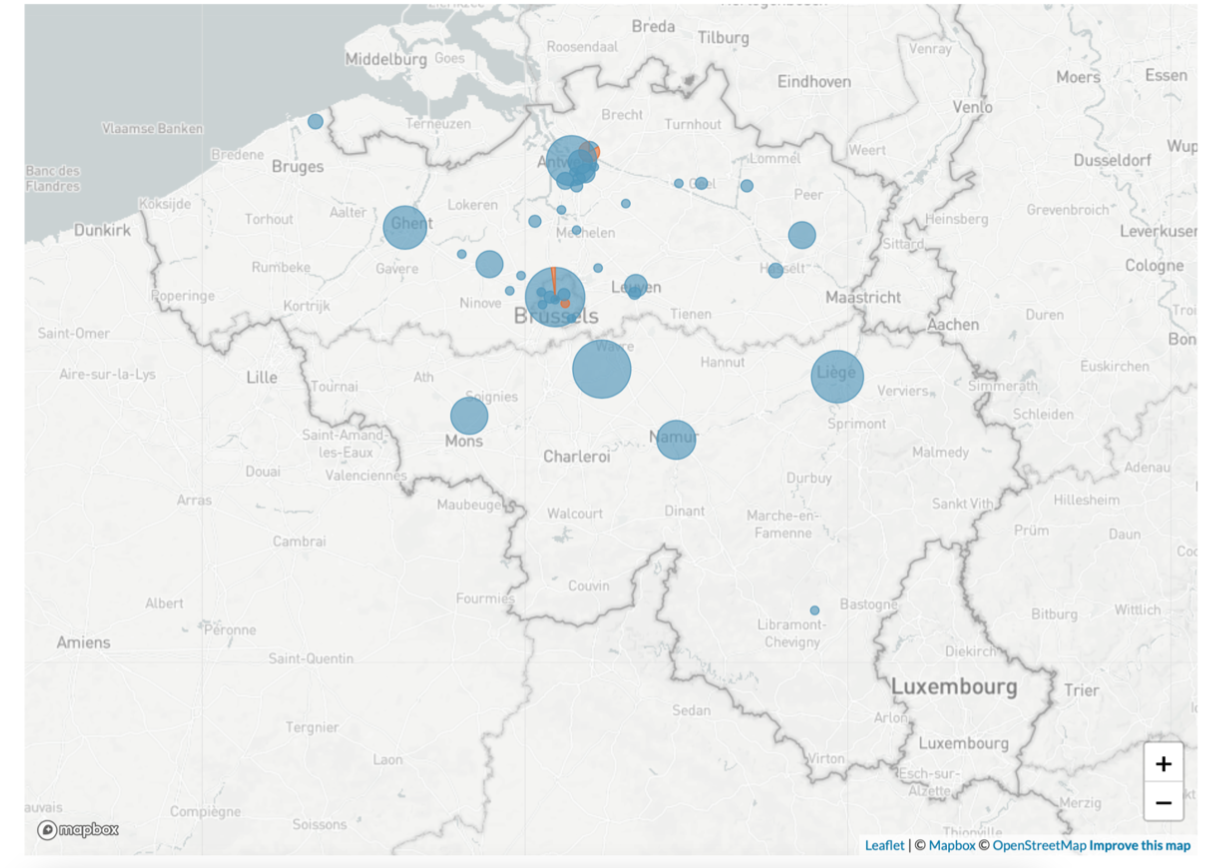
\includegraphics[width=.8\textwidth]{deltaDist}
  \caption[Distribution of Belgian B.1.617.2 sequences]{B.1.617.2 is present in all Belgian provinces but mostly in and around major cities.}
  \label{fig:deltaDist}
\end{figure}

Two large clades of B.1.617.2 can be seen in Figure~\ref{fig:deltaIntro}. In Figures~\ref{fig:delta1}~and~\ref{fig:delta2}, we look into each of those clades in more detail, focusing on the possible relationship between the situation in Belgium and the United Kingdom.

Whereas Figure~\ref{fig:delta1}, showing less than half of the Belgian B.1.617.2 genomes (the upper blue part in Figure~\ref{fig:deltaIntro}), indicates the importance of our connection to/with the United Kingdom, Figures~\ref{fig:delta2}~and~\ref{fig:delta3} (showing the majority of Belgian infections; the lower blue part in Figure~\ref{fig:deltaIntro}) paint a somewhat different picture.
While some infections and local transmission clusters in Belgium can still be linked to the United Kingdom (see Figure~\ref{fig:delta2}), Figure~\ref{fig:delta3} shows the impact of Asian countries (India, Singapore, ...) on the increase of B.1.617.2 infections in Belgium.

\begin{figure}[ht]
  \centering
  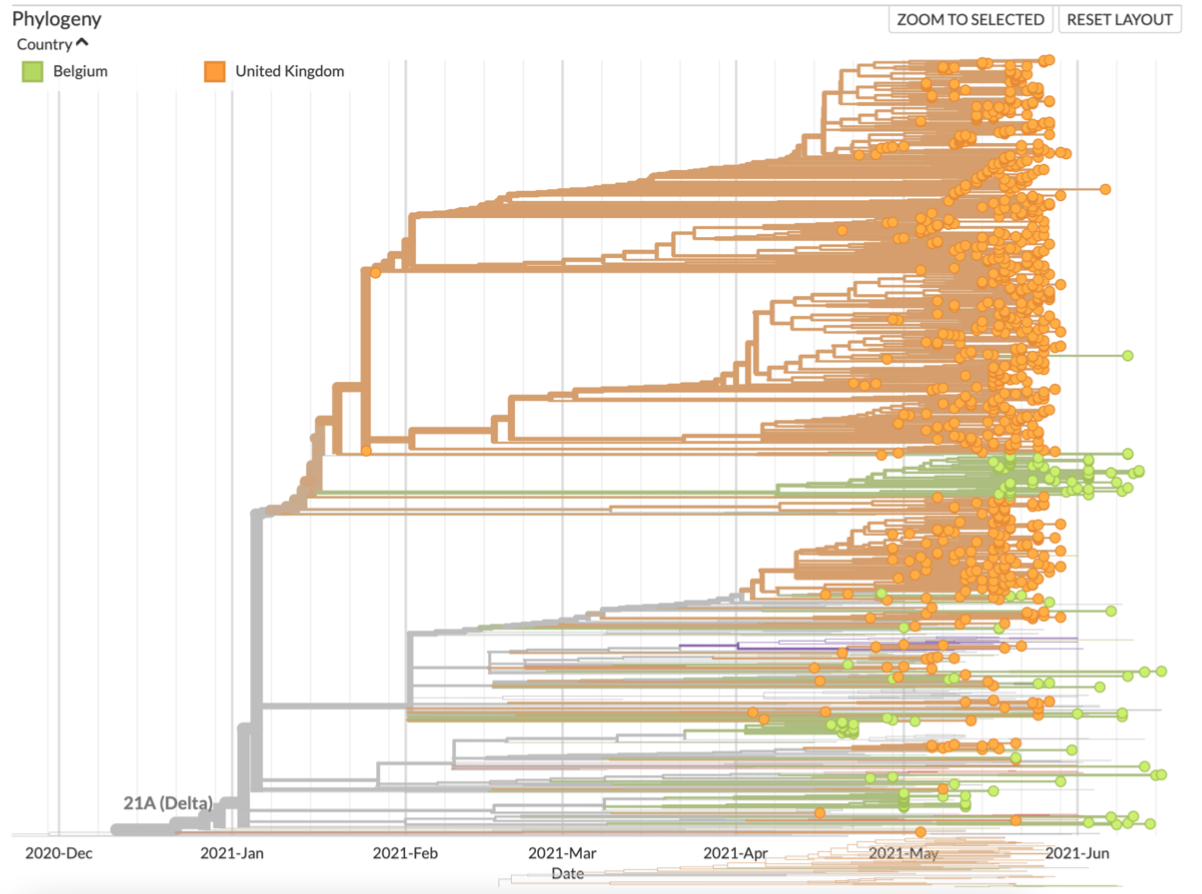
\includegraphics[width=.8\textwidth]{delta1}
  \caption[B.1.617.2 clade 1]{Top clade in Figure~\ref{fig:deltaIntro} analysed in more detail (orange: United Kingdom; green: Belgium). The largest (transmission) cluster of infections is nested within an otherwise entirely UK clade, suggesting the role of the UK in seeding a proportion of B.1.617.2 introductions into Belgium, in a similar manner as to what was observed at the time of B.1.1.7. Single-case introductions and smaller transmission clusters in Belgium can be seen to have both a UK and a non-UK origin.}
  \label{fig:delta1}
\end{figure}

\begin{figure}[ht]
  \centering
  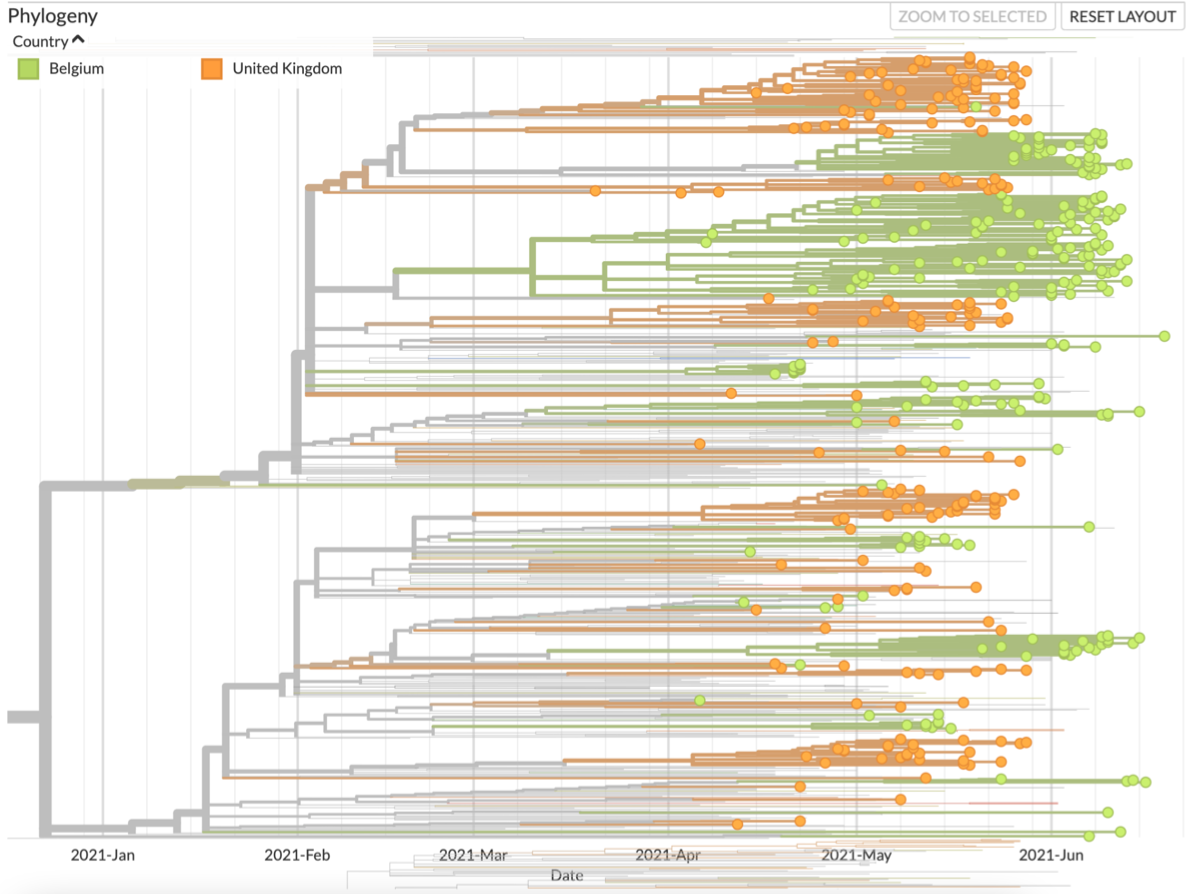
\includegraphics[width=.8\textwidth]{delta2}
  \caption[B.1.617.2 clade 2]{Bottom clade in Figure~\ref{fig:deltaIntro} analysed in more detail (orange: United Kingdom; green: Belgium), showing---to a lesser extent as in Figure~\ref{fig:delta1}---the importance of the situation in the UK for Belgium.}
  \label{fig:delta2}
\end{figure}

\begin{figure}[ht]
  \centering
  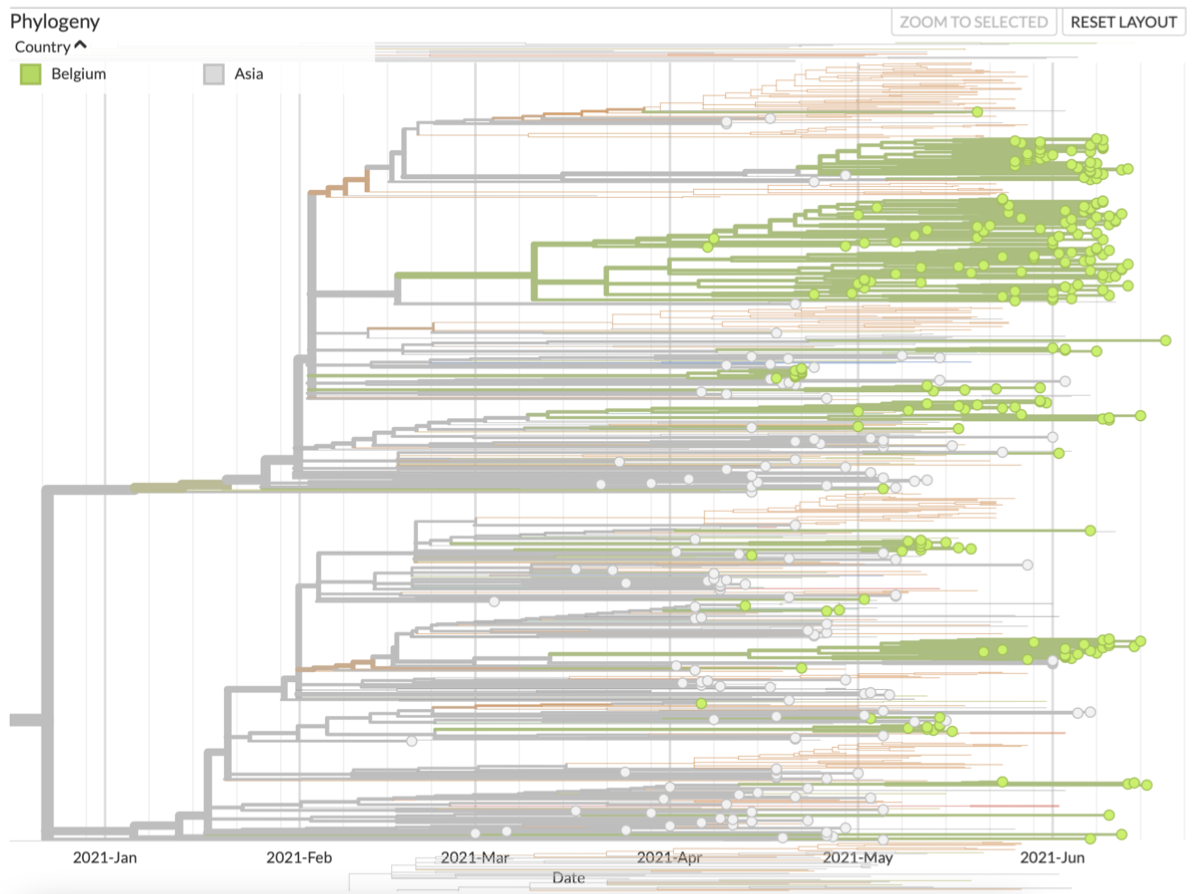
\includegraphics[width=.8\textwidth]{delta3}
  \caption[B.1.617.2 alternate coloring]{Alternative representation of Figure~\ref{fig:delta2} to assess the relationship between Asian countries and Belgium, showing the importance of introductions from those countries into Belgium.}
  \label{fig:delta3}
\end{figure}

\section{Two years of genomic surveillance in review}\label{sec:twoYears}

\singlespacing
\hrule
\vspace*{12pt}
The following was published as \textbf{Lize Cuypers, Simon Dellicour, Samuel L Hong, Barney I Potter, Bruno Verhasselt, Nick Vereecke, Laurens Lambrechts, Keith Durkin, Vincent Bours, Sofieke Klamer, Guillaume Bayon-Vicente, Carl Vael, Kevin K Ari\"{e}n, Ricardo De Mendonca, Oriane Soetens, Charlotte Michel, Bertrand Bearzatto, Reinout Naesens, Jeremie Gras, Anne Vankeerberghen, Veerle Matheeussen, Geert Martens, Dagmar Obbels, Ann Lemmens, Bea Van den Poel, Ellen Van Even, Klara De Rauw, Luc Waumans, Marijke Reynders, Jonathan Degosserie on behalf of COVID-19 Genomics Belgium Consortium, Piet Maes, Emmanuel Andr\'{e}, Guy Baele}.
``Two years of genomic surveillance in Belgium during the SARS-CoV-2 pandemic to attain country-wide coverage and monitor the introduction and spread of emerging variants.'' \textit{Viruses} 14, no.
10 (2022): 2301.

The efforts made by the entirety of the COVID-19 Genomics Belgium consortium\footnote{Membership of the COVID-19 Genomics Belgium Consortium is listed in the Acknoledgments of this chapter.} represent a herculean, multidisciplinary effort to use genomic epidemiology to try to mitigate the effects of the COVID-19 epidemic in Belgium.
This included front-line clinicians, wet lab scientists, modelers, data scientists, and numerous researchers willing to put themselves on in the path of not only the virus itself, but also into the public and political spotlight.
The publication that follows represents a collaborative, \textit{post hoc} review of just a fraction of the total effort that was put forth by so many people to combat the pandemic.

In addition to the public-facing Nextstrain instance mentioned in Section~\ref{sec:nextstrainBE}, and genomic surveillance reports mentioned in Section~\ref{sec:sitRep}, which are in part summarized below, I performed sampling and preliminary ML analysis for several of the published research articles mentioned herein.
\vspace*{12pt}
\hrule
\onehalfspacing

\subsection{Introduction}
The continued accumulation of \gls{sarscov2} infections across the world keeps posing significant threats to public health.
Since the start of the pandemic, many countries sought to avoid or control a next wave of infections using non-pharmaceutical interventions (including social distancing, mask wearing and partial or complete lockdowns) to avoid flooding hospitals with patients and to keep medical care facilities from collapsing.
The key motivation behind many of these measures was to guarantee high-quality health care and limit delays to essential treatments (e.g., surgery, chemotherapy and/or radiation therapy) for all patients.
After an initial wave of infections in 2020, countries sought to find a balance between the impact of the imposed preventative measures on economic and social activities, and the often severe and potentially long-term impact of COVID-19 on public health (e.g., long COVID), and economic and social activities \citep{zivin2020spread}.
Since the end of 2020, vaccination campaigns have been deployed around the world, and an increasing number of vaccines continues to be approved by public health authorities, while ongoing research efforts monitor the evolution and spread of \gls{sarscov2} at both national and international levels.

In the midst of combating the pandemic, the repeated emergence of new mutations of the \gls{sarscov2} genome in different countries has been and still is a cause for concern.
Accumulation of mutations is a natural consequence of the abundant replication of the virus worldwide, and it is to be expected that a subset of these mutations is progressively selected, leading to the emergence of new variants.
Such emerging variants might harbor advantages with regard to transmissibility, immune escape and/or other fitness features in comparison to other circulating strains, and they are therefore to be carefully monitored and evaluated.
The D614G mutation on the spike protein was the first mutation suspected to lead to a higher transmissibility of \gls{sarscov2}.
Rarely occurring before March 2020, this mutation became increasingly common as the pandemic spread, occurring in over 74\% of all published sequences by June 2020 \citep{korber2020tracking,plante2021spike}.
Although this variant nearly completely replaced the original Wuhan variant, it is still debated as to whether this mutation did indeed lead to increased transmissibility, with certain studies having suggested only a moderate impact on transmissibility \citep{cogUKreport1,volz2021evaluating}.

In late 2020, the UK faced a rapid increase in COVID-19 cases in South East England, leading to enhanced epidemiological and virological investigations \citep{cogUKreport1}, which revealed a novel \gls{sarscov2} variant, now referred to as Alpha (lineage B.1.1.7).
This variant was defined by a set of 23 mutations, 14 amino acid changes and three deletions, compared to the original Wuhan isolate.
Most notably, the N501Y mutation and the HV 69--70 deletion are present in lineage B.1.1.7 \citep{rambaut2020dynamic}, which had been growing in frequency since November 2020.
Preliminary analyses in the UK rapidly suggested that this variant was significantly more transmissible than previously circulating variants, with an estimated potential to increase the effective reproductive number ($R_e$) by a value ranging between 0.4 and 0.7 \citep{volz2021assessing}.

The \gls{sarscov2} variant of concern (\gls{voc}) Alpha (lineage B.1.1.7) was identified using a broad high-throughput sequencing (HTS) strategy implemented in the UK, where up to 10\% of all \gls{sarscov2} \gls{pcr}-positive samples were being sequenced at the time.
This strategy also enabled the UK to detect two cases of the Beta \gls{voc} (lineage B.1.351), which was first detected in South Africa.
Impacting mostly southern African countries and defined by eight mutations in the spike protein, including three substitutions (K417N, E484K and N501Y) at residues in its receptor-binding domain that may have functional importance, Beta showed rapid expansion and displacement of other lineages in several regions \citep{tegally2021detection}.
However, the impact of this \gls{voc} in Belgium remained rather limited compared to the other \gls{voc}s.

First detected in Brazil, and quickly following in the footsteps of Beta (lineage B.1.351), the Gamma \gls{voc} (lineage P.1) was characterized by 17 mutations, including a trio of mutations in the spike protein (K417T, E484K, and N501Y) associated with increased binding to the human ACE2 (angiotensin-converting enzyme 2) receptor.
\citet{faria2021genomics} estimated that P.1 may have been 1.7 to 2.4 times more transmissible than local non-P.1 lineages, and that previous (non-P.1) infection provides 54 to 79\% of the protection against infection with P.1 than it provides against non-P.1 lineages.
The Gamma \gls{voc} mostly affected southern American countries, but, like Beta, had only limited impact on the pandemic situation in Belgium.

Starting its rise to become the global dominant lineage in April 2021, the Delta \gls{voc} (lineage B.1.617.2) was first detected in India and bears the L452R spike receptor-binding motif (RBM) substitution, previously reported to confer increased infectivity and a modest loss of susceptibility to neutralizing antibodies.
\citet{mlcochova2021sars-cov-2} found that increased replication fitness and reduced sensitivity of \gls{sarscov2} B.1.617.2 to neutralizing antibodies contributed to the rapid increase in B.1.617.2 cases, compared to B.1.1.7 and other lineages.
The authors also demonstrated the evasion of neutralizing antibodies by a B.1.617.2 live virus with sera from convalescent patients, as well as sera from individuals vaccinated with two different vaccines, and reported vaccine breakthrough infections in healthcare workers in three hospitals, demonstrating reduced vaccine effectiveness against B.1.617.2.

Since mid-January 2022, the Omicron \gls{voc} (lineage B.1.1.529/BA.1) has become the dominant lineage in most countries worldwide, with a growing tendency to displace lineage B.1.617.2.
Having been detected in November 2021 by genomic surveillance teams in South Africa and Botswana, the Omicron \gls{voc} carries over 30 mutations in the spike glycoprotein, which \citet{martin2022selection} predicted would influence antibody neutralization and spike function.
\citet{viana2022rapid} were the first to describe the genomic profile and early transmission dynamics of Omicron, showing rapid spread of the Omicron \gls{voc} in regions with high levels of population immunity.

The continued emergence of novel \gls{sarscov2} lineages and \gls{voc}s is testament to the importance of performing adequate genomic surveillance in countries around the world.
Toward the end of 2020, the \gls{ecdc} emphasized the reinforcement of HTS to facilitate the detection of these and (re-)emerging variants \citep{ecdcSequencing}.
Sample collection should aim for a robust representation of the population (geographic distribution, age groups, etc.) to create a representative baseline surveillance, but could also have a focus on areas or populations associated with a rapid increase in incidence or reports of increased severity.
The \gls{ecdc} and the WHO further insisted that member states deposit their sequences to the international database GISAID \citep{shu2017gisaid} to make them available to the entire scientific community \citep{ecdcSequencing}.
Additionally, associated metadata should be shared and annotated in a consistent manner to facilitate analyses and accompanying visualization.
Already, in 2020, the \gls{ecdc} offered their member states a case-based reporting system for the reporting of genomic \gls{sarscov2} results, with a focus on the emerging \gls{voc}s, coupled with epidemiologic COVID-19 case-based reporting through national public health institutes.

As a result, and starting in 2021, countries around the world intensified their efforts toward genomic surveillance in order to detect and monitor the co-circulating \gls{voc}s Alpha, Beta, Gamma \citep{greaney2021comprehensive}, Delta and Omicron in their population, recognizing the need for ongoing and continuous sequencing during the \gls{sarscov2} pandemic \citep{martin2021insights}.
We here describe the genomic surveillance efforts in Belgium, both before and after the establishment of a nationwide genomic surveillance consortium.
We first discuss project-based research efforts from before systematic funding for whole-genome sequencing (WGS) became available, followed by the structure and workflow of the Belgian genomic surveillance consortium.
These efforts opened up many opportunities for joint projects and research studies, which we discuss in the respective sections below.


\subsection{Prior to the National Genomic Surveillance Initiative}
In 2020, \gls{sarscov2} sequencing efforts in Belgium were still largely research-oriented, as no dedicated funding (from the federal government) had been reserved for genomic surveillance efforts.
Within the Flemish Region, two general COVID-19 funding calls were launched during 2020, totaling EUR 2.5 million each, to be distributed among ten research projects.
However, the eligible research projects were a mix of social, economic, and public health applications, all competing with vaccine research and genomic sequencing projects.
Within the Wallonia-Brussels Federation, one call for Exceptional Research Projects (PER) Coronavirus and another for Urgent Research Credits (CUR) Coronavirus were both launched in 2020, but no dedicated funding was set aside for genomic sequencing here either.
As a result, only two \gls{sarscov2} sequencing projects were granted within Belgium (one in the Flemish Region, and one in the Wallonia-Brussels Federation) during 2020, which resulted in different coexisting sampling strategies: UZ/KU Leuven (acting as part of the National Reference Center—NRC—for Respiratory Pathogens) collected samples from all over the country, while the University of Li\`{e}ge focused on samples originating from the province of Li\`{e}ge, the University of Ghent on samples from the provinces of East and West Flanders, and the Institute of Tropical Medicine Antwerp on samples from the province of Antwerp.
This biased sampling strategy is apparent when visualizing a large number of the publicly available Belgian sequences in GISAID (see Fig.~\ref{fig:beGenomesPer10k}).
As a result, Fig.~\ref{fig:beGenomesPer10k} shows clear geographical gaps in Belgium's spatial sequencing coverage during the first year of the pandemic, on top of a lack of temporal continuity, both being the consequences of project-based funding and a non-centralized approach to \gls{sarscov2} genomic surveillance efforts.

% Figure 1
\begin{figure}[ht]
  \centering
  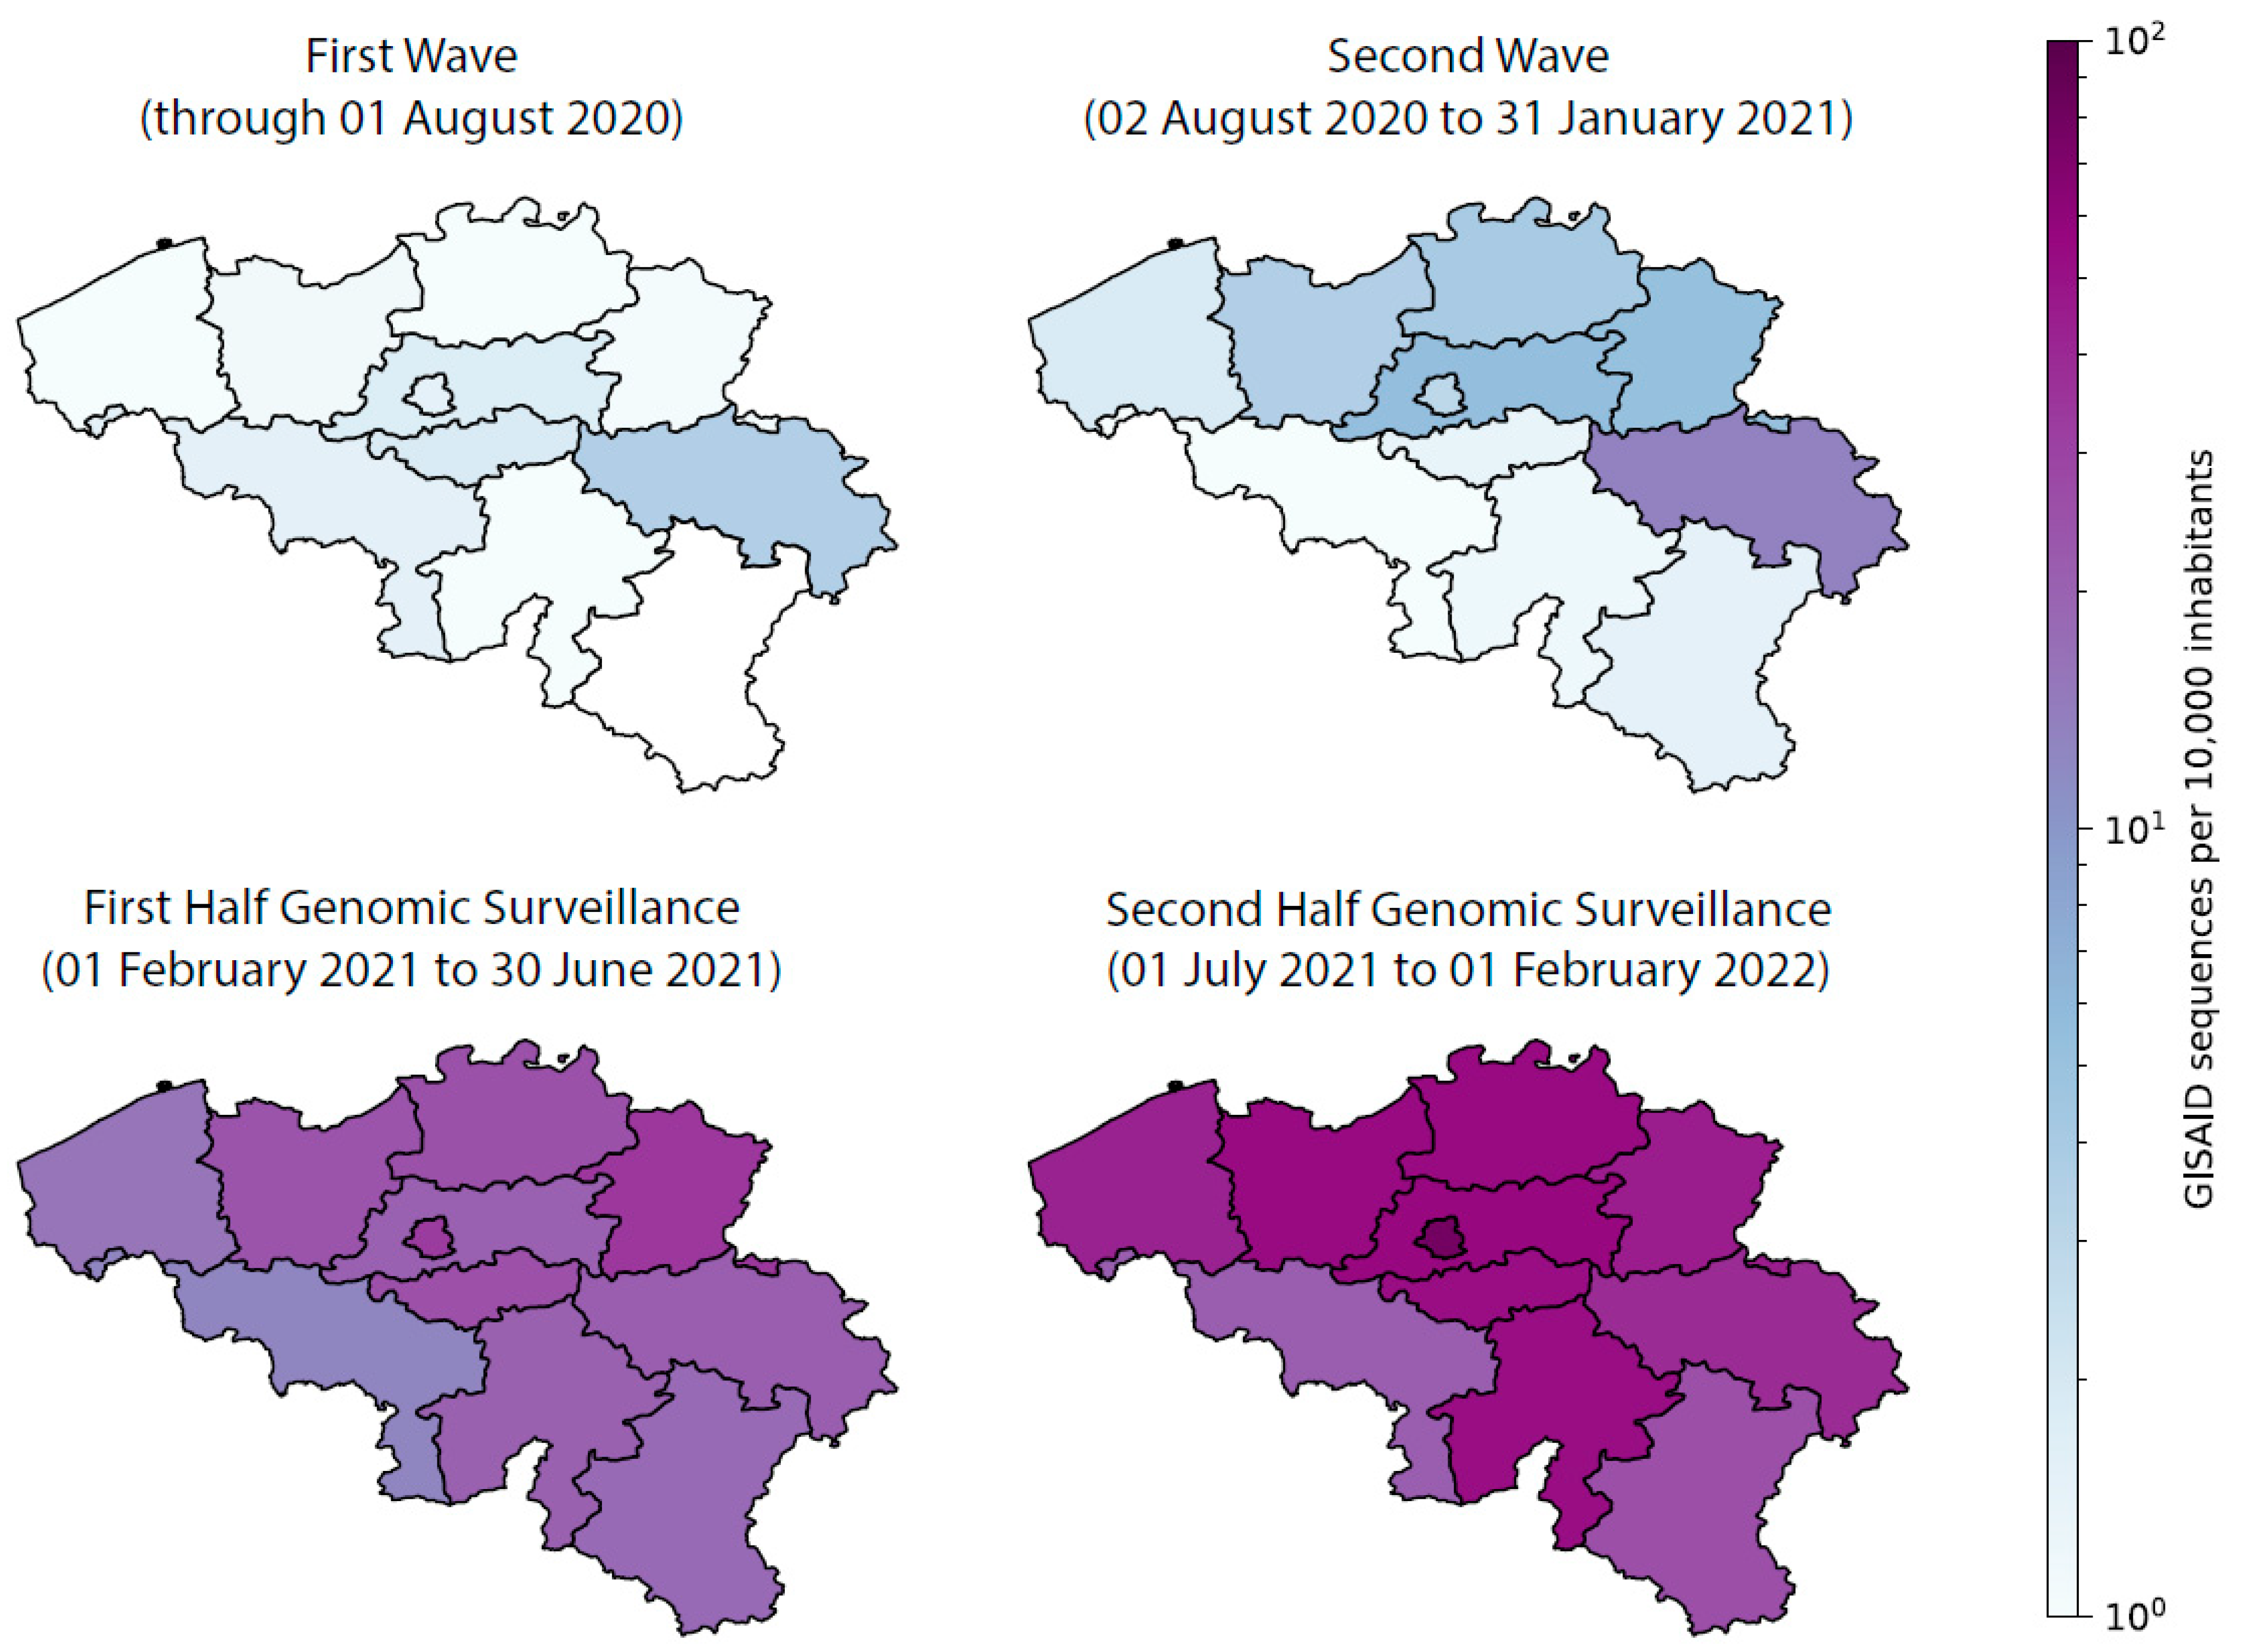
\includegraphics[width=.7\textwidth]{fig1}
  \caption[Total SARS-CoV-2 genomes in Belgium]{Number of available \gls{sarscov2} genomes for Belgium---per 10,000 inhabitants---on the public GISAID database since the start of the COVID-19 pandemic.}
  \label{fig:beGenomesPer10k}
\end{figure}

As part of the NRC for Respiratory Pathogens, UZ/KU Leuven was the first laboratory in Belgium to diagnose COVID-19 cases by \gls{pcr}, identifying the first Belgian case on 3 February 2020.
From the start and throughout the first year of the pandemic, a geographically heterogeneous share of the samples collected on a national level (Fig.~\ref{fig:beGenomesPer10k}) was analyzed in the clinical laboratory of UZ Leuven, providing a unique opportunity for a national genomic surveillance initiative.
Although without structural funding at that time, over 750 complete \gls{sarscov2} genomes of samples originating from the first epidemiological wave (March to June 2020) in Belgium were sequenced to characterize the temporal and geographic distribution of the COVID-19 pandemic in Belgium through phylogenetic and variant analysis.
\citet{wawina-bokalanga2021genetic} showed the presence of the major \gls{sarscov2} clades (G, GH and GR) and lineages circulating in Belgium at that time.
The continuation of this initiative to sequence a share of the positive samples, conducted by the different sequencing centers at that time, resulted in a total of over 3700 genomes in Belgium by the end of 2020.

In order to inform authorities, the scientific community, and the general public on the evolution and spread of \gls{sarscov2} in Belgium, we used the available genomes to construct our first Belgian Nextstrain instance, which became publicly available on 8 January 2021 (see Fig.~\ref{fig:beFirstMap}).
Nextstrain's joint temporal and spatial visualizations integrate sequence data with geographic information, lineage nomenclature, and mutations of interest to show how the pandemic unfolded over time, delivering important insights to health professionals, epidemiologists, virologists, and the general public via easily shareable links (for example, through social media) \citep{hadfield2018nextstrain}.

% Figure 2
\begin{figure}[ht]
  \centering
  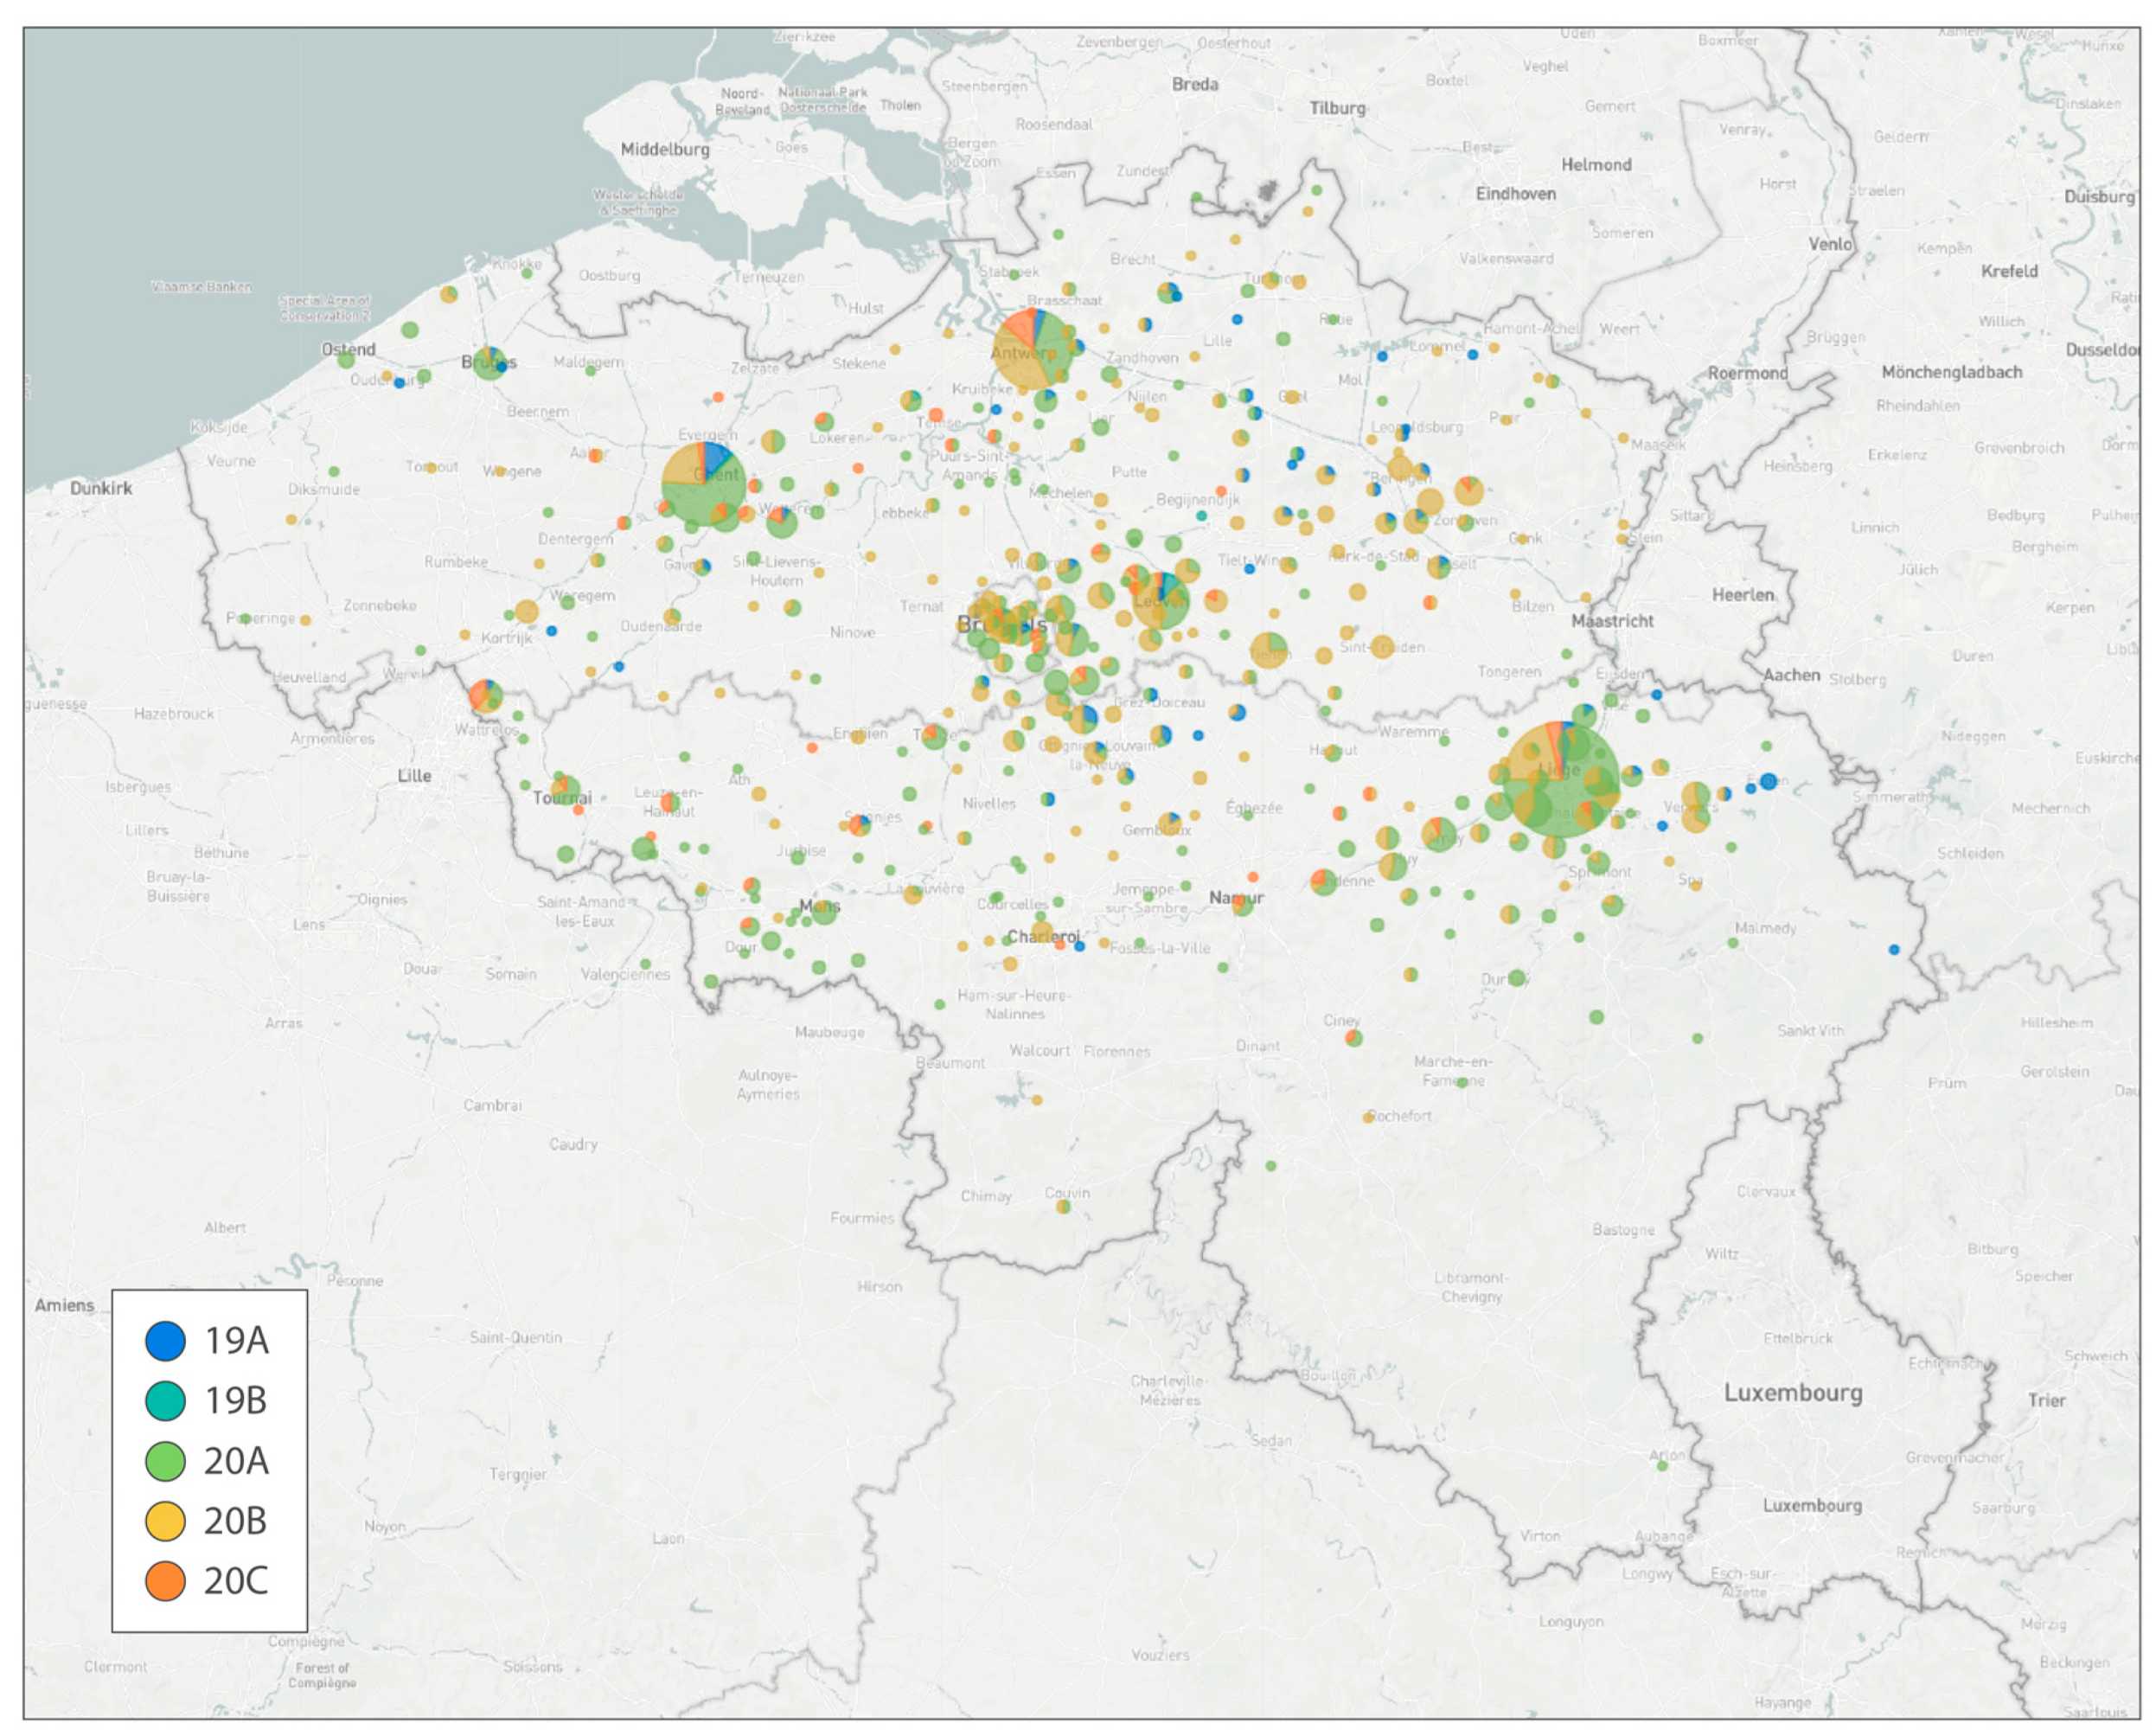
\includegraphics[width=.7\textwidth]{fig2}
  \caption[First Belgian Nextstrain map]{First publicly available Nextstrain build for Belgium, released on 8 January 2021 (just before the Alpha variant was detected in Belgium—or at least before any genomes from Alpha were available). In cases where GDPR prevents sharing the patient's actual municipality of residence the sequencing center's location was used, leading to larger numbers for the cities of Leuven, Li\`{e}ge, Ghent, and Antwerp. Pie charts are colored according to the \gls{sarscov2} clades defined in Nextstrain.}
  \label{fig:beFirstMap}
\end{figure} 

Further, the availability of such a large collection of genomes resulted in various \gls{sarscov2} studies to which members of the genomic surveillance network were able to contribute, before a national initiative was even set up.
These studies primarily focused on the evolution and spread of \gls{sarscov2} in Belgium and Europe \citep{alm2020geographical}.
\citet{dellicour2021phylodynamic} developed a phylodynamic workflow that combines maximum-likelihood phylogenetic inference with Bayesian phylogeographic inference to rapidly analyze the spatiotemporal dispersal history and dynamics of \gls{sarscov2} lineages.
At the time of their analysis (10 June 2020), Belgium had one of the highest spatial densities of available \gls{sarscov2} genomes—with 740 genomes sequenced, owing to the aforementioned research initiatives—which allowed \citet{dellicour2021phylodynamic} to apply their method on the pandemic situation in Belgium and identify a large number of lineage introductions into the country.
Making use of this workflow and focusing on the second European pandemic wave (March--November 2020), \citet{bollen2021exploiting} further employed Bayesian phylogeographic inference on each clade occurring in the province of Li\`{e}ge.
The authors focused on inferring the regional dispersal history of viral lineages associated with three specific mutations on the spike protein (S98F, A222V and S477N) and quantifying their relative importance through time.

Several studies focused on very specific settings to study \gls{sarscov2} infections among Belgian residents.
At the beginning of May 2020, 22 out of 70 Belgian soldiers deployed to a military education and training center in Maradi, Niger, developed mild COVID-19 compatible symptoms \citep{pirnay2020study}.
Immediately upon their return to Belgium, and two weeks later, all seventy soldiers were tested for \gls{sarscov2} RNA and antibodies.
Nine soldiers had at least one positive COVID-19 diagnostic test result.
Five of them exhibited COVID-19 symptoms (mainly anosmia, ageusia, and fever), while four were asymptomatic.
Conventional and genomic epidemiological data suggested that these infections had a most recent common ancestor with African origin and that the Belgian military service men were infected through contact with locals.

Using postmortem COVID-19 cases to perform detailed virological analysis could provide proof of viremia and presence of replication-competent \gls{sarscov2} in extrapulmonary organs of immunocompromised patients, including heart, kidney, liver and spleen \citep{vancleemput2021organ-specific}.
In parallel, organ-specific \gls{sarscov2} genomic diversity and mutations of concern have been identified prior to the emergence of \gls{voc}s.
Based on disease duration and viral loads in plasma and lungs, two stages of fatal disease evolution were addressed by Van Cleemput et al., providing insights about the pathogenesis and intra-host evolution of \gls{sarscov2} in immunocompromised patients.

Nursing homes constitute a highly vulnerable setting for the introduction and spread of \gls{sarscov2} among their inhabitants, staff, and visitors.
\citet{vuylsteke2022role} describes a massive outbreak of COVID-19 after a cultural event in a nursing home in Flanders, Belgium, at the end of 2020.
Within days of the event, nursing home residents started to display symptoms, and the outbreak spread rapidly within the nursing home, leading to a total of 127 residents and 40 staff members being diagnosed with \gls{sarscov2} since the beginning of the outbreak.
\citet{vuylsteke2022role} claim that airborne transmission was the most plausible explanation for the massive intra-facility spread, which underscores the importance of ventilation and air quality for the prevention of future outbreaks in such closed facilities.

Some of the earliest \gls{sarscov2} genomes sequenced in Belgium at the start of the pandemic were used to develop a novel Bayesian phylogeographic inference methodology that is able to exploit the individual travel histories of infected patients.
\citet{lemey2020accommodating} show that making use of such travel history data yields more realistic hypotheses of virus spread, and can suggest alternative routes of virus migration that are plausible within the epidemiological context but are not apparent when sampling efforts are limited or highly heterogeneous in the affected countries.

Following this study, \citet{lemey2021untangling} built a phylogeographical model to evaluate how newly introduced lineages, as opposed to the rekindling of persistent lineages, contributed to the resurgence of COVID-19 in Europe in late summer, 2020.
The authors informed their model using genomic, mobility, and epidemiological data from 10 European countries and estimated that in many countries, more than half of the lineages circulating in the late summer of 2020 resulted from new introductions, and that the success in onward transmission of newly introduced lineages was negatively associated with the local incidence of COVID-19 during this period.


\subsection{Setting Up the National Genomic Surveillance Platform for SARS-CoV-2 in Belgium}
In late 2020, as a response to the need to implement a more efficient genome surveillance program in Belgium, due to increasing concerns about the Alpha, Beta and Gamma \gls{voc}s, a coordinated sequencing and surveillance strategy was set up by the NRC UZ/KU Leuven in collaboration with the national public health institute, Sciensano.
Rapidly, a large national sequencing consortium combined forces to substantially scale up the national sequencing capacity in the early months of 2021.
This coordinated strategy focused on nationwide genomic sequencing in order to detect transmission hotspots and the possible (re-)emergence of recent variants first detected in the UK and South Africa, or any other variants for that matter.
Enhanced molecular surveillance was aimed at monitoring \gls{sarscov2} diversity more closely in space and time across the country.
Specifically, this initiative enabled the tracking of \gls{voc} frequency, as well as their circulation within the country.
Furthermore, it provided an early warning system in the case of the emergence of potentially more transmissible, virulent, or vaccine-escaping strains.
We note that while the official start of the nationwide genomic surveillance initiative was at the end of February 2021, many labs had already started their sequencing efforts at the beginning of the year, thereby strengthening surveillance in anticipation of the nationwide initiative.
This can be seen in Fig.~\ref{fig:beGenomesPer10k}, which shows a strong increase in available genome sequences across all Belgian provinces since the start of the national \gls{sarscov2} genomic surveillance initiative.

At the inter-ministerial conference for public health on 20 January 2021, it was decided that special attention should be given to the proactive detection and monitoring of circulating variants of the \gls{sarscov2} virus.
A conceptual note was presented at the insurance committee on 22 February 2021, followed by the drafting of a detailed two-pillar model of surveillance efforts: a national genomic surveillance consortium, fueled by a sentinel laboratory network for the supply of a representative share of their positive samples.
In mid-March, a call was launched to all laboratories in Belgium to apply to be part of the national genomic surveillance consortium for \gls{sarscov2}, coordinated by the NRC UZ/KU Leuven with the support of Sciensano.
Following this candidacy call, a network of 17 laboratory network partners was initiated to be responsible for the \gls{sarscov2} genomic surveillance in Belgium, of which the majority of centers signed a convention for reimbursement purposes (Fig.~\ref{fig:bePipeline}).
To this end, based on a predefined required sequencing capacity per Belgian province (based on the number of inhabitants rather than infections, as the latter would fluctuate over time), a minimum of 1150 genome sequences needed to be generated per week, roughly aiming to sequence at least 5\% of all positive cases diagnosed within Belgium.

% Figure 3
\begin{figure}[ht]
  \centering
  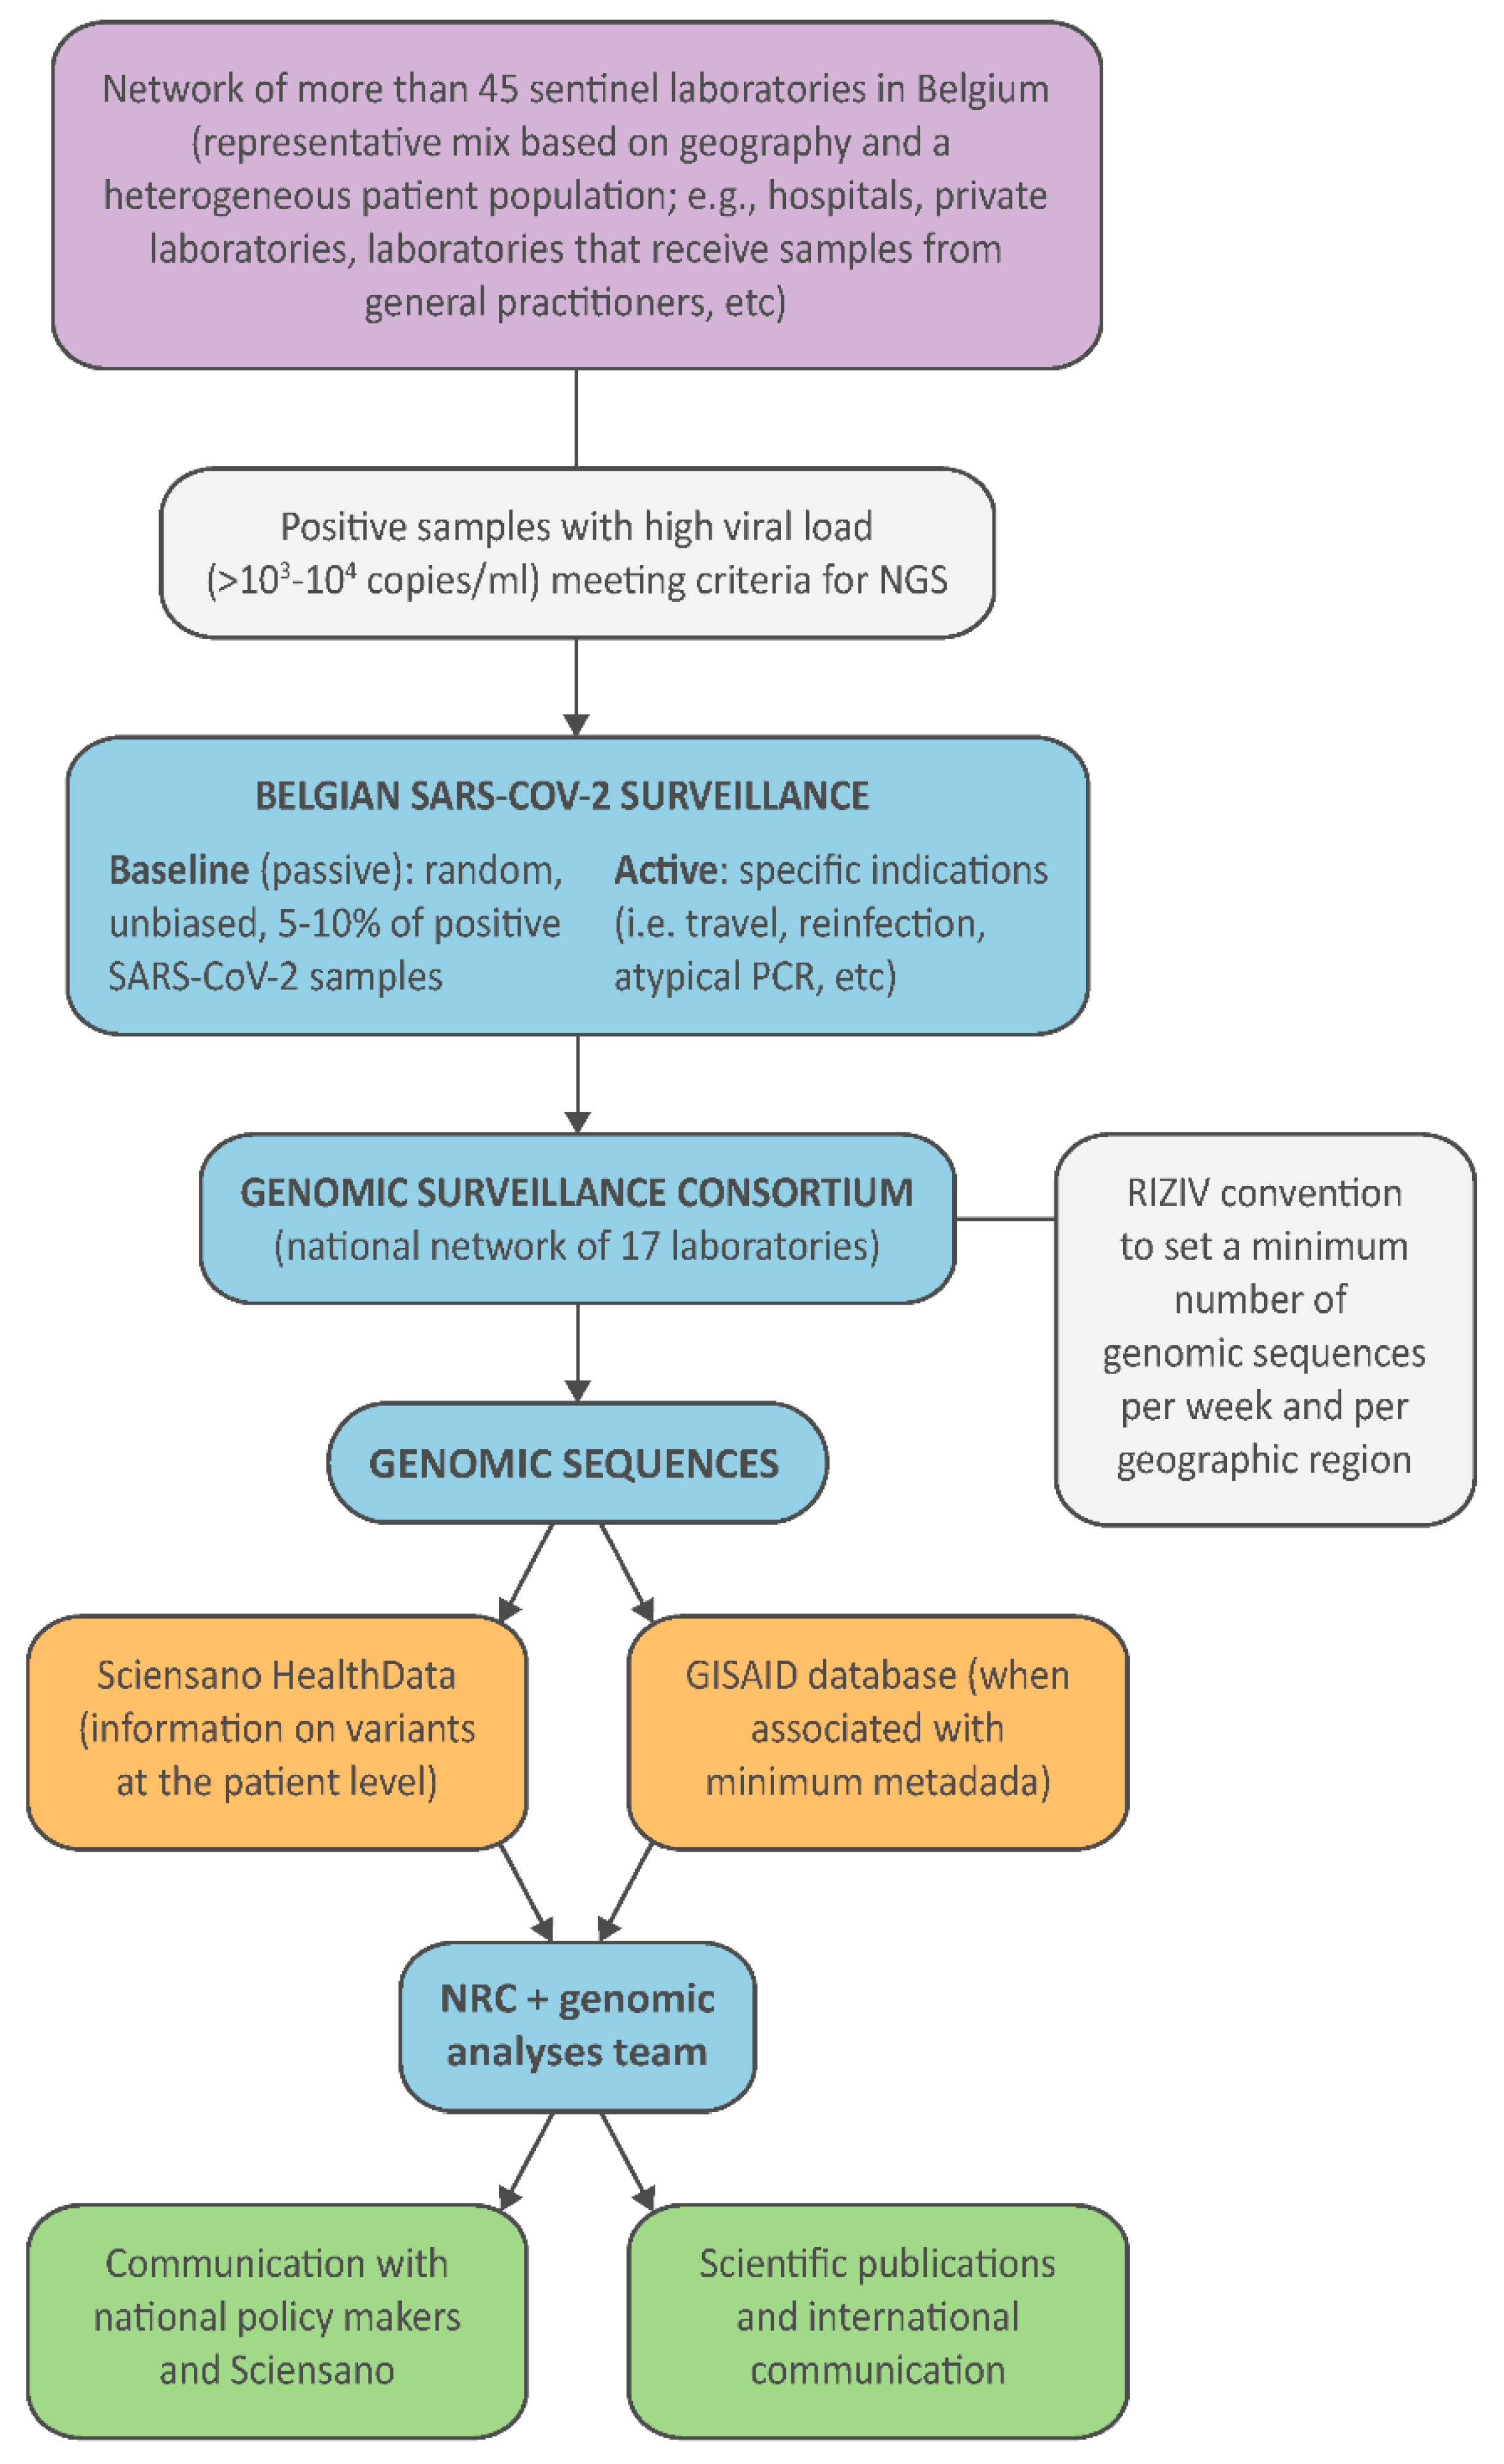
\includegraphics[width=.6\textwidth]{fig3}
  \caption[Genomic surveillance pipeline]{Workflow of the \gls{sarscov2} genomic surveillance established in Belgium. ``NRC'' stands for National Reference Center (and in this context refers to the NRC for respiratory pathogens), ``RIZIV'' for National Institute for Health and Disability, and ``NGS'' for next-generation sequencing.}
  \label{fig:bePipeline}
\end{figure} 

The year following the start of the nationwide genomic surveillance initiative in Belgium saw an important increase in the sequencing coverage of positive cases, rising from 1\% to nearly 4\% (Fig.~\ref{fig:euGenomeCounts}).
While the initial sequencing coverage of positive cases of 1\% already put Belgium at a recently proposed threshold/benchmark for rapidly detecting circulating \gls{sarscov2} variants through random sampling, this increase put Belgium closer towards ensuring the rapid detection of viral lineages, according to a recent simulation study \citep{brito2022global}.
This increase puts Belgium just below several other European countries in terms of coverage of positive cases, including Germany, Austria, Norway, and Finland, but ahead of the Netherlands, France, Portugal, and Spain.
Of note, this sequencing coverage of positive cases has been highly variable throughout the pandemic, directly related to the number of cases associated with the different pandemic waves of infections.
During times when there has been a relatively low number of infections, sequencing coverage of positive cases was shown to reach nearly 25\% of cases (Fig.~\ref{fig:beSeqCoverage} and Fig.~\ref{fig:beCasesSciensano}), whereas during epidemic peaks of infections, the imposed threshold of 5\% could not be reached consistently.

% Figure 4
\begin{figure}[ht]
  \centering
  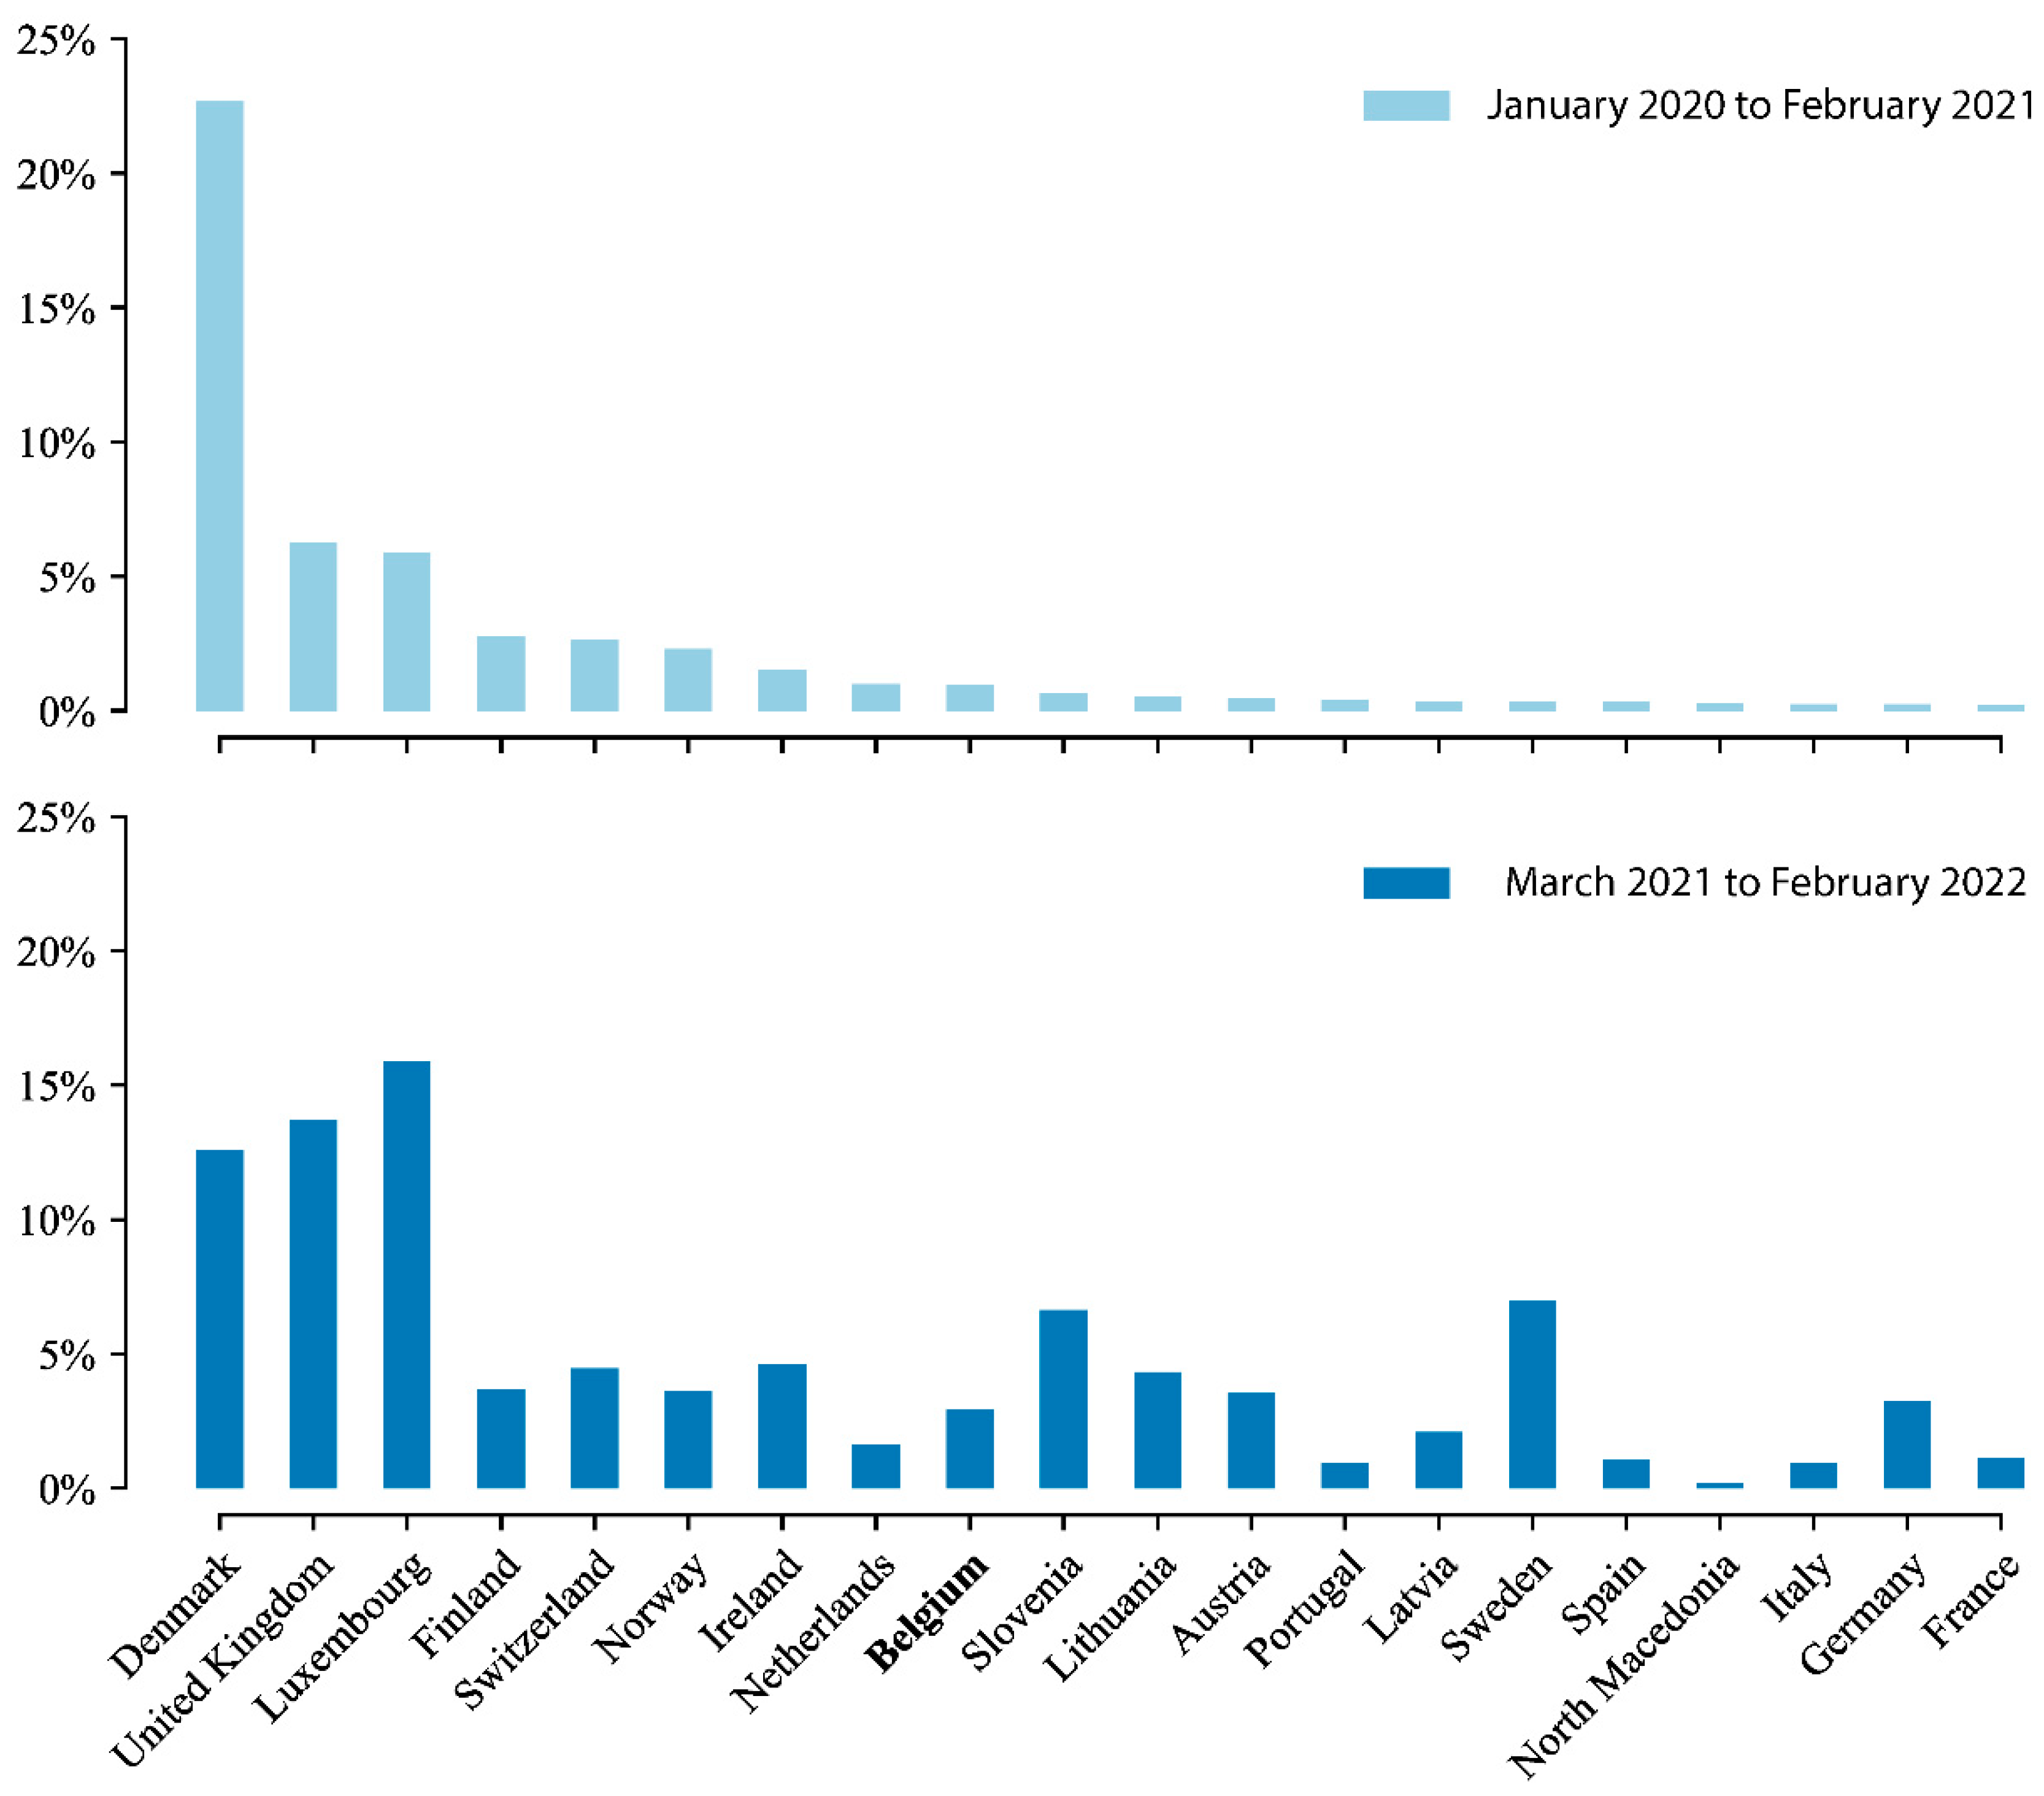
\includegraphics[width=.8\textwidth]{fig4}
  \caption[European sequencing coverage 2020--2022]{Sequencing efforts for European countries that reported over 10,000 positive cases on a given year, expressed as the percentage of confirmed COVID-19 cases sequenced that have been submitted to GISAID (retrieved from the GISAID database on 31 August 2022), with a minimum sequence/case ratio of 0.1\%. Top: Sequencing coverage of positive cases prior to the establishment of the COVID-19 Genomics Belgian Consortium, from January 2020 to the end of February 2021. Bottom: Sequencing coverage of positive cases a year after the establishment of the consortium, from 1 March 2021 to the end of February 2022. Large discrepancies can be seen among European countries, both before and after March 2021, with Belgium's performance in 2021 at a similar level as most of its neighboring countries.}
  \label{fig:euGenomeCounts}
\end{figure}

% Figure 5
\begin{figure}[ht]
  \centering
  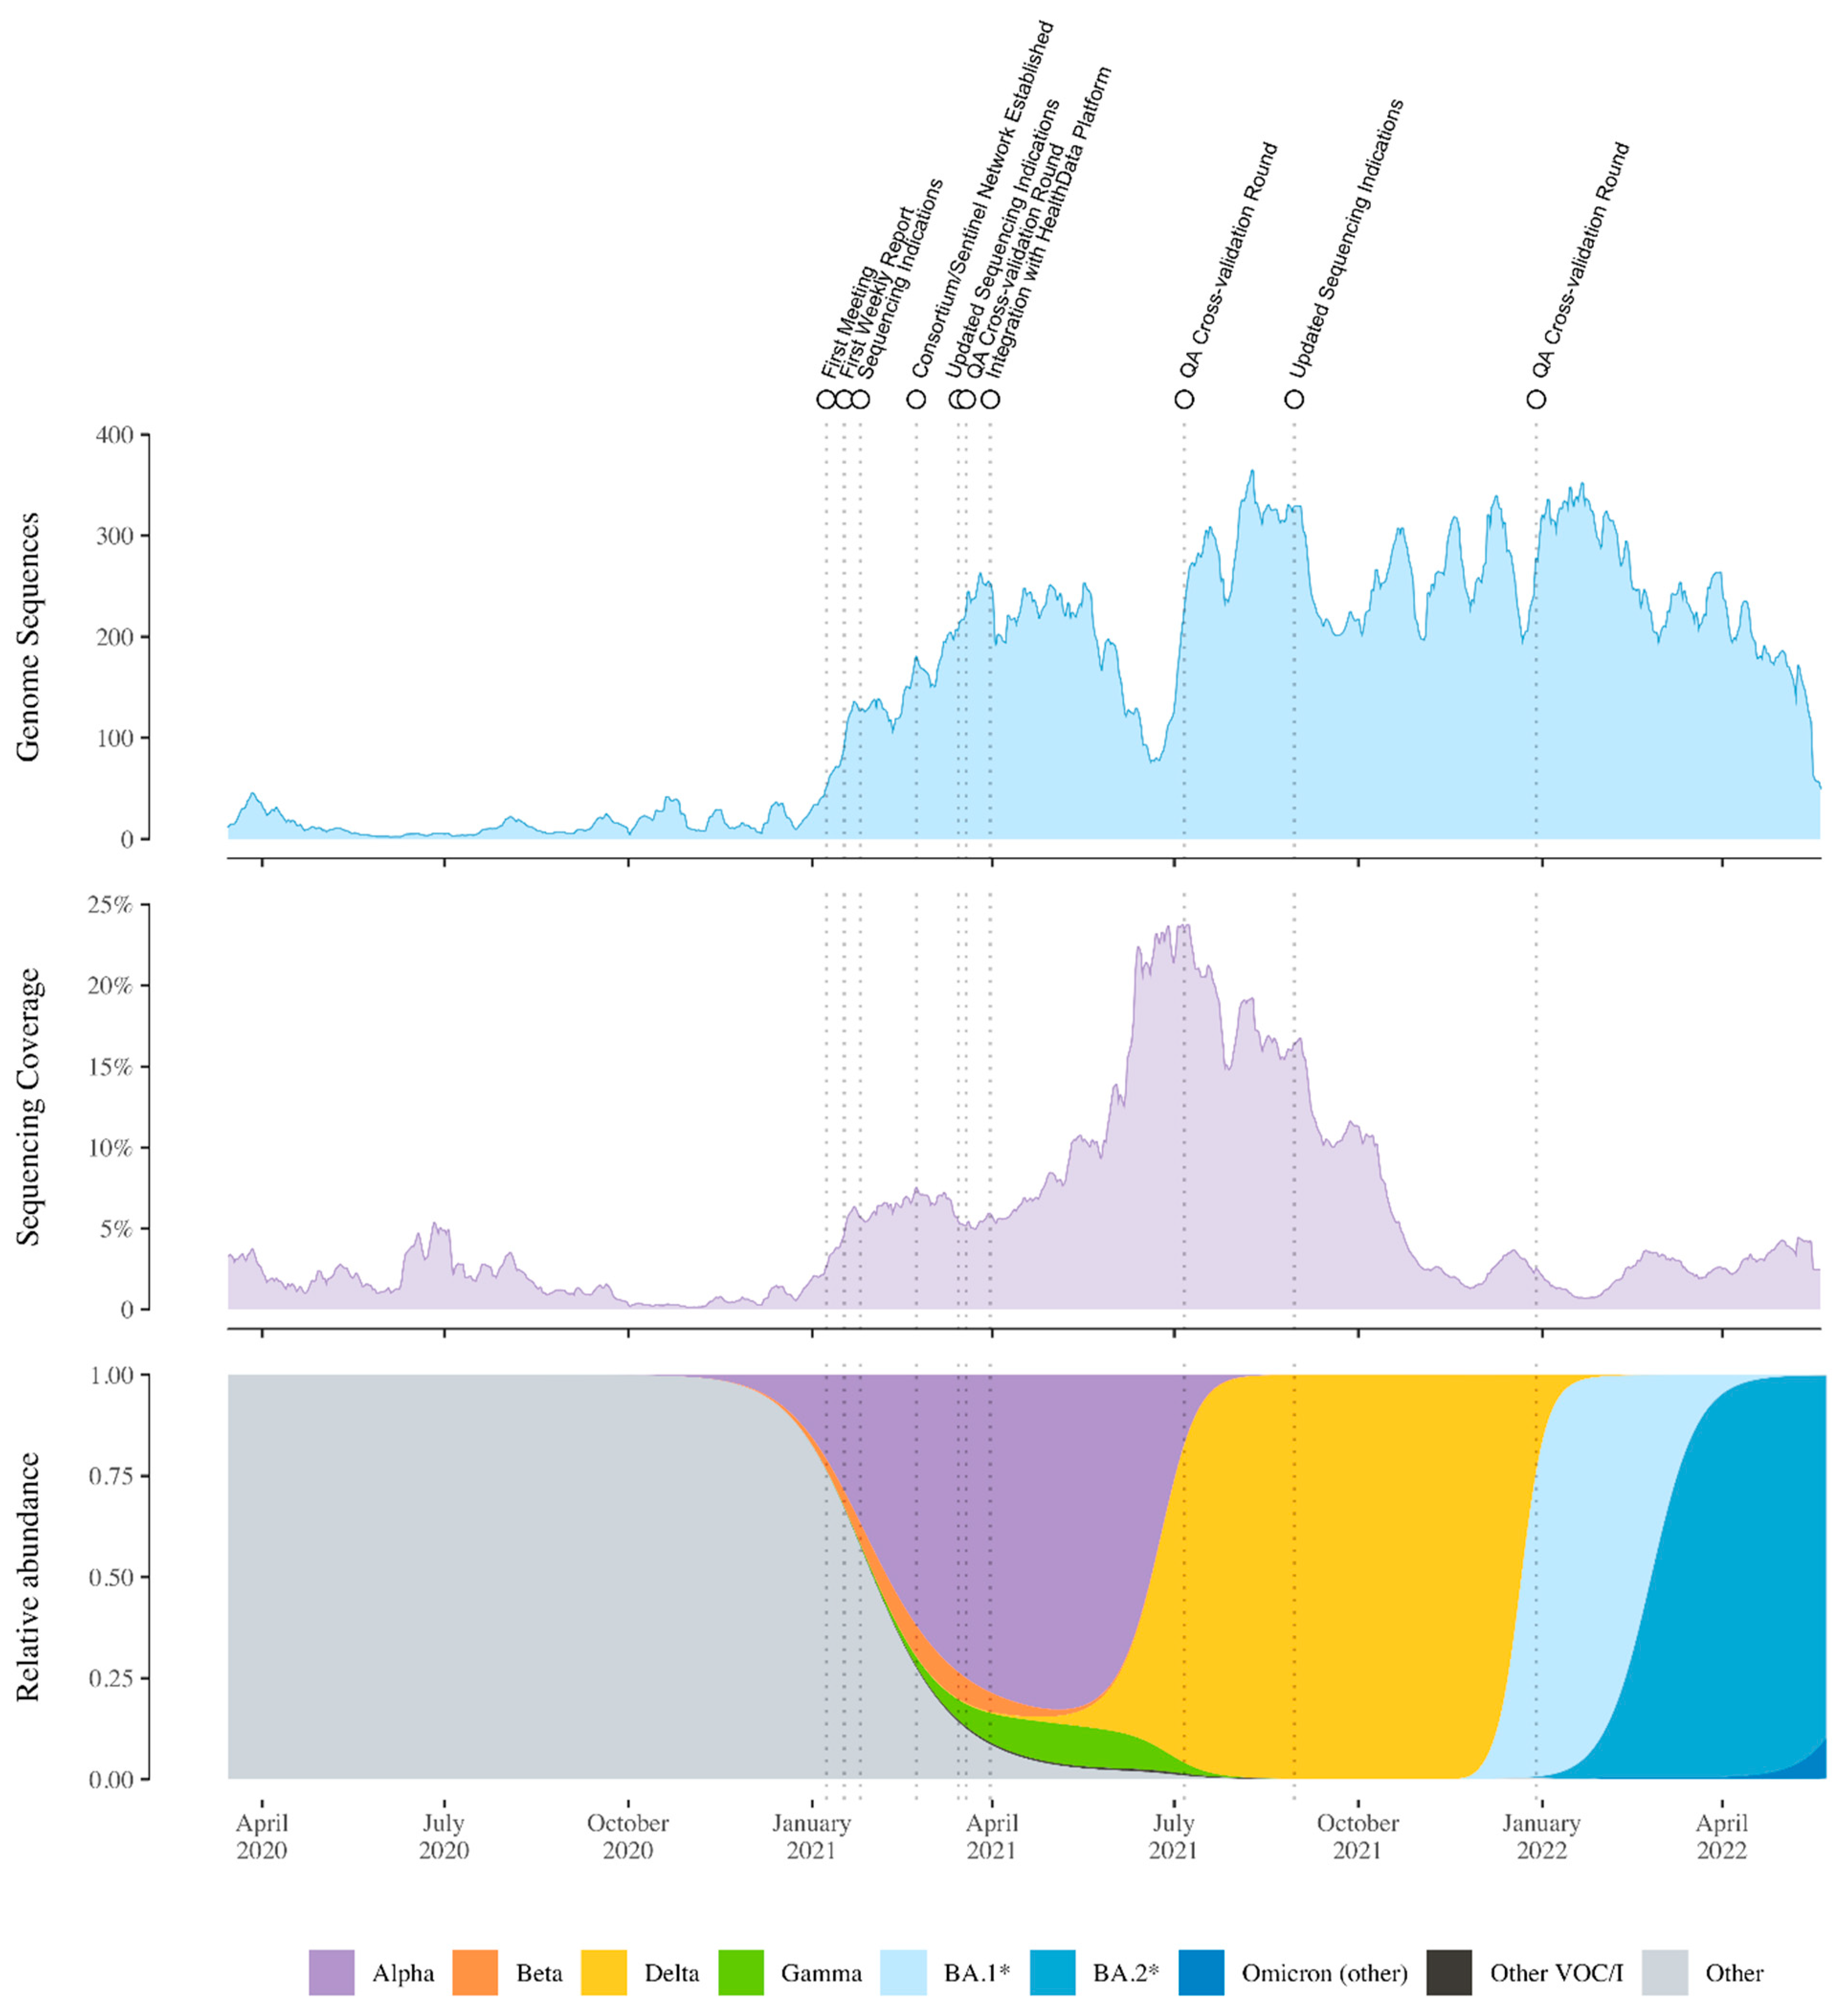
\includegraphics[width=.95\textwidth]{fig5}
  \caption[Belgian sequencing coverage]{Sequencing numbers, sequencing coverage (the ratio between genomes sequenced and confirmed cases), and relative abundance of \gls{sarscov2} variants of concern in Belgium.
  Individual colors were assigned to lineages depending on their \gls{voc} status and prevalence in Belgium.
  Dotted lines indicate events related to the COVID-19 Belgium Genomics Consortium.}
  \label{fig:beSeqCoverage}
\end{figure}

% Figure 6
\begin{figure}[!ht]
  \centering
  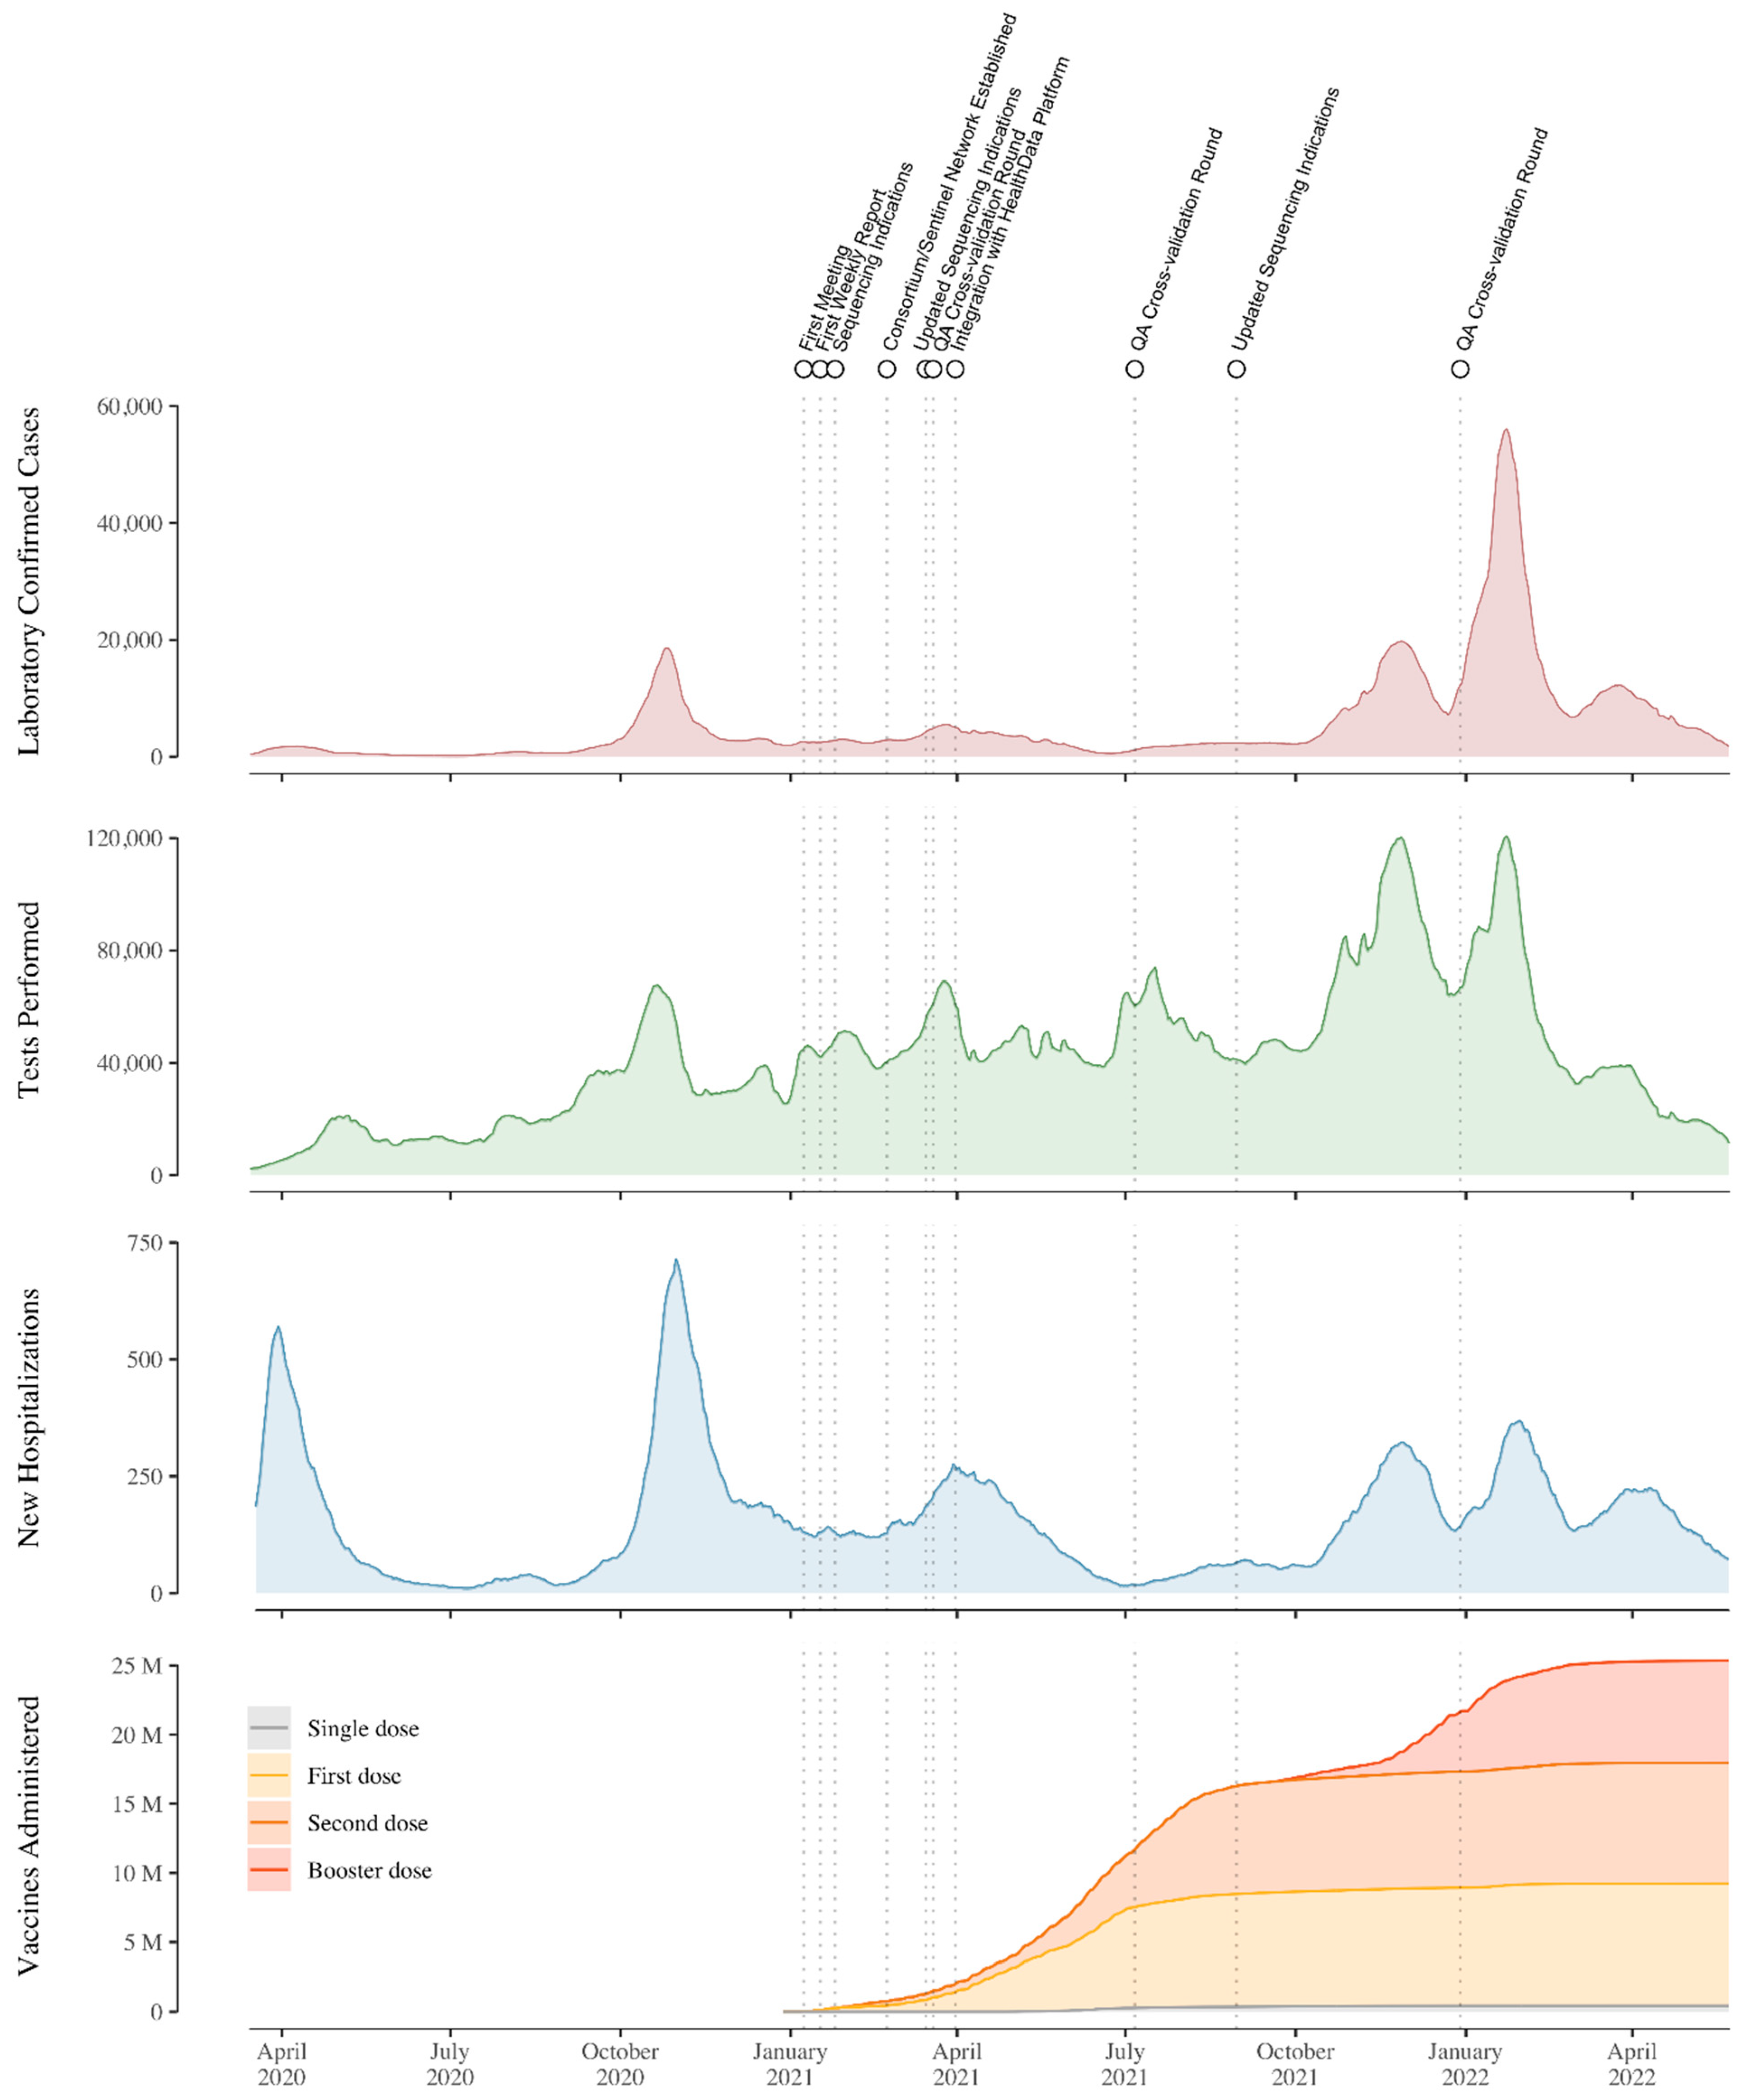
\includegraphics[width=.9\textwidth]{fig6}
  \caption[Confirmed cases, tests, hospitalizations, \& vaccinations]{Daily number of confirmed cases (7-day moving average), daily number of COVID-19 tests performed (7-day moving average), new hospitalizations (new daily admissions to hospital of lab-confirmed COVID-19 patients, with a 7-day moving average) and cumulative number of vaccines administered in Belgium from March 2020 to May 2022. Data retrieved from Sciensano, Belgium's national public health institute (\url{https://epistat.sciensano.be/covid} (accessed on 22 August 2022)). Dotted lines indicate events related to the COVID-19 Belgium Genomics Consortium. Peaks in cases and hospitalizations roughly align with moments where the different \gls{voc}s were dominant.}
  \label{fig:beCasesSciensano}
\end{figure}

In Europe, Iceland, the UK, and Denmark have been particularly credited for their massive genomic sequencing efforts throughout the pandemic (Fig.~\ref{fig:euGenomeCounts}), with Denmark deciding to sequence every positive case during certain periods throughout the pandemic, and Iceland sequencing up to 90\% of positive cases during the first year of the pandemic.
In the UK, the COVID-19 Genomics UK Consortium (COG-UK), established in April 2020, undertook sequencing of \gls{sarscov2} samples from a target of 10\% of confirmed positive cases, which translated to an average of 6800 sequences per week during its first year (\verb|www.cogconsortium.uk| (accessed on 22 June 2021)).
For comparison, during the same time period, Denmark averaged approximately 1000 sequences per week and the Netherlands averaged 370 sequences per week.
Prior to the establishment of the Belgian consortium, in terms of sequencing efforts within Europe, Iceland and Denmark attained higher numbers than the UK, with a coverage of 71\% and 23\% of confirmed positive cases, respectively.
Meanwhile, Luxemburg sequenced approximately 6\%, Finland, Norway and Switzerland roughly 2\%, and Ireland, Belgium and the Netherlands nearly 1\% (Fig.~\ref{fig:euGenomeCounts}).

The two-pillar model of genomic surveillance consists of, on the one hand, an unbiased and random sequencing of cases, called baseline (or passive) surveillance, while on the other hand, the pillar of active surveillance focused on specific questions, populations, or settings, as determined through official sequencing indications proposed by the risk-assessment group (RAG).
In the context of baseline surveillance, samples are collected through a country-wide network of almost 50 sentinel \gls{pcr} laboratories (Fig.~\ref{fig:bePipeline}), geographically dispersed across Belgium and selected to be representative of the heterogeneous population of persons being infected with \gls{sarscov2} (including hospital and private laboratories as well as federal testing platforms).
The selection of these participating laboratories ensured a wide community-based sequencing coverage of positive cases in all Belgian provinces (Fig.~\ref{fig:beFirstMap}), while in the context of active surveillance, samples could be sent to the sequencing laboratories from all diagnostic COVID-19 testing laboratories across Belgium, including testing laboratories of the main airports in Belgium (located in Zaventem and Charleroi) to monitor import events.
Apart from returning travelers, active surveillance was initially focused on reinfection cases, post-vaccination breakthrough samples, atypical \gls{pcr} results (e.g., dropout or shift in viral load for one of the target genes of a \gls{pcr} assay), outbreak settings, and populations at risk for mutations (e.g., immunocompromised patients \citep{vandermoeren2022viral}).
Throughout the pandemic, there was a specific request to obtain and sequence samples in large outbreak settings, such as elderly care facilities (e.g., \citep{vuylsteke2022role}), hospitals, or schools, to identify potential superspreaders and fine-tune biosecurity measures.
Evolving towards a higher vaccination coverage (see Fig.~\ref{fig:beCasesSciensano}), post-vaccination breakthrough cases were asked to be sequenced only in particular situations, such as residents of long-term care facilities or when associated with increased disease severity.
Along the road, it was requested that sequencing efforts be reinforced for the hospitalized population, mapping in detail the circulation of variants within hospitals and particular units in detail, allowing for association studies between different \gls{voc}s and disease severity (\citep{vangoethem2022severity,vangoethem2022clinical}, but see also Section~\ref{ssec:beGenSurPapers}).

As among the national sequencing network, various sequencing protocols and bioinformatics pipelines were implemented to detect and monitor the circulation of \gls{sarscov2} variants, and no official or commercial external quality control assessment was in place for \gls{sarscov2} WGS at the start of the genomic surveillance consortium, quality assurance was decided to be the responsibility of the coordinator of the consortium, i.e., the NRC UZ/KU Leuven, supported by Sciensano.
Overall, eight laboratory networks implemented a sequencing protocol relying on Illumina sequencing technology, while nine centers obtained \gls{sarscov2} full-length sequences using the Oxford Nanopore Technology.
In the first year of the national genomic surveillance initiative, three cross-validation rounds were organized (see also Fig.~\ref{fig:beSeqCoverage} and Fig.~\ref{fig:beCasesSciensano}), in which all sequencing laboratories with a signed convention in a context of reimbursement were required to participate.
All sequencing centers were asked to supply the NRC with three to five samples of sufficient leftover material after initial sequencing at their facility, corresponding to different \gls{sarscov2} variants.
Sequencing information of the initial sequencing center was also shared with the NRC to facilitate the evaluation of the cross-validation round.
At the level of the NRC, new panels were constructed and sent out to the participating sequencing laboratories, consisting of a mix of \gls{sarscov2} variants, different transport media, and with each sample being ideally sent to at least two laboratories (that make use of different sequencing technologies) to render a broad comparison of results possible.
The participating laboratories were asked to analyze the received panel according to their standard operating procedures and to report the results within a turnaround of seven working days (as agreed upon in the convention) to the NRC.
A thorough evaluation of the results occurred at the level of the NRC, and a report with action points (when appropriate) was shared with all the participating laboratories.
Apart from quality assurance, monthly meetings were organized with all members of the sequencing consortium by the NRC UZ/KU Leuven to discuss the setup of the surveillance and associated sequencing coverage of positive cases, data reporting, joint projects, and publications, as well as active troubleshooting.
To facilitate joint projects and publications within the large group of partners within the consortium, ethical approval was obtained by the NRC UZ/KU Leuven as coordinating center and with all other centers as co-investigators (S66037).
To inform a broad audience, and especially policymakers, of the detailed and near real-time circulation of \gls{sarscov2} variants in Belgium, weekly reports were written and published on the website of the Department of Laboratory Medicine, UZ Leuven, starting 17 January 2021, and these are ongoing today (\url{https://www.uzleuven.be/nl/laboratoriumgeneeskunde/genomic-surveillance-sars-cov-2-belgium} (accessed on 19 October 2022)).
At the time of writing, 102 reports have been written and disseminated.

The sequencing centers that received samples were responsible for reporting the results to the respective laboratories or prescribing clinicians that requested the sequencing analysis, as well as reporting in real-time the variant information to Sciensano, through the national data platform called healthdata.be, using the message `LaboratoryTestResultVariants', through which variant information obtained by both presumptive genotyping (such as the use of marker \gls{pcr}s) and WGS could be transferred (\url{https://docs.healthdata.be/nl/node/286} (accessed on 8 June 2022)).
This dataflow provided for, amongst others, the weekly reporting in the epidemiological bulletin of Sciensano, the real-time reporting on the public dashboard of Sciensano, and reporting to the \gls{ecdc}.
Furthermore, as stated in the convention, the sequencing centers were also responsible for making the actual nucleotide sequences, annotated with minimal metadata (e.g., age, gender, location, and sequencing indication), publicly available through submission to the international database GISAID \citep{shu2017gisaid}.
These sequences were used to update both global and Belgium-focused Nextstrain builds (e.g., Fig.~\ref{fig:beFirstMap}) and to transparently inform public health authorities on the circulation of the different variants of the virus (e.g., results of these analyses are often used in the weekly reports of the consortium).
The combination of an extensive spatial sequencing coverage and the integration of a sufficiently representative number of positive samples allowed for the minimization of noise inevitably generated by project-centered sequencing initiatives leading to the over-representation of some regions (see Fig.~\ref{fig:beGenomesPer10k}) or particular patient groups.


\subsection{Studies Resulting from the Genomic Surveillance Initiative}\label{ssec:beGenSurPapers}
As mentioned in the previous section, the genomic sequences generated by the consortium enabled collaboration on many joint publications, which we discuss here in chronological order (of the variants being studied).

\citet{vangoethem2022severity} compared COVID-19 disease severity between hospitalized patients in Belgium infected with the \gls{sarscov2} variant B.1.1.7 (Alpha) and those infected with previously circulating strains.
Employing a causal framework, the authors observed no difference between patients infected with B.1.1.7 and those infected with older strains in terms of disease severity or in-hospital mortality.
However, \citet{vangoethem2022severity} found that the estimated standardized risk of being admitted to an ICU was significantly higher when infected with the B.1.1.7 variant, and that among the younger age group ($\leq$65 years), B.1.1.7 was significantly associated with both severe COVID-19 progression and ICU admission.

Belgian Armed Forces that engaged in missions and operations around the world were systematically screened, pre- and post-mission, for the presence of \gls{sarscov2}, including the identification of viral lineages.
A study by \citet{pirnay2021variant} showed that nine distinct viral genotypes were identified in soldiers returning from operations in Niger, Congo, Afghanistan, and Mali.
The \gls{sarscov2} lineages identified included the variant of interest (\gls{voi}) B.1.525, the variant under monitoring (VUM) A.27, as well as lineages B.1.214, B.1, B.1.1.254, and A.
Through contact tracing and phylogenetic analysis, \citet{pirnay2021variant} showed that the isolation and testing policies implemented by the Belgian military command appear to have been successful in containing the influx and transmission of these distinct \gls{sarscov2} variants into both military and civilian populations.
In a follow-up study dedicated to the A.27 \gls{sarscov2} lineage, \citet{kaleta2022antibody} performed Bayesian phylogeographic analyses obtained from national and international databases to reveal an origin of this lineage in Western Africa, and multiple introductions from there initiated a global spread of this lineage.
The authors performed neutralization assays to demonstrate an escape of A.27 from convalescent and vaccine-elicited, antibody-mediated immunity, and to show that the therapeutic monoclonal antibody Bamlanivimab, and partially the REGN-COV2 cocktail, fail to block infection by A.27.

At the start of the wave of infections spawned by the emergence of the \gls{sarscov2} Delta \gls{voc} (lineage B.1.617.2), \citet{vanelslande2022two} found two clusters of Delta infections in a group of 41 Indian nursing students who traveled from New Delhi, India, to Belgium via Paris, France.
Upon arrival in Belgium, the students were quarantined in eight different houses.
Four houses remained COVID-free during the 24 days of follow-up, while all 27 residents of the other four houses developed an infection during quarantine, including four residents who were fully vaccinated and two residents who were partially vaccinated.
Through phylogenetic analysis of the genomic sequences made available through the nationwide genomic surveillance, \citet{vanelslande2022two} could confirm that these quarantined house outbreaks were successfully contained and did not lead to secondary community transmission in Belgium.

\citet{cuypers2022comprehensive} studied the risk factors for fatal COVID-19 post vaccination in three large nursing home outbreaks (20--35\% fatal cases) by combining \gls{sarscov2} aerosol monitoring, whole-genome phylogenetic analysis, and immunovirological profiling.
Each outbreak was shown to have been likely caused by a single introduction event, though each time with a different variant (Delta, Gamma, and Mu).
Employing survival and time-to-event analysis, the authors found four factors as predictors of mortality: age, male sex, \gls{sarscov2} variant, and timing of infection.
Further, \citet{cuypers2022comprehensive} show that dementia or peak viral load were not predictive of fatal cases in the joint analysis of the three outbreaks but were significant predictors in single nursing homes.

As a result of intensifying genomic surveillance efforts in Belgium, \citet{vanmechelen2022identification} were able to identify the first infection within Europe with \gls{sarscov2} Omicron \gls{voc} (lineage B.1.1.529/BA.1), from a Belgian patient with a history of recent travel to Egypt.
This first detection of the Omicron \gls{voc} further enabled growing an isolate in cell culture to determine its sensitivity to nine monoclonal antibodies, as well as to antibodies present in 115 serum samples from COVID-19 vaccine recipients or individuals who have recovered from COVID-19 \citep{planas2022considerable}.
The authors found that Omicron was completely or partially resistant to neutralization by all monoclonal antibodies tested.
Further, they showed that sera from recipients of the BNT162b2 (Pfizer) or ChAdOx1 (AstraZeneca) vaccine, sampled five months after complete vaccination, barely inhibited Omicron, and that sera from COVID-19-convalescent patients collected 6 or 12 months after symptoms displayed low or no neutralizing activity against Omicron.
Similar low or absent neutralizing antibody activity was observed for BA.1 versus original lineage B (Wuhan-Hu-1) and Delta (B.1.617.2) in sera from individuals infected with \gls{sarscov2} prior to vaccination, from infection-na\"{i}ve individuals after three doses of BNT162b2 and from previously-infected individuals after three doses of BNT162b2 \citep{arin2022three}.
Subsequent early detection of the BA.2 lineage allowed \citet{bruel2022serum} to compare its sensitivity to neutralization by the aforementioned nine therapeutic monoclonal antibodies against that of BA.1.
The authors analyzed sera from 29 immunocompromised individuals up to one month after administration of the Ronapreve (casirivimab and imdevimab) and/or Evusheld (cilgavimab and tixagevimab) antibody cocktails.
\citet{bruel2022serum} showed that all treated individuals displayed elevated antibody levels in their sera, which efficiently neutralized the Delta \gls{voc}.
Sera from Ronapreve recipients did not neutralize lineage BA.1 and weakly inhibited lineage BA.2, whereas neutralization of BA.1 and BA.2 was detected in 19 and 29 out of 29 Evusheld recipients, respectively.

Starting in late 2020, Alpha was the first \gls{voc} to become dominant in Belgium, reaching a relative abundance of up to 82\%, whereas the Beta and Gamma \gls{voc}s only reached a maximum abundance of 7.7\% and 9.9\%, respectively.
The Belgian COVID-19 epidemic was then followed by waves where Delta, BA.1 (and descendants) and BA.2 (and descendants) were dominant.
The replacement of Delta with the Omicron \gls{voc} as the dominating lineage worldwide (Fig.~\ref{fig:beSeqCoverage}) resulted in possible co-infections of patients by different \gls{sarscov2} strains.
\citet{wawina-bokalanga2022genomic} report on such a co-identification of \gls{sarscov2} variants Omicron and Delta in two geographically unrelated cases.
Both patients reported no recent travel history abroad.
Such co-infection cases with different variants may lead to the emergence of novel \gls{sarscov2} recombinant variants, which might influence viral transmission, disease severity, and vaccine efficacy \citep{rehman2020evolutionary}.
Further, \citet{vangoethem2022clinical} assessed the risk for severe COVID-19, ICU admission, and in-hospital mortality in hospitalized patients when infected with the Omicron variant compared to when infected with the Delta variant.
Using data from 954 COVID-19 patients, of which 445 were infected with Omicron, the authors employed a causal framework to show that the estimated standardized risk for severe COVID-19 and ICU admission in hospitalized patients was significantly lower when infected with the Omicron variant, whereas in-hospital mortality was not significantly different according to the \gls{sarscov2} variant.


\subsection{Conclusions and Discussion}
We have here presented an overview through time of genomic surveillance efforts in Belgium, which evolved from non-structural, project-based initiatives to a nationwide approach following the establishment of a genomic surveillance consortium.
We have shown that initiating this consortium at the start of 2021 quickly resulted in a marked increase in the number of \gls{sarscov2} genomic sequences being generated in Belgium, as well as overall sequencing coverage of positive cases (Fig.~\ref{fig:beSeqCoverage}).
We have also provided an overview of the number of tests performed, alongside the number of cases detected, and the number of recorded hospitalizations, which are obviously all strongly correlated (Fig.~\ref{fig:beCasesSciensano}).
Of note, the Belgian Interministerial Public Health Conference asked the \gls{ecdc} to carry out an external evaluation of the testing policy applied by Belgium during June--December 2021, in response to the coronavirus disease 2019 (COVID-19) pandemic \citep{ecdcBelgiumTesting}.
As with the genomic surveillance, the \gls{ecdc} noted that testing strategies were first decided upon in Belgium by existing institutions, but during the crisis, other bodies were set up; testing strategies were developed based on scientific advice and have regularly been adapted, based on the epidemiological situation.
More importantly, and related to this review, the \gls{ecdc} found that Belgium performs comprehensive genomic surveillance and acknowledged that sequences were reported weekly, with volumes sufficient to estimate variant proportions of 2.5\% or lower, following \gls{ecdc} recommendations.

A similar benchmark was used recently in a pre-print to show that on average, genome surveillance programs in high income countries should be able to detect circulating virus lineages at 5\% prevalence with maximum probability under the assumption of random sampling, as shown by \citet{brito2022global} The authors have shown that when attaining a sequencing percentage of 5\% per week—the target imposed upon initializing the nationwide genomic surveillance in Belgium—there is a 48\% probability of detecting a viral lineage before it reaches 100 cases randomly selected from the population, provided a turnaround of 7 days can be achieved.
However, this probability can drop markedly with sequencing coverage of positive cases.
According to \citet{brito2022global}, when the proportion of sequenced cases per week decreases by 100-fold, to 0.05\%, the probability of the timely detection of a viral lineage before it reaches 100 cases decreases to 4.8\% for a turnaround of 7 days, and further declines to 2.6\% when turnaround time is 35 days.

Related to turnaround times for global data sharing, a retrospective analysis \citep{maher2022predicting} suggested that some of the key variant-defining mutations could potentially have been detected much earlier, which shows the importance of sharing data rapidly and globally, opening up the possibility of analyzing the data with a series of bioinformatics tools.
However, genomic data are not the sole source of information that contribute to the development and implementation of a global risk-monitoring framework for \gls{sarscov2} variants, as this requires a multidisciplinary approach that includes in silico, virological, clinical, and epidemiological (meta)data \citep{subissi2022early}.

In conclusion, the genomic surveillance consortium launched at the start of 2021 has put Belgium in a solid position to attain an adequate level of genomic sequencing coverage of positive cases, ensuring a fair probability of detecting circulating virus lineages.
Of note, turnaround times for global data sharing were not assessed at this time, given the only recent publication of guidelines of sequencing coverage and turnaround times \citep{brito2022global}.
While a systematic study of such turnaround times for \gls{sarscov2} genomic sequencing is beyond the scope of this review, the combination of sequencing a sufficiently large number of cases in combination with short turnaround times hence remains very important to monitor for the foreseeable future in this pandemic.

\subsection*{Author Contributions}
Conceptualization, G.B.; resources, P.M., B.V., N.V., L.L., K.D., V.B., S.K., G.B.-V., C.V., K.K.A., R.D.M., O.S., C.M., B.B., R.N., J.G., A.V., V.M., G.M., D.O., A.L., B.V.d.P., E.V.E., K.D.R., L.W., M.R. and J.D.; writing—original draft preparation, G.B. and L.C.; writing—review and editing, G.B., L.C., S.D. and E.A.; visualization, S.L.H., B.I.P. and S.D.; supervision, G.B.
All authors have read and agreed to the published version of the manuscript.

\subsection*{Funding}
S.D. acknowledges support from the Fonds National de la Recherche Scientifique (F.R.S.-FNRS, Belgium; grant F.4515.22), and from the European Union Horizon 2020 project MOOD (grant agreement 874850).
S.L.H. and G.B. acknowledge support from the Research Foundation—Flanders (Fonds voor Wetenschappelijk Onderzoek—Vlaanderen, G0E1420N).
B.I.P. and G.B. acknowledge support from the Internal Funds KU Leuven (Grant C14/18/094).
S.D. and G.B. acknowledge support from the Research Foundation—Flanders (Fonds voor Wetenschappelijk Onderzoek—Vlaanderen, G098321N).
K.K.A. acknowledges support from the Research Foundation—Flanders (Fonds voor Wetenschappelijk Onderzoek—Vlaanderen, G0G4220N).
N.V. is supported by the Flemish Agency for Innovation and Entrepreneurship (Baekeland Mandate HBC.2020.2889).
This work and the sequencing capacity were supported in part by a COVID19 research grant of Fonds Wetenschappelijk Onderzoek/Research Foundation Flanders (G0H4420N).
UZ Leuven, as national reference center for respiratory pathogens, is supported by Sciensano, which is gratefully acknowledged.

\subsection*{Institutional Review Board Statement}
This study is framed within the role of the NRC respiratory pathogens UZ/KU Leuven (as defined by the Royal Decree of 09/02/2011), as approved by the UZ/KU Leuven Ethical committee for research (S66037).

\subsection*{Informed Consent Statement}
Not applicable.

\subsection*{Data Availability Statement}
Not applicable.

\subsection*{Acknowledgments}
We gratefully acknowledge the help of the following people in setting up Belgium's genomic surveillance consortium: Marthe Pauwels, Sebastiaan Theuns, Hans Nauwynck, Philippe Selhorst, Linos Vandekerckhove, Wim Laffut, Marjan Meurisse, Florence De Bock, Matthieu Billuart, Pui Yan Jenny Chung, Nathalie Bossuyt, Patrick Descheemaeker, Jorn Hellemans, Marie-Madeleine Chabert, Merijn Vanhee, Pascale Hilbert, Sylvain Broh\'{e}e, Deniz Karadurmus, Pierre-Emmanuel L\'{e}onard, Jean-Luc Gala, J\'{e}r\^{o}me Ambroise, Benoit Kabamba, Elsa Wiam, Valentin Coste, Paul Blanpain, Jean Ruelle, Ari Serbetciyan, Nicolas Pinte, Oph\'{e}lie Simon, Rebecca Mantegazza, Kristell De Potter, the entire UCLouvain federal testing platform COVID-19 team, Gaetan Otto, C\'{e}line Maschietto, Aurore Demars, and all the laboratory technicians from the Plateforme de testing Namuroise.
We would also like to thank all sequencing laboratories for uploading SARS-CoV-2 genomes to the international GISAID database.
In particular, we would like to thank the members of the COVID-19 Genomics Belgium consortium: Emmanuel Andr\'{e}, Piet Maes, Guy Baele, Simon Dellicour, Lize Cuypers, Marc Van Ranst, Barney Potter, Samuel Hong, Fran\c{c}ois E. Dufrasne, Guillaume Bayon-Vicente, Ruddy Wattiez, Carl Vael, Lynsey Berckmans, Philippe Selhorst, Kevin K. Ari\"{e}n, Arnaud Marchant, Coralie Henin, Benoit Haerlingen, Ricardo De Mendonca, Marie-Luce Delforge, Sonia Van Dooren, Bruno Hinckel, Hideo Imamura, Toon Janssen, Ben Caljon, Oriane Soetens, Denis Pi\'{e}rard, Thomas Demuyser, Charlotte Michel, Olivier Vandenberg, Sigi van den Wijngaert, Giulia Zorzi, Jean Ruelle, Benoit Kabamba Mukadi, Jean-Luc Gala, Bertrand Bearzatto, J\'{e}r\^{o}me Ambroise, Philippe Van Lint, Walter Verstrepen, Reinout Naesens, Michael Peeters, Kate Bakelants, Sarah Denayer, Sofieke Klamer, Pascale Hilbert, Sylvain Broh\'{e}e, Pierre-Emmanuel L\'{e}onard, Deniz Karadurmus, Jeremie Gras, Damien F\'{e}ret, Barbara Lambert, Anne Vankeerberghen, Astrid Holderbeke, Hans De Beenhouwer, Lien Cattoir, Christine Lammens, Basil Britto Xavier, Marie Le Mercier, Jasmine Coppens, Veerle Matheeussen, Herman Goossens, Geert A. Martens, Koen Swaert, Frederik Van Hoecke, Dieter Desmet, Pierre Bogaerts, Jonathan Degosserie, Olivier Denis, TeDin Huang, Dagmar Obbels, Hanne Valgaeren, Johan Frans, Annick Smismans, Paul-Emile Claus, Truus Goegebuer, Ann Lemmens, Bea Van den Poel, Sonja De Bock, Wim Laffut, Ellen Van Even, Jos Van Acker, Charlotte Verfaillie, Elke Vanlaere, Klara De Rauw, Brigitte Maes, Guy Froyen, Bert Cruys, Ellen Geerdens, Luc Waumans, Britt Van Meensel, Reinoud Cartuyvels, Severine Berden, Marijke Raymaekers, Bruno Verhasselt, C\'{e}cile Meex, Keith Durkin, Laurent Gillet, Maria Artesi, Marie-Pierre Hayette, S\'{e}bastien Bontems, Vincent Bours, Claire Gourzonès, Olivier Ek, Fabrice Bureau, Jorn Hellemans, Patrick Descheemaeker, and Marijke Reynders.

\subsection*{Conflicts of Interest}
The authors declare no conflict of interest.


%%%%%%%%%%%%%%%%%%%%%%%%%%%%%%%%%%%%%%%%%%%%%%%%%%
% Keep the following \cleardoublepage at the end of this file, 
% otherwise \includeonly includes empty pages.
\cleardoublepage

% vim: tw=70 nocindent expandtab foldmethod=marker foldmarker={{{}{,}{}}}
